% Options for packages loaded elsewhere
\PassOptionsToPackage{unicode}{hyperref}
\PassOptionsToPackage{hyphens}{url}
\PassOptionsToPackage{dvipsnames,svgnames*,x11names*}{xcolor}
%
\documentclass[
  a4paper,11pt,twoside,onecolumn,openright,final,oldfontcommands]{memoir}
\usepackage{lmodern}
\usepackage{amssymb,amsmath}
\usepackage{ifxetex,ifluatex}
\ifnum 0\ifxetex 1\fi\ifluatex 1\fi=0 % if pdftex
  \usepackage[T1]{fontenc}
  \usepackage[utf8]{inputenc}
  \usepackage{textcomp} % provide euro and other symbols
\else % if luatex or xetex
  \usepackage{unicode-math}
  \defaultfontfeatures{Scale=MatchLowercase}
  \defaultfontfeatures[\rmfamily]{Ligatures=TeX,Scale=1}
\fi
% Use upquote if available, for straight quotes in verbatim environments
\IfFileExists{upquote.sty}{\usepackage{upquote}}{}
\IfFileExists{microtype.sty}{% use microtype if available
  \usepackage[]{microtype}
  \UseMicrotypeSet[protrusion]{basicmath} % disable protrusion for tt fonts
}{}
\makeatletter
\@ifundefined{KOMAClassName}{% if non-KOMA class
  \IfFileExists{parskip.sty}{%
    \usepackage{parskip}
  }{% else
    \setlength{\parindent}{0pt}
    \setlength{\parskip}{6pt plus 2pt minus 1pt}}
}{% if KOMA class
  \KOMAoptions{parskip=half}}
\makeatother
\usepackage{xcolor}
\IfFileExists{xurl.sty}{\usepackage{xurl}}{} % add URL line breaks if available
\IfFileExists{bookmark.sty}{\usepackage{bookmark}}{\usepackage{hyperref}}
\hypersetup{
  pdftitle={Notes de cours - Introduction à la modélisation statistique bayésienne},
  pdfauthor={Ladislas Nalborczyk},
  colorlinks=true,
  linkcolor=Maroon,
  filecolor=Maroon,
  citecolor=Blue,
  urlcolor=Blue,
  pdfcreator={LaTeX via pandoc}}
\urlstyle{same} % disable monospaced font for URLs
\usepackage{color}
\usepackage{fancyvrb}
\newcommand{\VerbBar}{|}
\newcommand{\VERB}{\Verb[commandchars=\\\{\}]}
\DefineVerbatimEnvironment{Highlighting}{Verbatim}{commandchars=\\\{\}}
% Add ',fontsize=\small' for more characters per line
\usepackage{framed}
\definecolor{shadecolor}{RGB}{248,248,248}
\newenvironment{Shaded}{\begin{snugshade}}{\end{snugshade}}
\newcommand{\AlertTok}[1]{\textcolor[rgb]{0.94,0.16,0.16}{#1}}
\newcommand{\AnnotationTok}[1]{\textcolor[rgb]{0.56,0.35,0.01}{\textbf{\textit{#1}}}}
\newcommand{\AttributeTok}[1]{\textcolor[rgb]{0.77,0.63,0.00}{#1}}
\newcommand{\BaseNTok}[1]{\textcolor[rgb]{0.00,0.00,0.81}{#1}}
\newcommand{\BuiltInTok}[1]{#1}
\newcommand{\CharTok}[1]{\textcolor[rgb]{0.31,0.60,0.02}{#1}}
\newcommand{\CommentTok}[1]{\textcolor[rgb]{0.56,0.35,0.01}{\textit{#1}}}
\newcommand{\CommentVarTok}[1]{\textcolor[rgb]{0.56,0.35,0.01}{\textbf{\textit{#1}}}}
\newcommand{\ConstantTok}[1]{\textcolor[rgb]{0.00,0.00,0.00}{#1}}
\newcommand{\ControlFlowTok}[1]{\textcolor[rgb]{0.13,0.29,0.53}{\textbf{#1}}}
\newcommand{\DataTypeTok}[1]{\textcolor[rgb]{0.13,0.29,0.53}{#1}}
\newcommand{\DecValTok}[1]{\textcolor[rgb]{0.00,0.00,0.81}{#1}}
\newcommand{\DocumentationTok}[1]{\textcolor[rgb]{0.56,0.35,0.01}{\textbf{\textit{#1}}}}
\newcommand{\ErrorTok}[1]{\textcolor[rgb]{0.64,0.00,0.00}{\textbf{#1}}}
\newcommand{\ExtensionTok}[1]{#1}
\newcommand{\FloatTok}[1]{\textcolor[rgb]{0.00,0.00,0.81}{#1}}
\newcommand{\FunctionTok}[1]{\textcolor[rgb]{0.00,0.00,0.00}{#1}}
\newcommand{\ImportTok}[1]{#1}
\newcommand{\InformationTok}[1]{\textcolor[rgb]{0.56,0.35,0.01}{\textbf{\textit{#1}}}}
\newcommand{\KeywordTok}[1]{\textcolor[rgb]{0.13,0.29,0.53}{\textbf{#1}}}
\newcommand{\NormalTok}[1]{#1}
\newcommand{\OperatorTok}[1]{\textcolor[rgb]{0.81,0.36,0.00}{\textbf{#1}}}
\newcommand{\OtherTok}[1]{\textcolor[rgb]{0.56,0.35,0.01}{#1}}
\newcommand{\PreprocessorTok}[1]{\textcolor[rgb]{0.56,0.35,0.01}{\textit{#1}}}
\newcommand{\RegionMarkerTok}[1]{#1}
\newcommand{\SpecialCharTok}[1]{\textcolor[rgb]{0.00,0.00,0.00}{#1}}
\newcommand{\SpecialStringTok}[1]{\textcolor[rgb]{0.31,0.60,0.02}{#1}}
\newcommand{\StringTok}[1]{\textcolor[rgb]{0.31,0.60,0.02}{#1}}
\newcommand{\VariableTok}[1]{\textcolor[rgb]{0.00,0.00,0.00}{#1}}
\newcommand{\VerbatimStringTok}[1]{\textcolor[rgb]{0.31,0.60,0.02}{#1}}
\newcommand{\WarningTok}[1]{\textcolor[rgb]{0.56,0.35,0.01}{\textbf{\textit{#1}}}}
\usepackage{longtable,booktabs}
% Correct order of tables after \paragraph or \subparagraph
\usepackage{etoolbox}
\makeatletter
\patchcmd\longtable{\par}{\if@noskipsec\mbox{}\fi\par}{}{}
\makeatother
% Allow footnotes in longtable head/foot
\IfFileExists{footnotehyper.sty}{\usepackage{footnotehyper}}{\usepackage{footnote}}
\makesavenoteenv{longtable}
\usepackage{graphicx}
\makeatletter
\def\maxwidth{\ifdim\Gin@nat@width>\linewidth\linewidth\else\Gin@nat@width\fi}
\def\maxheight{\ifdim\Gin@nat@height>\textheight\textheight\else\Gin@nat@height\fi}
\makeatother
% Scale images if necessary, so that they will not overflow the page
% margins by default, and it is still possible to overwrite the defaults
% using explicit options in \includegraphics[width, height, ...]{}
\setkeys{Gin}{width=\maxwidth,height=\maxheight,keepaspectratio}
% Set default figure placement to htbp
\makeatletter
\def\fps@figure{htbp}
\makeatother
\usepackage[normalem]{ulem}
% Avoid problems with \sout in headers with hyperref
\pdfstringdefDisableCommands{\renewcommand{\sout}{}}
\setlength{\emergencystretch}{3em} % prevent overfull lines
\providecommand{\tightlist}{%
  \setlength{\itemsep}{0pt}\setlength{\parskip}{0pt}}
\setcounter{secnumdepth}{5}
%%%%%%%%%%%%%%%%%%%%%%%%%%%%%%%%%%%%%%%%%%%%%%%%%%%%%%%
% Loading packages
%%%%%%%%%%%%%%%%%%%%%%%%%%%%%%%%%%%%%%%%%%%%%%%%%%

\usepackage[tikz]{mdframed}
\mdfsetup{skipabove=1em,skipbelow=1em}
\newmdenv[backgroundcolor=kcblue]{note}

% \usepackage{babel} % throws an error...
% \usepackage{amsmath,amssymb,amsthm,enumitem} % for equations

\usepackage{polyglossia}
\setmainlanguage{french}

\usepackage{fontspec}
\setmainfont{Heuristica}

%%%%%%%%%%%%%%%%%%%%%%%%%%%%%%%%%%%%%%%%%%%%%
% title page color
%%%%%%%%%%%%%%%%%%%%%%%%%%%%%%%%%%%%%%%%%

% \usepackage[pagecolor=none]{pagecolor}
% \usepackage{afterpage}
% \usepackage{xcolor}

% \setmainfont{FreeSerif} % for unicode emojis
% fonts that support a symbol:
% http://www.fileformat.info/info/unicode/char/1f64c/fontsupport.htm

%%%%%%%%%%%%%%%%%%%%%%%%%%%%%%%%%%%%%%%%%%%%%
% links and citations colors
%%%%%%%%%%%%%%%%%%%%%%%%%%%%%%%%%%%%%%%%

\definecolor{blogblue}{RGB}{0, 51, 102}

\usepackage{hyperref}

\hypersetup{
    colorlinks = true,
    linkcolor = blogblue,
    filecolor = blogblue,
    urlcolor = blogblue,
    citecolor = blogblue
}

%%%%%%%%%%%%%%%%%%%%%%%%
% Remove default title %
% https://stackoverflow.com/questions/45963505/coverpage-and-copyright-notice-before-title-in-r-bookdown
%%%%%%%%%%%%%%%%%%%%%%%%

%\usepackage[a4paper]{./latex/cover_page} % specifies the path to the cover page template
%\let\oldmaketitle\maketitle
%\AtBeginDocument{\let\maketitle\relax}

%%%%%%%%%%%%%%%%%%%%%%%%%%%%%%%%%%%%%%%%%%%%%%%%%%%%%%%%%%%%%
% Format of the page (block, header, margins, etc.)         %
% https://texdoc.net/texmf-dist/doc/latex/memoir/memman.pdf %
%%%%%%%%%%%%%%%%%%%%%%%%%%%%%%%%%%%%%%%%%%%%%%%%%%%%%%%%%%%%%

% Sets the "real" paper size (already set by a4paper class option)
% \setstocksize{11in}{8.5in}

% Trimmed paper size (trimmed on the left and right)
% \settrimmedsize{11in}{8.5in}{*}

% Sets the \headheight and \footskip parameters (respectively)
% \setheadfoot{\onelineskip}{2\onelineskip}

% Sets space between header and block
% \setheaderspaces{*}{2\onelineskip}{*}

% Spine and trim page margins from main typeblock (left and right margins if oneside)
\setlrmarginsandblock{25mm}{25mm}{*}

% Top and bottom page margins from main typeblock
\setulmarginsandblock{25mm}{*}{1}

% Applies and enforces the layout
\checkandfixthelayout

% Ensures single spacing between sentences
\frenchspacing

% eliminating paragraph indentation and using extra inter- paragraph space
\setlength{\parindent}{0pt}
\nonzeroparskip

%%%%%%%%%%%%%%%%%%%%%%%%
% Formatting
%%%%%%%%%%%%%%%%%%%%

\usepackage{calc} % simple arithmetics in latex commands
\usepackage{soul} % hyphenation for letterspacing, underlining, etc.

\makeatletter
\newlength\dlf@normtxtw
\setlength\dlf@normtxtw{\textwidth}
\newsavebox{\feline@chapter}
\newcommand\feline@chapter@marker[1][4cm]{%
	\sbox\feline@chapter{%
		\resizebox{!}{#1}{\fboxsep=1pt%
			\colorbox{gray}{\color{white}\thechapter}%
		}}%
		\rotatebox{90}{%
			\resizebox{%
				\heightof{\usebox{\feline@chapter}}+\depthof{\usebox{\feline@chapter}}}%
			{!}{\scshape\so\@chapapp}}\quad%
		\raisebox{\depthof{\usebox{\feline@chapter}}}{\usebox{\feline@chapter}}%
}

\newcommand\feline@chm[1][4cm]{%
	\sbox\feline@chapter{\feline@chapter@marker[#1]}%
	\makebox[0pt][c]{% aka \rlap
		\makebox[1cm][r]{\usebox\feline@chapter}%
	}}

\makechapterstyle{daleifmodif}{
\renewcommand\chapnamefont{\normalfont\Large\scshape\raggedleft\so}
\renewcommand\chaptitlefont{\normalfont\Large\bfseries\scshape}
\renewcommand\chapternamenum{} \renewcommand\printchaptername{}
\renewcommand\printchapternum{\null\hfill\feline@chm[2.5cm]\par}
\renewcommand\afterchapternum{\par\vskip\midchapskip}
\renewcommand\printchaptertitle[1]{\color{gray}\chaptitlefont\raggedleft
  \renewcommand\chaptername{Chapter}
  ##1\par}
}

\makeatother
\chapterstyle{daleifmodif}

% The pages should be numbered consecutively at the bottom centre of the page
\makepagestyle{myvf}
\makeoddfoot{myvf}{}{\thepage}{}
\makeevenfoot{myvf}{}{\thepage}{}
\makeheadrule{myvf}{\textwidth}{\normalrulethickness}
\makeevenhead{myvf}{\small\textsc{\leftmark}}{}{}
\makeoddhead{myvf}{}{}{\small\textsc{\rightmark}}
\pagestyle{myvf}

%%%%%%%%%%%%%%%%%%%%%%%%
% Insert an empty page %
%%%%%%%%%%%%%%%%%%%%%%%%

\usepackage{afterpage} % executes command after the next page break

\newcommand\blankpage{%
    \null
    \thispagestyle{empty}%
    % \addtocounter{page}{-1}% % uncomment to increase page counter
    \newpage
    }

\newcommand{\clearemptydoublepage}{\newpage{\thispagestyle{empty}\cleardoublepage}}

%%%%%%%%%%%%%%%%%%%%%%%%%%%%%%%%%%%%%%%%%%%%%%%%%%%%%%%%%%%%%%%%%%%%%%%%%%%%%%%%%%%%
% boxes and cie
% from https://github.com/mca91/EconometricsWithR/blob/master/preamble.tex
%%%%%%%%%%%%%%%%%%%%%%%%%%%%%%%%%%%%%%%%%%%%%%%%%%%%%%%%%%%%%%%%%%%%%%%%%%%%%%%%

\usepackage{tcolorbox}

\definecolor{kcblue}{HTML}{D7DDEF}
\definecolor{kcdarkblue}{HTML}{2B4E70}

\newenvironment{rmdknit}
    {\begin{center}
    \begin{tabular}{|p{0.9\textwidth}|}
    \hline\\
    }
    {
    \\\\\hline
    \end{tabular}
    \end{center}
    }

\newenvironment{rmdnote}
    {\begin{center}
    \begin{tabular}{|p{0.9\textwidth}|}
    \hline\\
    }
    {
    \\\\\hline
    \end{tabular}
    \end{center}
    }

\newtcolorbox[auto counter, number within=section]{keyconcepts}[2][]{%
colback=kcblue,colframe=kcdarkblue,fonttitle=\bfseries, title=Concept essentiel~#2, after title={\newline #1}, beforeafter skip=15pt}

%%%%%%%%%%%%%%%%%%%%%%%%%%%%%%%%%%%%%%%%%%%%%%%%%%%%%%%%%%%%
% create classes for theorem and definitions
%%%%%%%%%%%%%%%%%%%%%%%%%%%%%%%%%%%%%%%%%%%%%%%%%%

%\usepackage{amsthm}
%\newtheorem{theorem}{Théorème}
%\newtheorem{definition}{Définition}

%%%%%%%%%%%%%%%%%%%%%%%%%%%%%%%%%%%%%%%%%%%%%%%%%%%%
% Command used in the manual list of abbreviations %
%%%%%%%%%%%%%%%%%%%%%%%%%%%%%%%%%%%%%%%%%%%%%%%%%%%%

\newcommand\nomenclature[2]{#1 & #2 \\}

%%%%%%%%%%%%%%%%%%
% Epigraph style %
%%%%%%%%%%%%%%%%%%

\usepackage{epigraph} % provides commands to assist in the typesetting of a single epigraph

\setlength\epigraphwidth{1\textwidth}
\setlength\epigraphrule{0pt} % no line between
\setlength\beforeepigraphskip{1\baselineskip} % space before and after epigraph
\setlength\afterepigraphskip{2\baselineskip}
\renewcommand*{\textflush}{flushright}
\renewcommand*{\epigraphsize}{\normalsize\itshape}

%%%%%%%%%%%%%%%%%%%%%%%%%%%%%%%%%%%%%%%%%%%%%%
% tables
%%%%%%%%%%%%%%%%%%%%%%%%%%%%%%%%%%%%%%%%%%%%%

% \usepackage{booktabs}
% \usepackage{longtable}
% \usepackage{array}
% \usepackage{multirow}
% \usepackage{wrapfig}
% \usepackage{float}
% \usepackage{colortbl}
% \usepackage{pdflscape}
% \usepackage{tabu}
\usepackage{threeparttable}
\usepackage{threeparttablex}
% \usepackage[normalem]{ulem}
% \usepackage{makecell}

%%%%%%%%%%%%%%%%%%%%%%%%%%%%%%%%%%%%%%%%%%%%%%%%%%%%%%%%%%%%
% changing figures and tables names
% https://tex.stackexchange.com/questions/17489/change-caption-name-of-figures
%%%%%%%%%%%%%%%%%%%%%%%%%%%%%%%%%%%%%%%%%%%%%%%%%%%%%%%%%%%%

\usepackage[figurename = Figure]{caption}
\usepackage[tablename = Tableau]{caption}
\newlength{\cslhangindent}
\setlength{\cslhangindent}{1.5em}
\newenvironment{cslreferences}%
  {\setlength{\parindent}{0pt}%
  \everypar{\setlength{\hangindent}{\cslhangindent}}\ignorespaces}%
  {\par}

\title{Notes de cours - Introduction à la modélisation statistique bayésienne}
\usepackage{etoolbox}
\makeatletter
\providecommand{\subtitle}[1]{% add subtitle to \maketitle
  \apptocmd{\@title}{\par {\large #1 \par}}{}{}
}
\makeatother
\subtitle{Un cours en R avec le package brms}
\author{Ladislas Nalborczyk}
\date{Dernière mise à jour : 01-05-2020}

\usepackage{amsthm}
\newtheorem{theorem}{Théorème}[chapter]
\newtheorem{lemma}{Lemme}[chapter]
\newtheorem{corollary}{Corollaire}[chapter]
\newtheorem{proposition}{Proposition}[chapter]
\newtheorem{conjecture}{Conjecture}[chapter]
\theoremstyle{definition}
\newtheorem{definition}{Définition}[chapter]
\theoremstyle{definition}
\newtheorem{example}{Exemple}[chapter]
\theoremstyle{definition}
\newtheorem{exercise}{Exercice}[chapter]
\theoremstyle{remark}
\newtheorem*{remark}{Remarque }
\newtheorem*{solution}{Solution}
\let\BeginKnitrBlock\begin \let\EndKnitrBlock\end
\begin{document}
\maketitle

%%%%%%%%%%%%%%%%%%%%%%%%%%%%%%%%%%%%
% title page layout
%%%%%%%%%%%%%%%%%%%%%%%%%%%%%%%%

\thispagestyle{empty}

% background color
% \newpagecolor{blogblue}\afterpage{\restorepagecolor}

\begin{center} % horizontal centering

  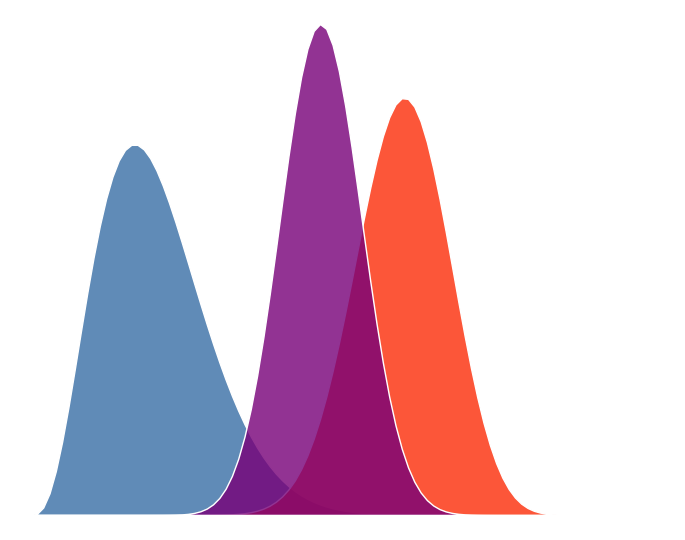
\includegraphics[width=0.8\textwidth]{figures/cover_distributions.png}

\end{center}

\newpage
\blankpage % leaves a blank page between title and TOC

\OnehalfSpacing % increasing line spacing to 1.5 (but leaving footnote to 1)

\pagenumbering{roman} % start page numbering (roman style)

{
\hypersetup{linkcolor=}
\setcounter{tocdepth}{2}
\tableofcontents
}
\hypertarget{pruxe9face}{%
\chapter*{Préface}\label{pruxe9face}}
\addcontentsline{toc}{chapter}{Préface}

\pagenumbering{arabic}

Ce document regroupe les notes de l'édition 2020 de la formation doctorale ``Introduction à la modélisation statistique bayésienne'', co-organisée par le collège des écoles doctorales de l'Université Grenoble Alpes et la Maison de la Modélisation et de la Simulation, Nanoscience, et Environnement (MaiMoSiNE).

Ces notes de cours sont organisées en suivant la structure du cours, avec un chapitre par cours, résumant les notions essentielles et donnant quelques éléments de contexte et/ou techniques supplémentaires, pour les plus curieux.

Vous pouvez télécharger la version PDF de ce document en cliquant sur l'icône PDF dans la barre d'outils figurant tout en haut de la version en ligne de ce document. Les slides, données, et codes utilisés sont également disponibles sur le répertoire Github du cours: \url{https://github.com/lnalborczyk/IMSB2020}.

Le contenu de ce livret est largement inspiré du livre \emph{Statistical rethinking} (McElreath, \protect\hyperlink{ref-mcelreath_statistical_2016}{2016}, \protect\hyperlink{ref-mcelreath_statistical_2020}{2020}) et des cours partagés librement en ligne par l'auteur. Par ailleurs, le format (HTML) du livret est en partie repris du livre \emph{Introduction to Econometrics with R} (Hanck, Arnold, Gerber, \& Schmelzer, \protect\hyperlink{ref-hanck_introduction_2018}{2018}), disponible \href{https://bookdown.org/machar1991/ITER/}{en ligne}.

Enfin, ce document est diffusé sous une licence \emph{Creative Commons Attribution - Pas d'utilisation commerciale - Partage dans les mêmes conditions} (\url{https://creativecommons.org/licenses/by-nc-sa/3.0/fr/}). Cela signifie donc que vous êtes libre de recopier / modifier / redistribuer le contenu, à condition que vous citiez la source et que vos modifications soient elle-mêmes distribuées sous la même licence (autorisant ainsi d'autres à pouvoir réutiliser à leur tour vos ajouts).

\hypertarget{introduction}{%
\chapter{Introduction à l'inférence bayésienne}\label{introduction}}

\definecolor{steelblue}{RGB}{70, 130, 180}
\definecolor{green}{RGB}{0, 153, 0}
\definecolor{purple}{RGB}{153, 0, 153}
\definecolor{orangered}{cmyk}{0, 73, 100, 0}

\epigraph{"The numbers have no way of speaking for themselves. We speak for them. We imbue them with meaning"}{Nate Silver}

Notre environnement est rempli d'incertitude. Quel temps fera-t-il demain ? Qui sera le prochain président de la République ? Vais-je apprendre quelque chose en lisant ce livret ? Tout individu est capable de se faire une idée intuitive de la réponse à ces questions (avec plus ou moins de succès) sans avoir jamais lu aucun livre traitant formellement de théorie des probabilités. Cependant, un examen plus détaillé des processus menant à ces réponses révèle une complexité et une diversité insoupçonnées. Qu'est-ce qu'une probabilité ? À quoi le concept de probabilité réfère-t-il, concrètement, dans le monde ? Et surtout, à quoi est-ce que tout cela pourrait bien nous servir dans l'analyse de données expérimentales ?

Dans ce premier chapitre, nous allons approfondir cette réflexion sur le concept de probabilité en se basant sur plusieurs définitions ayant été proposées au fil du temps. Puis, nous discuterons plus particulièrement de l'inférence bayésienne, une approche de l'inférence statistique qui utilise les probabilités comme langage pour décrire l'incertitude (et où le concept de \emph{probabilité} est à comprendre dans son acception \emph{épistémique}). Nous proposerons également un bref rappel de théorie des probabilités, une définition des probabilités conjointes, marginales, et conditionnelles, avant de dériver le théorème de Bayes à partir des règles élementaires du calcul probabiliste. Le théorème de Bayes est le ``moteur'' de l'inférence statistique bayésienne. Nous illustrerons ce mécanisme par plusieurs exemples concrets d'application.

\hypertarget{quest-ce-quune-probabilituxe9}{%
\section{Qu'est-ce qu'une probabilité ?}\label{quest-ce-quune-probabilituxe9}}

\hypertarget{axiomes-des-probabilituxe9s}{%
\subsection{Axiomes des probabilités}\label{axiomes-des-probabilituxe9s}}

Pour parler de la probabilité de certains \emph{événements} (e.g., obtenir un chiffre pair lors d'un lancer de dé), on assigne des \emph{probabilités} à ces événements. Cette assignation se fait via des \emph{fonctions de probabilité} (dont nous parlerons un peu plus tard). Tout d'abord, on définit une probabilité comme une valeur numérique assignée à un \emph{événement} \(A\), compris comme une possibilité appartenant à l'univers \(\Omega\) (l'ensemble de tous les événements possibles). Les probabilités telles que définies et utilisées dans ce cours se conforment aux axiomes suivants (Kolmogorov, \protect\hyperlink{ref-kolmogorov_foundations_1933}{1933})\footnote{On notera au passage que les axiomes de Kolmogorov représentent un exemple d'ensemble de règles permettant de définir ce qu'est une probabilité, mais que ce n'est pas le seul cadre (bien que ce soit le plus communément utilisé). Par exemple, les \href{https://en.wikipedia.org/wiki/Cox\%27s_theorem}{axiomes de Cox} offrent un cadre alternatif.} :

\begin{itemize}
\item
  \textbf{Axiome n°1} : \(\Pr(A) \geq 0\). La probabilité d'un événement \(A\) ne peut pas être négative.
\item
  \textbf{Axiome n°2} : \(\Pr(\Omega) = 1\). La somme de la probabilité de tous les événements possibles est égale à \(1\) (et donc chaque probabilité individuelle ne peut dépassr \(1\)).
\item
  \textbf{Axiome n°3} : \(\Pr(A_{1} \cup A_{2}) = \Pr(A_{1}) + \Pr(A_{2})\). La probabilité d'obtenir \emph{soit} l'événement \(A_{1}\), \emph{soit} l'événement \(A_{2}\) (sachant que ces événements sont \emph{incompatibles}) est égale à la somme de ces deux événements.
\end{itemize}

Le dernier axiome est également connu comme la \textbf{règle de la somme} et n'est valide dans cette forme que pour des événements deux à deux \emph{incompatibles} ou \emph{mutuellement exclusifs}.\footnote{Deux événements \(A_{1}\) et \(A_{2}\) sont dits \emph{incompatibles} si l'on ne peut avoir les deux en même temps, c'est à dire si \(\Pr(A_{1} \cap A_{2}) = 0\).} Il se généralise à des événements non mutuellement exclusifs de la manière suivante : \(\Pr(A_{1} \cup A_{2}) = \Pr(A_{1}) + \Pr(A_{2}) - \Pr(A_{1} \cap A_{2})\). Autrement dit et pour résumer, une probabilité est une valeur numérique positive, bornée entre 0 et 1, et qui respecte la règle de la somme.

\hypertarget{interpruxe9tations-probabilistes}{%
\subsection{Interprétations probabilistes}\label{interpruxe9tations-probabilistes}}

Bien que nous ayons donné ci-dessus une définition des probabilités, cela ne nous donne aucune indication sur la manière d'interpréter ce genre de valeur. Qu'est-ce qu'une probabilité ? Quelle genre de chose est une probabilité ? À quoi dans le monde fait référence une probabilité ? Cette question fait encore aujourd'hui couler beaucoup d'encre en philosophie de la connaissance. Nous discutons ci-dessous brièvement de quelques interprétations possibles du concept de probabilité.

\hypertarget{interpruxe9tation-classique-ou-thuxe9orique}{%
\subsubsection{Interprétation classique (ou théorique)}\label{interpruxe9tation-classique-ou-thuxe9orique}}

La première interprétation proposée est généralement la première définition que nous rencontrons dans notre cursus scolaire. Il s'agit également d'une interprétation précédent l'observation de données. En effet, dans ce cadre, une probabilité peut être calculée avant même d'avoir observé quelque donnée que ce soit, par simple connaissance du système étudié. Plus précisément, on définit la probabilité comme le rapport entre le nombre de cas favorable sur le nombre de possibles. Par exemple, si on s'intéresse à la probabilité de l'événement ``Obtenir un chiffre pair'' lors du lancer d'un dé (non pipé), alors cette probabilité peut se calculer de la manière suivante :

\[
\Pr(\text{pair}) = \frac{\text{nombre de cas favorables}}{\text{nombre de cas possibles}} = \frac{3}{6} = \frac{1}{2} \cdot
\]

Cette définition fonctionne bien pour les situations dans lesquelles il n'y a qu'un nombre \textbf{fini} de résultats possibles \textbf{équiprobables} (i.e., de même probabilité). Cependant, si on applique cette définition telle quelle à des situations plus complexes, on se rend compte que sa portée est limitée. Par exemple, si on applique cette définition à la question suivante : ``Quelle est la probabilité qu'il pleuve demain ?'', on se retrouve avec le calcul suivant.

\[\Pr(\text{pluie}) = \frac{\text{pluie}}{ \{\text{pluie, non-pluie} \} } = \frac{1}{2}\]

Et on se rend compte assez facilement que cette définition ne s'applique pas à des situations de prédiction météorologique, où il peut exister un grand nombre d'évenements possibles n'ayant pas nécessairement la même probabilité.

\hypertarget{interpruxe9tation-fruxe9quentiste-ou-empirique}{%
\subsubsection{Interprétation fréquentiste (ou empirique)}\label{interpruxe9tation-fruxe9quentiste-ou-empirique}}

L'interprétation fréquentiste du concept de probabilité propose que la probabilité est ce vers quoi tend le rapport présenté dans la section précédente lorsque le nombre d'essais tend vers l'infini (i.e., lorsque le nombre d'essais devient très important). Autement dit, la probabilité est définie de la manière suivante :

\[\Pr(x) = \lim_{n_{t} \to \infty}\frac{n_{x}}{n_{t}}\]

où \(n_{x}\) est le nombre d'occurrences de l'événement \(x\) et \(n_{t}\) le nombre total d'essais. L'interprétation \textbf{fréquentiste} postule que, à long-terme (i.e., quand le nombre d'essais s'approche de l'infini), la fréquence relative va converger \emph{exactement} vers ce qu'on appelle ``probabilité''.

\begin{Shaded}
\begin{Highlighting}[]
\KeywordTok{library}\NormalTok{(tidyverse)}

\KeywordTok{sample}\NormalTok{(}\KeywordTok{c}\NormalTok{(}\DecValTok{0}\NormalTok{, }\DecValTok{1}\NormalTok{), }\DecValTok{500}\NormalTok{, }\DataTypeTok{replace =} \OtherTok{TRUE}\NormalTok{) }\OperatorTok{\%\textgreater{}\%}
\StringTok{        }\NormalTok{data.frame }\OperatorTok{\%\textgreater{}\%}
\StringTok{        }\KeywordTok{mutate}\NormalTok{(}\DataTypeTok{x =} \KeywordTok{seq\_along}\NormalTok{(.), }\DataTypeTok{y =} \KeywordTok{cumsum}\NormalTok{(.) }\OperatorTok{/}\StringTok{ }\KeywordTok{seq\_along}\NormalTok{(.) ) }\OperatorTok{\%\textgreater{}\%}
\StringTok{        }\KeywordTok{ggplot}\NormalTok{(}\KeywordTok{aes}\NormalTok{(}\DataTypeTok{x =}\NormalTok{ x, }\DataTypeTok{y =}\NormalTok{ y), }\DataTypeTok{log =} \StringTok{"y"}\NormalTok{) }\OperatorTok{+}
\StringTok{        }\KeywordTok{geom\_line}\NormalTok{(}\DataTypeTok{lwd =} \DecValTok{1}\NormalTok{) }\OperatorTok{+}
\StringTok{        }\KeywordTok{geom\_hline}\NormalTok{(}\DataTypeTok{yintercept =} \FloatTok{0.5}\NormalTok{, }\DataTypeTok{lty =} \DecValTok{3}\NormalTok{) }\OperatorTok{+}
\StringTok{        }\KeywordTok{xlab}\NormalTok{(}\StringTok{"Nombre de lancers"}\NormalTok{) }\OperatorTok{+}
\StringTok{        }\KeywordTok{ylab}\NormalTok{(}\StringTok{"Proportion de faces"}\NormalTok{) }\OperatorTok{+}
\StringTok{        }\KeywordTok{ylim}\NormalTok{(}\DecValTok{0}\NormalTok{, }\DecValTok{1}\NormalTok{) }\OperatorTok{+}
\StringTok{        }\KeywordTok{theme\_bw}\NormalTok{(}\DataTypeTok{base\_size =} \DecValTok{12}\NormalTok{)}
\end{Highlighting}
\end{Shaded}

\begin{figure}[!htb]

{\centering 
\includegraphics[width=0.75\linewidth]{IMSB_files/figure-latex/frequency-1} 

}

\caption{Illustration de l'interprétation fréquentiste du concept de probabilité. Lorsque le nombre d'essais augmente (en abscisse), la fréquence relative (en ordonnée) converge vers la probabilité d'obtenir Face.}\label{fig:frequency}
\end{figure}

La Figure \ref{fig:frequency} illustre la \textbf{conception fréquentiste} du concept de probabilité en montrant que la probabilité est ce vers quoi la fréquence relative converge quand le nombre d'essais augmente. Une conséquence importante de cette définition est que le concept de probabilité s'applique uniquement aux \textbf{collectifs}, et non aux événements singuliers. La probabilité est définie comme la limite d'une fréquence relative, et ne permet pas de parler de la probabilité d'un événement unique.

L'interprétation fréquentiste rencontre d'autres problèmes, comme celui de la classe de référence. Considérons par exemple la question suivante : ``Quelle est la probabilité que je vive jusqu'à 80 ans ?'' Pour répondre à cette question, nous avons besoin de définir la classe de référence à partir de laquelle l'individu examiné (``je'') provient. Autrement dit, je peux estimer la probabilité qu'un individu ayant mes caractéristiques vive jusqu'à 80 ans, mais il faut d'abord déterminer quelles sont les caractéristiques importantes au regard de la question posée. Selon mon sexe biologique, ma nationalité, ou mon statut socio-économique, la réponse à cette question peut varier drastiquement. L'interprétation fréquentiste ne propose pas de procédure stricte permettant de définir la classe de référence pertinente.

Par ailleurs, cette définition ne s'aplique pas directement aux évenements qui ne peuvent pas se répéter. Par exemple, quelle est la probabilité que j'apprenne quelque chose pendant cette formation ? La réponse à cette question ne peut s'établir qu'en considérant des facteurs extérieurs à la question (e.g., le niveau de connaissance a priori), et ne peut pas reposer sur une évaluation sur le long-terme de la fréquence d'occurrence de l'événement ``apprendre quelque chose'' (cela n'aurait pas de sens de refaire la formation 1000 fois pour calculer le nombre de fois où on aura appris quelque chose).

Une autre limite importante de l'interprétation fréquentiste est la question de la résolution (ou précision) du calcul de cette probabilité. À partir de combien de lancers (d'une pièce par exemple) a-t-on une bonne approximation de la probabilité ? On sait qu'une classe finie d'événements de taille \(n\) ne peut produire que des fréquences relatives de précision \(1/n\). Jusque quand devrions-nous donc continuer ``d'échantillonner le long-terme'' avant d'avoir une estimation précise de la probabilité ?

\hypertarget{interpruxe9tation-propensionniste}{%
\subsubsection{Interprétation propensionniste}\label{interpruxe9tation-propensionniste}}

Selon l'interprétation propensionniste du concept de probabilité, les propriétés fréquentistes (i.e., à long terme) des objets (e.g., une pièce) seraient provoquées par des \emph{propriétés physiques intrinsèques} aux objets. Par exemple, une pièce biaisée va engendrer une fréquence relative (et donc une probabilité, selon l'interprétation fréquentiste) biaisée en raison de ses propriétés physiques. Pour les propensionnistes, les probabilités représentent ces caractéristiques intrinsèques, ces \textbf{propensions} à générer certaines fréquences relatives, et non les fréquences relatives en elles-mêmes.

Une conséquence intéressante de cette définition (et un progrès par rapport à l'interprétation fréquentiste) est que ces propriétés sont les propriétés d'événements individuels\ldots{} et non de séquences ! L'interprétation propensionniste nous permet donc de parler de la probabilité d'événements uniques.

\hypertarget{interpruxe9tation-logique}{%
\subsubsection{Interprétation logique}\label{interpruxe9tation-logique}}

L'interprétation logique du concept de probabilité, comme l'interprétation classique, postule que les probabilités peuvent être déterminées a priori en examinant les caractéristiques du système étudié (e.g., les caractéristiques de l'objet, l'ensemble des événements possibles, etc). Cependant, contrairement à l'interprétation classique, l'interprétation logique permet de rendre compte des événements non équiprobables. Cette interprétation se propose de réalisaer cet objectif en généralisant la logique binaire (vrai / faux) au monde probabiliste, en étudiant le degré de suppot logique fourni par un ensemble de preuves pour une hypothèse donnée. Considérons par exemple l'argument logique ci-dessous.

\textbf{Prémisse n°1} : Considérons une salle dans laquelle sont présents 10 étudiants

\textbf{Prémisse n°2} : Neuf étudiants portent un t-shirt vert

\textbf{Prémisse n°3} : Un étudiant porte un t-shirt rouge

\textbf{Prémisse n°4} : Une personne est tirée au sort\ldots{}

\par

\noindent

\rule{\textwidth}{1pt}

\textbf{Conclusion n°1} : L'étudiant tiré au sort porte un t-shirt

Cette conclusion est \emph{vraie} et l'argument qui y est attachée est \emph{valide}. Pour rappel, on dit qu'un argument est \emph{valide} lorsqu'il n'existe aucune situation logiquement possible dans laquelle tous les prémisses de l'argument soient vrais et sa conclusion fausse (Talbot, \protect\hyperlink{ref-talbot_critical_2015}{2015}). Autrement dit, si on considère les prémisses 1 à 4 comme vrais, alors il est (logiquement) impossible pour cette conclusion d'être fausse.

\par

\noindent

\rule{\textwidth}{1pt}

\textbf{Conclusion n°2} : L'étudiant tiré au sort porte un t-shirt rouge

Cette conclusion est \emph{fausse} (au sens où elle ne découle pas logiquement des prémisses) et l'argument qui y est attachée est \emph{invalide.}

\par

\noindent

\rule{\textwidth}{1pt}

\textbf{Conclusion n°3} : L'étudiant tiré au sort porte un t-shirt vert

Cette conclusion est également \emph{fausse} et l'argument qui y est attaché est \emph{invalide}. Cependant, on pourrait dire intuitivement que cette conclusion est ``un peu moins fausse'' que la conclusion précédente (je m'excuse en avance pour les logiciens qui me lisent), dans le sens où elle est ``plus fortement'' impliquée par les prémisses 1 à 4 que la conclusion n°2.

Bien que les règles de la logique formelle n'autorisent pas des conclusions à être ``plus ou moins vraies'', l'interprétation logique du concept de probabilité cherche justement à étendre les règles de la logique aux événements continus, et se propose d'utiliser le langage des probabilités dans ce but. Autrement dit, la probabilité représente donc le \emph{degré de support logique} qu'une conclusion peut avoir, relativement à un ensemble de prémices (Carnap, \protect\hyperlink{ref-carnap_logical_1950}{1950}; Keynes, \protect\hyperlink{ref-keynes_treatise_1921}{1921}).

Une conséquence intéressante de cette interprétation est que toute probabilité est \textbf{conditionnelle}, que ce soit à de l'information a priori ou, par exemple, à un ensemble de prémisses.

\hypertarget{interpruxe9tation-bayuxe9sienne}{%
\subsubsection{Interprétation bayésienne}\label{interpruxe9tation-bayuxe9sienne}}

Selon l'interprétation bayésienne (subjective), la probabilité est \textbf{une mesure du degré de croyance} (ou \emph{crédence}) ou d'\emph{incertitude}. Un événement \emph{certain} aura donc une probabilité de 1 et un événement \emph{impossible} aura une probabilité de 0.

\begin{quote}
So to assign equal probabilities to two events is not in any way an assertion that they must occur equally often in any ``random experiment''; as Jeffrey emphasized, it is only a formal way of saying ``I don't know'' (Jaynes, \protect\hyperlink{ref-jaynes_bayesian_1986}{1986}).
\end{quote}

Pour parler de probabilités, dans ce cadre, nous n'avons donc plus besoin de nous référer à la limite d'occurrence d'un événement (à sa fréquence). La probabilité est un concept abstrait faisant référence à un état de connaissanc et / ou permettant de quantifier l'incertitude liée à cet état de connaissance.

\hypertarget{interpruxe9tations-probabilistes---ruxe9sumuxe9}{%
\subsubsection{Interprétations probabilistes - résumé}\label{interpruxe9tations-probabilistes---ruxe9sumuxe9}}

Pour résumer, les différentes interprétations discutées ci-dessus peuvent être classées dans deux grandes catégories :

\begin{quote}
\textbf{Interprétation épistémique} : toute probabilité est conditionnelle à de l'information disponible (e.g., prémisses ou données). La probabilité est utilisée comme moyen de quantifier l'incertitude.

Interprétation logique (e.g., Keynes, Carnap), interprétation bayésienne (e.g., Jeffreys, de Finetti, Savage).
\end{quote}

\begin{quote}
\textbf{Interprétation physique} : les probabilités dépendent d'un état du monde, de caractéristiques physiques, elles sont indépendantes de l'information disponible (ou de l'incertitude).

Interprétation classique (e.g., Laplace, Bernouilli, Leibniz), interprétation fréquentiste (e.g., Venn, Reichenbach, von Mises).
\end{quote}

Les plus curieux d'entre vous seront ravis de trouver plus d'informations dans cet excellent article de la \emph{Stanford Encyclopedia of Philosophy} (Hájek, \protect\hyperlink{ref-sep-probability-interpret}{2019}) sur les différentes interprétations du concept de probabilité.

\hypertarget{apartuxe9---vous-avez-dit-hasard}{%
\subsection{Aparté - Vous avez dit ``hasard'' ?}\label{apartuxe9---vous-avez-dit-hasard}}

Je vous propose dans la section suivante une petite réflexion sur le concept de hasard. Considérons une suite de nombres générés ``au hasard''.

\begin{verbatim}
## [1] 79 27 98 28 42
\end{verbatim}

Qu'est-ce qui, dans la structure de cette série vous fait dire qu'elle a été générée ``au hasard'' ? Est-ce leur apparente imprédictibilité ?

Ces nombres ont été générés en utilisant la fonction \texttt{runif()}, qui comme son nom l'indique, permet de générer des nombre à partir d'une distribution Uniforme. Cette fonction (comme d'autres telles que \texttt{rnorm()} ou \texttt{rbinom()}) utilisent des générateurs de nombre aléatoire, permettant de générer des séries de nombres qui ``ressemblent'' à des séries générées au hasard. On peut savoir quel est générateur est utilisé en \texttt{R} via la commande suivante.

\begin{Shaded}
\begin{Highlighting}[]
\KeywordTok{RNGkind}\NormalTok{()[}\DecValTok{1}\NormalTok{] }\CommentTok{\# retourne le RNG par défaut}
\end{Highlighting}
\end{Shaded}

\begin{verbatim}
## [1] "Mersenne-Twister"
\end{verbatim}

Inventé par Makoto Matsumoto et Takuji Nishimura en 1997, le \href{https://en.wikipedia.org/wiki/Mersenne_Twister}{Mersenne Twister} est un générateur de nombres pseudo-aléatoires. L'algorithme Mersenne-Twister est (\emph{était}) le générateur par défaut en \texttt{R}, \texttt{Python}, \texttt{Ruby}, ou encore \texttt{Matlab}. Son fonctionnement est illustré dans la Figure \ref{fig:mersenne}.

\begin{figure}[!htb]

{\centering 
\includegraphics[width=1\linewidth]{figures/mersenne} 

}

\caption{Illustration de l'algorithme Mersenne-Twister algorithm. Figure from Wikipedia.}\label{fig:mersenne}
\end{figure}

Cet algorithme est relativement complexe, mais pour simplifier, disons que la tâche principale réalisée par l'algorithme est de transformer un \emph{input} (en l'ocurrence, une ``graine'') en un \emph{output} (la série de nombres). L'idée générale étant de donner en sortie une suite de nombres ayant le moins de rapport possible avec l'entrée. Notons néanmoins que la notion de ``moins de rapport possible'' est ambigue. En effet, cette notion dépend du degré de naiveté de l'agent qui observe le fonctionnement de l'algorithme. Si l'agent ignore tout du fonctionnement de l'algorithme, alors en effet la série de nombres obtenu en sortie de l'algorithme semblera ``sans rapport'' avec la graine (i.e., la valeur de départ de l'algorithme). Au contraire, si l'agent connait le fonctionnement de l'algorithme, alors la série de nombres obtenue en sortie de l'algorithme est parfaitement prédictible (si on admet qu'on dispose de la puissance de calcul nécessaire pour reproduire les étapes de l'algorithme) sachant la graine de départ.

Afin d'illustrer plus en détails cette idée, considérons à nouveau la série de cinq nombres générés au début de cette section. Les nombres générés ci-dessus ont été générés de la manière suivante :

\[Y_{i} \sim \mathrm{Uniform}(10, 100) \cdot\]
Autrement dit, on a ``tiré'' cinq nombres issus d'une distribution uniforme borne entre 10 et 100.

\begin{Shaded}
\begin{Highlighting}[]
\CommentTok{\# on fixe la graine afin de pouvoir reproduire les résultats}
\KeywordTok{set.seed}\NormalTok{(}\DecValTok{666}\NormalTok{)}

\CommentTok{\# on tire cinq entiers issus de Uniform(10, 100)}
\KeywordTok{as.integer}\NormalTok{(}\KeywordTok{runif}\NormalTok{(}\DecValTok{5}\NormalTok{, }\DecValTok{10}\NormalTok{, }\DecValTok{100}\NormalTok{) )}
\end{Highlighting}
\end{Shaded}

\begin{verbatim}
## [1] 79 27 98 28 42
\end{verbatim}

\begin{Shaded}
\begin{Highlighting}[]
\CommentTok{\# on tire six entiers issus de Uniform(10, 100)}
\KeywordTok{set.seed}\NormalTok{(}\DecValTok{666}\NormalTok{)}
\KeywordTok{as.integer}\NormalTok{(}\KeywordTok{runif}\NormalTok{(}\DecValTok{6}\NormalTok{, }\DecValTok{10}\NormalTok{, }\DecValTok{100}\NormalTok{) )}
\end{Highlighting}
\end{Shaded}

\begin{verbatim}
## [1] 79 27 98 28 42 76
\end{verbatim}

Pour résumer, si je connais la \emph{graine} d'origine (i.e., le ``départ'' de l'algorithme) et le fonctionnement précis de l'algorithme, je peux prédire les nombres qui vont être générés. Il sera alors difficile de soutenir que ces nombres auront été générés ``au hasard''\ldots{}

Selon \href{https://fr.wikipedia.org/wiki/Hasard}{Wikipédia}, ``Le hasard est un concept indiquant l'aspect aléatoire des choses, des événements ou encore des décisions, signalant ainsi l'impossibilité de prévoir avec certitude un fait quelconque. Ainsi, pour éclairer le sens du mot, il peut-être dit que le hasard est synonyme d'« imprévisibilité », ou « imprédictibilité »''. D'autres définitions sont proposées ci-dessous :

\begin{quote}
\emph{Ce que nous appelons hasard n'est et ne peut être que la cause ignorée d'un effet connu.} -- Voltaire
\end{quote}

\begin{quote}
\emph{Le hasard, ce sont les lois que nous ne connaissons pas.} -- Émile Borel
\end{quote}

\begin{quote}
\emph{Randomness is a proxy for lack of knowledge.} -- Richard McElreath
\end{quote}

Le hasard apparaît donc comme un \textbf{état subjectif d'indétermination des causes}. Pour parler de l'incertain (i.e., pour quantifier l'incertitude), on utilise les probabilités comme langage.

\hypertarget{un-peu-de-logique}{%
\section{Un peu de logique}\label{un-peu-de-logique}}

Le but de cette section est de proposer une courte (et très incomplète) introduction à la logique, afin de pouvoir analyser dans une section suivante l'argument central de l'inférence fréquentiste, et d'illustrer les similarités entre la logique binaire et le fonctionnement de l'inférence bayésienne. Nous allons tout d'abord commencer par définir les termes utilisés (cf.~Talbot, \protect\hyperlink{ref-talbot_critical_2015}{2015}).

\BeginKnitrBlock{definition}[Argument]
\protect\hypertarget{def:argument}{}{\label{def:argument} \iffalse (Argument) \fi{} }Un \emph{argument} est un ensemble de propositions dans lequel une propositions est affirmée sur la base d'autres propositions.
\EndKnitrBlock{definition}

Un argument (du moins tel que défini ici) est donc composé de différentes propositions. Parmi ces propositions, certaines vont être utilisées pour \emph{affirmer} une autre proposition.

\BeginKnitrBlock{definition}[Conclusion]
\protect\hypertarget{def:concusion}{}{\label{def:concusion} \iffalse (Conclusion) \fi{} }La \emph{conclusion} est l'affirmation faite sur la base d'autres propositions.
\EndKnitrBlock{definition}

\BeginKnitrBlock{definition}[Prémisses]
\protect\hypertarget{def:pruxe9misse}{}{\label{def:prémisse} \iffalse (Prémisses) \fi{} }Les \emph{prémisses} d'un argument sont les raisons offertes qui permettent d'affirmer la conclusion.
\EndKnitrBlock{definition}

Pour résumer, un \emph{argument} est un ensemble de propositions, parmis lesquelles des \emph{prémisses} sont utilisées pour affirmer une \emph{conclusion}. Les propositions qui composent un \emph{argument} (i.e., les prémisses et la conclusion) peuvent être \emph{vraies} ou \emph{fausses} mais l'argument ne peut pas être \emph{vrai} ou \emph{faux}. Un argument est seulement \emph{valide} ou \emph{invalide}.

\BeginKnitrBlock{definition}[Validité]
\protect\hypertarget{def:valide}{}{\label{def:valide} \iffalse (Validité) \fi{} }Un argument est dit \emph{valide} si et seulement si il n'existe aucune situation logiquement possible dans laquelle tous les prémisses de l'argument soient vrais et sa conclusion fausse.
\EndKnitrBlock{definition}

\BeginKnitrBlock{definition}[Invalidité]
\protect\hypertarget{def:invalide}{}{\label{def:invalide} \iffalse (Invalidité) \fi{} }Un argument est dit \emph{invalide} si et seulement si il existe aucune situation logiquement possible dans laquelle tous les prémisses de l'argument soient vrais et sa conclusion fausse.
\EndKnitrBlock{definition}

Pour résumer, un argument est un ensemble de \emph{propositions}, dont certaines d'entre elles (les prémisses) sont utilisées pour affirmer (ou justifier) une autre (la conclusion). Ces propositions peuvent être vraies ou fausses mais un argument peut seulement être \emph{valide} ou \emph{invalide}. Un argument est dit \emph{valide} lorsqu'il est logiquement \emph{impossible} pour la conclusion d'être fausse (sachant que les prémisses sont \emph{vraies}).

\hypertarget{quelques-syllogismes-connus}{%
\subsection{Quelques syllogismes connus}\label{quelques-syllogismes-connus}}

\begin{figure}[!htb]

{\centering 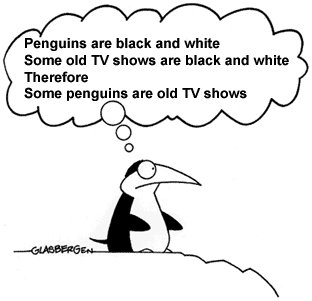
\includegraphics[width=0.5\linewidth]{figures/penguin} 

}

\caption{Un pingouin s'essayant à la logique. Source : https://www.pinterest.com/pin/465418942711158498/.}\label{fig:penguin}
\end{figure}

Un syllogisme est un raisonnement logique qui met en relation \emph{au moins} trois propositions : au moins deux prémisses et une conclusion. Afin d'illustrer les définitions proposées ci-dessus, nous allons maintenant examiner quelques exemples. Savez-vous reconnaître les arguments valides et invalides ?

\textbf{Argument n°1}

\begin{itemize}
\tightlist
\item
  Prémisse n°1 : Si un suspect ment, il transpire.
\item
  Prémisse n°2 : (On observe que) Ce suspect transpire.
\item
  Conclusion : Par conséquent, ce suspect ment.
\end{itemize}

Cet argument est \emph{invalide} car (on applique la définition \ref{def:valide}) il existe des situations dans lesquelles à la fois les prémisses 1 et 2 sont vraies, et pourtant la conclusion est fausse. Par exemple, il se peut que le suspect transpire pour d'autres raisons que le mensonge (e.g., la température de la salle d'interrogatoire).

\textbf{Argument n°2}

\begin{itemize}
\tightlist
\item
  Prémisse n°1 : Si un suspect transpire, il ment.
\item
  Prémisse n°2 : (On observe que) Ce suspect ne transpire pas.
\item
  Conclusion : Par conséquent, ce suspect ne ment pas.
\end{itemize}

Cet argument est également \emph{invalide} car il existe des situations dans lesquelles à la fois les prémisses 1 et 2 sont vraies, et pourtant la conclusion est fausse. Par exemple\ldots{}

\textbf{Argument n°3}

\begin{itemize}
\tightlist
\item
  Prémisse n°1 : Tous les menteurs transpirent.
\item
  Prémisse n°2 : (On observe que) Ce suspect ne transpire pas.
\item
  Conclusion : Par conséquent, ce suspect n'est pas un menteur.
\end{itemize}

Cet argument est \emph{valide} car il n'existe aucune situation dans laquelle à la fois les prémisses 1 et 2 sont vraies et la conclusion serait fausse. Autrement dit, si les prémisses 1 et 2 sont vraies, il est \emph{logiquement impossible} pour la conclusion d'être fausse. Nous allons maintenant examiner quelques raisonnements valides et invalides inconnus afin de nous aider à les repérer plus facilement.

\hypertarget{arguments-invalides}{%
\subsubsection{Arguments invalides}\label{arguments-invalides}}

\begin{itemize}
\item
  \emph{Affirmation du conséquent}: \(\dfrac{A \Rightarrow B, \ B}{A}\)
\item
  Si il a plu, alors le sol est mouillé (A implique B). Le sol est mouillé (B). Donc il a plu (A).
\item
  \emph{Négation de l'antécédent}: \(\dfrac{A \Rightarrow B, \ \neg A}{\neg B}\)
\item
  Si il a plu, alors le sol est mouillé (A implique B). Il n'a pas plus (non A). Donc le sol n'est pas mouillé (non B).
\end{itemize}

\hypertarget{arguments-valides}{%
\subsubsection{Arguments valides}\label{arguments-valides}}

\begin{itemize}
\item
  \emph{Modus ponens}: \(\dfrac{A \Rightarrow B, \ A}{B}\)
\item
  Si on est lundi, alors John ira au travail (A implique B). On est lundi (A). Donc John ira au travail (B).
\item
  \emph{Modus tollens}: \(\dfrac{A \Rightarrow B, \ \neg B}{\neg A}\)
\item
  Si mon chien détecte un intru, alors il aboie (A implique B). Mon chien n'a pas aboyé (non B). Donc il n'a pas détecté d'intrus (non A).
\end{itemize}

\hypertarget{logique-fruxe9quentisme-et-raisonnement-probabiliste}{%
\subsection{Logique, fréquentisme et raisonnement probabiliste}\label{logique-fruxe9quentisme-et-raisonnement-probabiliste}}

Le \emph{modus tollens} est un des raisonnements logiques les plus importants et les plus performants. Dans le cadre de l'inférence statistique, il s'applique parfaitement au cas suivant: ``Si \(H_{0}\) est vraie, alors \(x\) ne devrait pas se produire. On observe \(x\). Alors \(H_{0}\) est fausse''.

Mais nous avons le plus souvent affaire à des hypothèses ``continues'', probabilistes.

L'inférence fréquentiste (Fishérienne) est elle aussi probabiliste, de la forme ``Si \(H_{0}\) est vraie, alors \(x\) est peu probable. On observe \(x\). Alors \(H_{0}\) est peu probable.''

Or cet argument est invalide, le \emph{modus tollens} ne s'applique pas au monde probabiliste (e.g., \href{http://citeseerx.ist.psu.edu/viewdoc/download?doi=10.1.1.505.9968\&rep=rep1\&type=pdf}{Pollard \& Richardson, 1987}; \href{http://www.ejwagenmakers.com/2016/RouderEtAl2016FreeLunch.pdf}{Rouder, Morey, Verhagen, Province, \& Wagenmakers, 2016}).

Par exemple: \emph{si un individu est un homme, alors il est peu probable qu'il soit pape. François est pape. François n'est donc certainement pas un homme\ldots{}}

\hypertarget{luxe9chec-de-la-falsification}{%
\subsection{L'échec de la falsification}\label{luxe9chec-de-la-falsification}}

\emph{Poppérisme naïf}: la science progresse par falsification logique, donc la statistique devrait viser la falsification. Mais\ldots{}

\begin{itemize}
\tightlist
\item
  Les hypothèses théoriques ne sont pas les modèles (hypothèses statistiques)
\end{itemize}

\begin{quote}
\emph{Models are devices that connect theories to data. A model is an instanciation of a theory as a set of probabilistic statements} (\href{https://www.collabra.org/articles/10.1525/collabra.28/}{Rouder et al., 2016}).
\end{quote}

\begin{itemize}
\tightlist
\item
  Nos hypothèses sont souvent probabilistes
\item
  Erreurs de mesure
\item
  La falsification concerne le problème de la démarcation, pas celui de la méthode
\item
  La science est une technologie sociale, la falsification est \textbf{consensuelle}, et non pas logique
\end{itemize}

\hypertarget{lapproche-par-comparaison-de-moduxe8les}{%
\subsection{L'approche par comparaison de modèles}\label{lapproche-par-comparaison-de-moduxe8les}}

On s'intéresse au lien entre deux variables aléatoires continues, \(x\) et \(y\).

\begin{figure}[!htb]

{\centering 
\includegraphics[width=0.75\linewidth]{IMSB_files/figure-latex/modelcomp1-1} 

}

\caption{Blah blah...}\label{fig:modelcomp1}
\end{figure}

L'hypothèse de modélisation la plus simple est de postuler une relation linéaire.

\begin{figure}[!htb]

{\centering 
\includegraphics[width=0.75\linewidth]{IMSB_files/figure-latex/modelcomp2-1} 

}

\caption{Blah blah...}\label{fig:modelcomp2}
\end{figure}

Cette description peut-être \emph{améliorée} pour mieux prendre en compte les données qui s'écartent de la prédiction linéaire.

\begin{figure}[!htb]

{\centering 
\includegraphics[width=0.75\linewidth]{IMSB_files/figure-latex/modelcomp3-1} 

}

\caption{Blah blah...}\label{fig:modelcomp3}
\end{figure}

Un ensemble de \(N\) points peut être \emph{exhaustivement} (sans erreur) décrit par une fonction polynomiale d'ordre \(N-1\). Augmenter la complexité du modèle améliore donc la précision de notre description des données mais réduit la généralisabilité de ses prédictions (\emph{bias-variance tradeoff}).

\begin{figure}[!htb]

{\centering 
\includegraphics[width=0.75\linewidth]{IMSB_files/figure-latex/modelcomp4-1} 

}

\caption{Blah blah...}\label{fig:modelcomp4}
\end{figure}

Nous avons besoin d'outils qui prennent en compte le rapport \emph{qualité de la description} / \emph{complexité}, c'est à dire la \textbf{parcimonie} des modèles (e.g., AIC, WAIC)\ldots{}

Nous avons besoin d'un cadre pour développer des modèles cohérents. Nos outils:

\begin{itemize}
\tightlist
\item
  \emph{Bayesian data analysis}, utiliser les probabilités pour décrire l'incertitude
\item
  \emph{Multilevel modelling}, des modèles à multiples niveaux d'incertitude
\item
  Approche par comparaison de modèles, au lieu d'essayer de falsifier un \emph{null model}, comparer des modèles intéressants (AIC, WAIC)
\end{itemize}

\hypertarget{probluxe8me-du-sac-de-billes-mcelreath_statistical_2016}{%
\section{\texorpdfstring{Problème du sac de billes (McElreath, \protect\hyperlink{ref-mcelreath_statistical_2016}{2016})}{Problème du sac de billes (McElreath, 2016)}}\label{probluxe8me-du-sac-de-billes-mcelreath_statistical_2016}}

Imaginons que nous disposions d'un sac contenant 4 billes. Ces billes peuvent être soit blanches, soit bleues. Nous savons qu'il y a précisément 4 billes, mais nous ne connaissons pas le nombre de billes de chaque couleur.

Nous savons cependant qu'il existe cinq possibilités (que nous considérons comme nos \emph{hypothèses}) :

\[
\begin{aligned}
&\text{Hypothèse n°1 : } \LARGE \circ \circ \circ \circ \\
&\text{Hypothèse n°2 : } \LARGE \color{steelblue}{\bullet} \color{black}{\circ} \circ \circ \\
&\text{Hypothèse n°3 : } \LARGE \color{steelblue}{\bullet} \color{steelblue}{\bullet} \color{black}{\circ} \circ \\
&\text{Hypothèse n°4 : } \LARGE \color{steelblue}{\bullet} \color{steelblue}{\bullet} \color{steelblue}{\bullet} \color{black}{\circ} \\
&\text{Hypothèse n°5 : } \LARGE \color{steelblue}{\bullet} \color{steelblue}{\bullet} \color{steelblue}{\bullet} \color{steelblue}{\bullet} \\
\end{aligned}
\]

Le but est de déterminer quelle combinaison serait la plus probable, \textbf{sachant certaines observations}. Imaginons que l'on tire trois billes à la suite, avec remise, et que l'on obtienne la séquence suivante : \(\LARGE \color{steelblue}{\bullet} \color{black}{\circ} \color{steelblue}{\bullet}\).

Cette séquence représente nos données. À partir de là, quelle \textbf{inférence} peut-on faire sur le contenu du sac ? En d'autres termes, que peut-on dire de la probabilité de chaque hypothèse ?

\hypertarget{uxe9numuxe9rer-les-possibilituxe9s}{%
\subsection{Énumérer les possibilités}\label{uxe9numuxe9rer-les-possibilituxe9s}}

Une stratégie consiste à compter le nombre de possibilités menant aux données obtenues à chaque tirage\ldots{} Par exemple, si nous considérons l'hypothèse n°2 (i.e., on se place dans un cadre dans lequel cette hypothèse est ``vraie''), on peut représenter l'arbre des issues possibles. La Figure \ref{fig:garden1} représente\ldots{}

\begin{figure}[!htb]

{\centering 
\includegraphics[width=0.75\linewidth]{IMSB_files/figure-latex/garden1-1} 

}

\caption{Représentation de l'ensemble des issues possible au premier tirage selon l'hypothèse n°2.}\label{fig:garden1}
\end{figure}

Au deuxième tirage\ldots{} La Figure \ref{fig:garden2} représente\ldots{}

\begin{figure}[!htb]

{\centering 
\includegraphics[width=0.75\linewidth]{IMSB_files/figure-latex/garden2-1} 

}

\caption{Blah blah...}\label{fig:garden2}
\end{figure}

Au troisième tirage\ldots{} La Figure \ref{fig:garden3} représente\ldots{}

\begin{figure}[!htb]

{\centering 
\includegraphics[width=0.75\linewidth]{IMSB_files/figure-latex/garden3-1} 

}

\caption{Blah blah...}\label{fig:garden3}
\end{figure}

La Figure \ref{fig:garden4} représente le nombre de ``chemins'' qui mènent au résultat obtenu\ldots{} Sous cette hypothèse, \(3\) chemins (sur \(4^{3} = 64\)) conduisent au résultat obtenu. Qu'en est-il des autres hypothèses?

\begin{figure}[!htb]

{\centering 
\includegraphics[width=0.75\linewidth]{IMSB_files/figure-latex/garden4-1} 

}

\caption{Blah blah...}\label{fig:garden4}
\end{figure}

La Figure \ref{fig:garden5} représente\ldots{}

\begin{figure}[!htb]

{\centering 
\includegraphics[width=0.75\linewidth]{IMSB_files/figure-latex/garden5-1} 

}

\caption{Blah blah...}\label{fig:garden5}
\end{figure}

\hypertarget{comparer-les-hypothuxe8ses}{%
\subsection{Comparer les hypothèses}\label{comparer-les-hypothuxe8ses}}

On peut comparer les hypothèses par leur propension au mener au résultat obtenu (i.e., aux données). Plus précisément, si l'on compare le nombre de chemins possibles pour chaque hypothèse\ldots{}

\begin{table}[!htb]

\begin{center}
\begin{threeparttable}

\caption{\label{tab:hypothesis-comparison}Comparer des hypothèses en comparant le nombre de manières qu'elles ont de produire les données observées.}

\begin{tabular}{cc}
\toprule
Hypothèse & Façons d'obtenir les données\\
\midrule
$\LARGE \circ \circ \circ \circ$ & $0 \times 4 \times 0 = 0$\\
$\LARGE \color{steelblue}{\bullet} \circ \circ \circ$ & $1 \times 3 \times 1 = 3$\\
$\LARGE \color{steelblue}{\bullet} \color{steelblue}{\bullet} \circ \circ$ & $2 \times 2 \times 2 = 8$\\
$\LARGE \color{steelblue}{\bullet} \color{steelblue}{\bullet} \color{steelblue}{\bullet} \circ$ & $3 \times 1 \times 3 = 9$\\
$\LARGE \color{steelblue}{\bullet} \color{steelblue}{\bullet} \color{steelblue}{\bullet} \color{steelblue}{\bullet}$ & $4 \times 0 \times 4 = 0$\\
\bottomrule
\end{tabular}

\end{threeparttable}
\end{center}

\end{table}

Au vu des données, l'hypothèse n°4 est la plus \emph{probable} car c'est l'hypothèse qui \textbf{maximise le nombre de manières possibles d'obtenir les données obtenues}.

\hypertarget{accumulation-duxe9vidence}{%
\subsection{Accumulation d'évidence}\label{accumulation-duxe9vidence}}

Dans le cas précédent, nous avons considéré que toutes les hypothèses étaient équiprobables a priori (suivant le \href{https://en.wikipedia.org/wiki/Principle_of_indifference}{principe d'indifférence}). Cependant, on pourrait avoir de l'information a priori, provenant de nos connaissances (des particularités des sacs de billes par exemple) ou de données antérieures.

Imaginons que nous tirions une nouvelle bille du sac, comment incorporer cette nouvelle donnée ?

Il suffit d'appliquer la même stratégie que précédemment, et de mettre à jour le dernier compte en le multipliant par ces nouvelles données. \emph{Yesterday's posterior is today's prior} (Lindley, \protect\hyperlink{ref-lindley_philosophy_2001}{2001}).

\begin{table}[!htb]

\begin{center}
\begin{threeparttable}

\caption{\label{tab:accumulation}Illustration de l'accumulation d'information dans le cadre bayésien.}

\begin{tabular}{cccc}
\toprule
Hypothèse & Façons de produire $\color{steelblue}{\bullet}$ & Compte précédent & Nouveau compte\\
\midrule
$\LARGE \circ \circ \circ \circ$ & $0$ & $0$ & $0 \times 0 = 0$\\
$\LARGE \color{steelblue}{\bullet} \circ \circ \circ$ & $1$ & $3$ & $3 \times 1 = 3$\\
$\LARGE \color{steelblue}{\bullet} \color{steelblue}{\bullet} \circ \circ$ & $2$ & $8$ & $8 \times 2 = 16$\\
$\LARGE \color{steelblue}{\bullet} \color{steelblue}{\bullet} \color{steelblue}{\bullet} \circ$ & $3$ & $9$ & $9 \times 3 = 27$\\
$\LARGE \color{steelblue}{\bullet} \color{steelblue}{\bullet} \color{steelblue}{\bullet} \color{steelblue}{\bullet}$ & $4$ & $0$ & $0 \times 4 = 0$\\
\bottomrule
\end{tabular}

\end{threeparttable}
\end{center}

\end{table}

\hypertarget{incorporer-un-prior}{%
\subsection{Incorporer un prior}\label{incorporer-un-prior}}

Supposons maintenant qu'un employé de l'usine de fabrication des billes nous dise que les billes bleues sont rares\ldots{} Cet employé nous dit que pour chaque sac contenant 3 billes bleues, ils fabriquent deux sacs en contenant seulement deux, et trois sacs en contenant seulement une. Il nous apprend également que tous les sacs contiennent au moins une bille bleue et une bille blanche\ldots{}

\begin{table}[!htb]

\begin{center}
\begin{threeparttable}

\caption{\label{tab:prior-table}Illustration de l'intégration d'information a priori dans le cadre bayésien.}

\begin{tabular}{cccc}
\toprule
Hypothèse & Compte précédent & Prior usine & Nouveau compte\\
\midrule
$\LARGE \circ \circ \circ \circ$ & $0$ & $0$ & $0 \times 0 = 0$\\
$\LARGE \color{steelblue}{\bullet} \circ \circ \circ$ & $3$ & $3$ & $3 \times 3 = 9$\\
$\LARGE \color{steelblue}{\bullet} \color{steelblue}{\bullet} \circ \circ$ & $16$ & $2$ & $16 \times 2 = 32$\\
$\LARGE \color{steelblue}{\bullet} \color{steelblue}{\bullet} \color{steelblue}{\bullet} \circ$ & $27$ & $1$ & $27 \times 1 = 27$\\
$\LARGE \color{steelblue}{\bullet} \color{steelblue}{\bullet} \color{steelblue}{\bullet} \color{steelblue}{\bullet}$ & $0$ & $0$ & $0 \times 4 = 0$\\
\bottomrule
\end{tabular}

\end{threeparttable}
\end{center}

\end{table}

\hypertarget{des-uxe9numuxe9rations-aux-probabilituxe9s}{%
\subsection{Des énumérations aux probabilités}\label{des-uxe9numuxe9rations-aux-probabilituxe9s}}

La plausibilité d'une hypothèse après avoir observé certaines données est proportionnelle au nombre de façons qu'a cette hypothèse de produire les données observées, multiplié par sa plausibilité a priori.

\begin{equation}
p(hypothesis|data)\propto p(data|hypothesis) \times p(hypothesis)
\label{eq:plausib}
\end{equation}

Voir équation \eqref{eq:plausib}\ldots{} Pour passer des \emph{plausibilités} aux \emph{probabilités}, il suffit de standardiser ces plausibilités pour que la somme des plausibilités de toutes les hypothèses possibles soit égale à \(1\).

\[p(hypothesis|data) = \frac{p(data|hypothesis) \times p(hypothesis)}{sum\ of\ products}\]

Définissons \(p\) comme la proportion de billes bleues.

\begin{table}[!htb]

\begin{center}
\begin{threeparttable}

\caption{\label{tab:enumeration-table}Calcul de la probabilité d'une hypothèse.}

\begin{tabular}{cccc}
\toprule
Hypothèse & $p$ & Manières de produire les données & Probabilité\\
\midrule
$\LARGE \circ \circ \circ \circ$ & $0$ & $0$ & $0$\\
$\LARGE \color{steelblue}{\bullet} \circ \circ \circ$ & $0.25$ & $3$ & $0.15$\\
$\LARGE \color{steelblue}{\bullet} \color{steelblue}{\bullet} \circ \circ$ & $0.5$ & $8$ & $0.40$\\
$\LARGE \color{steelblue}{\bullet} \color{steelblue}{\bullet} \color{steelblue}{\bullet} \circ$ & $0.75$ & $9$ & $0.45$\\
$\LARGE \color{steelblue}{\bullet} \color{steelblue}{\bullet} \color{steelblue}{\bullet} \color{steelblue}{\bullet}$ & $1$ & $0$ & $0$\\
\bottomrule
\end{tabular}

\end{threeparttable}
\end{center}

\end{table}

\begin{Shaded}
\begin{Highlighting}[]
\NormalTok{ways \textless{}{-}}\StringTok{ }\KeywordTok{c}\NormalTok{(}\DecValTok{0}\NormalTok{, }\DecValTok{3}\NormalTok{, }\DecValTok{8}\NormalTok{, }\DecValTok{9}\NormalTok{, }\DecValTok{0}\NormalTok{)}
\NormalTok{ways }\OperatorTok{/}\StringTok{ }\KeywordTok{sum}\NormalTok{(ways)}
\end{Highlighting}
\end{Shaded}

\begin{verbatim}
## [1] 0.00 0.15 0.40 0.45 0.00
\end{verbatim}

\hypertarget{notations-terminologie}{%
\subsection{Notations, terminologie}\label{notations-terminologie}}

\begin{itemize}
\tightlist
\item
  \(\theta\) un paramètre ou vecteur de paramètres (e.g., la proportion de billes bleues)
\item
  \(\color{orangered}{p(x\vert \theta)}\) { la probabilité conditionnelle des données \(x\) sachant le paramètre \(\theta\) } \(\color{orangered}{[p(x | \theta = \theta)]}\)
\item
  \(\color{orangered}{p(x\vert \theta)}\) { une fois que la valeur de \(x\) est connue, est vue comme la fonction de vraisemblance (\emph{likelihood}) du paramètre \(\theta\). Attention, il ne s'agit pas d'une distribution de probabilité (n'intègre pas à 1). } \(\color{orangered}{[p(x = x | \theta)]}\)
\item
  \(\color{steelblue}{p(\theta)}\) { la probabilité a priori de \(\theta\)}
\item
  \(\color{purple}{p(\theta \vert x)}\) { la probabilité a posteriori de \(\theta\) (sachant \(x\))}
\item
  \(\color{green}{p(x)}\) { la probabilité marginale de \(x\) (sur \(\theta\))}
\end{itemize}

\[
\color{purple}{p(\theta \vert x)} = \dfrac{\color{orangered}{p(x\vert \theta)} \color{steelblue}{p(\theta)}}{\color{green}{p(x)}} = \dfrac{\color{orangered}{p(x\vert \theta)} \color{steelblue}{p(\theta)}}{\color{green}{\sum\limits_{\theta}p(x|\theta)p(\theta)}} = \dfrac{\color{orangered}{p(x\vert \theta)} \color{steelblue}{p(\theta)}}{\color{green}{\int\limits_{\theta}p(x|\theta)p(\theta)\mathrm{d}x}} \propto \color{orangered}{p(x\vert \theta)} \color{steelblue}{p(\theta)}
\]

Dans ce cadre, pour chaque problème, nous allons suivre 3 étapes:

\begin{itemize}
\tightlist
\item
  Construire le modèle (l'histoire des données): \emph{likelihood} + \emph{prior}
\item
  Mettre à jour grâce aux données (\emph{updating}), calculer la probabilité \emph{a posteriori}
\item
  Evaluer le modèle, \emph{fit}, sensibilité, résumer les résultats, ré-ajuster
\end{itemize}

\begin{quote}
\emph{Bayesian inference is really just counting and comparing of possibilities {[}\ldots{]} in order to make good inference about what actually happened, it helps to consider everything that could have happened} (McElreath, 2015).
\end{quote}

\hypertarget{rappels-de-probabilituxe9}{%
\section{Rappels de probabilité}\label{rappels-de-probabilituxe9}}

\hypertarget{loi-de-probabilituxe9-cas-discret}{%
\subsection{Loi de probabilité, cas discret}\label{loi-de-probabilituxe9-cas-discret}}

\BeginKnitrBlock{definition}[Fonction de masse de probabilité]
\protect\hypertarget{def:PMF}{}{\label{def:PMF} \iffalse (Fonction de masse de probabilité) \fi{} }La fonction de masse de probabilité \(p\) d'une variable aléatoire \(X\) is la fonction \(p : \mathbb{R} \rightarrow [0, 1]\), définie par :

\[p(a) = \Pr(X = a) \quad \text{for} - \infty < a < \infty\]
\EndKnitrBlock{definition}

Une fonction de masse (\emph{probability mass function}, ou \emph{PMF}) est une fonction qui attribue une probabilité à chaque valeur d'une variable aléatoire. Exemple de la distribution binomiale pour une pièce non biaisée (\(\theta = 0.5\)), probabilité d'obtenir \(N\) faces sur 10 lancers.

\begin{figure}[!htb]

{\centering 
\includegraphics[width=0.5\linewidth]{IMSB_files/figure-latex/binomial-barplot-1} 

}

\caption{Blah blah...}\label{fig:binomial-barplot}
\end{figure}

\begin{Shaded}
\begin{Highlighting}[]
\CommentTok{\# PMFs sum to 1}
\KeywordTok{dbinom}\NormalTok{(}\DataTypeTok{x =} \DecValTok{0}\OperatorTok{:}\DecValTok{10}\NormalTok{, }\DataTypeTok{size =} \DecValTok{10}\NormalTok{, }\DataTypeTok{prob =} \FloatTok{0.5}\NormalTok{) }\OperatorTok{\%\textgreater{}\%}\StringTok{ }\NormalTok{sum}
\end{Highlighting}
\end{Shaded}

\begin{verbatim}
## [1] 1
\end{verbatim}

\hypertarget{loi-de-probabilituxe9-cas-continu}{%
\subsection{Loi de probabilité, cas continu}\label{loi-de-probabilituxe9-cas-continu}}

\BeginKnitrBlock{definition}[Fonction de densité de probabilité]
\protect\hypertarget{def:PDF}{}{\label{def:PDF} \iffalse (Fonction de densité de probabilité) \fi{} }Une variable aléatoire \(X\) est dite \emph{continue} si pour une fonction donnée \(p : \mathbb{R} \rightarrow \mathbb{R}\) et pour tout nombres \(a\) et \(b\) avec \(a \leq b\),

\[\Pr(a \leq X \leq b) = \int_{a}^{b} p(x) \mathrm{d} x\]

La fonction \(p\) doit satisfaire la condition \(p(x) \geq 0\) pour tout \(x\) et \(\int_{-\infty}^{\infty} p(x) \mathrm{d} x = 1\). On appelle \(p\) la fonction de densité de probabilité (ou densité de probabilité) de \(X\).
\EndKnitrBlock{definition}

Une fonction de densité de probabilité (\emph{probability density function}, ou \emph{PDF}), est une fonction qui permet de représenter une loi de probabilité sous forme d'intégrales (l'équivalent de la PMF pour des variables aléatoires strictement continues).

\begin{figure}[!htb]

{\centering 
\includegraphics[width=0.5\linewidth]{IMSB_files/figure-latex/pdf-plot-1} 

}

\caption{Blah blah...}\label{fig:pdf-plot}
\end{figure}

\begin{Shaded}
\begin{Highlighting}[]
\CommentTok{\# PDFs integrate to 1}
\KeywordTok{integrate}\NormalTok{(dnorm, }\OperatorTok{{-}}\OtherTok{Inf}\NormalTok{, }\OtherTok{Inf}\NormalTok{, }\DataTypeTok{mean =} \DecValTok{100}\NormalTok{, }\DataTypeTok{sd =} \DecValTok{15}\NormalTok{)}
\end{Highlighting}
\end{Shaded}

\begin{verbatim}
## 1 with absolute error < 1.3e-06
\end{verbatim}

\ldots{}

\begin{keyconcepts}[Variable aléatoire continue]{1.1}
Une variable aléatoire continue peut prendre (littéralement) une infinité de valeurs. On se retrouve donc face un problème. Si on attribue une probabilité non-nulle à chacune de ces valeurs (à une infinité de valeurs donc), la 'somme' (l'intégrale) des probabilités de ces valeurs sera elle aussi infinie, et cette fonction ne pourra donc pas être considérée comme une fonction de probabilité. Pour pallier à ce problème, chaque valeur ponctuelle d'une variable aléatoire est assignée une probabilité nulle (i.e., $\Pr(X = x) = 0$) et uniquement des intervalles (e.g., $\Pr(a < x < b)$) peuvent se voir attribuer une probabilité.
\end{keyconcepts}

\ldots{}

\hypertarget{apartuxe9-quest-ce-quune-intuxe9grale}{%
\subsection{Aparté, qu'est-ce qu'une intégrale ?}\label{apartuxe9-quest-ce-quune-intuxe9grale}}

Une intégrale correspond à la \textbf{surface} (aire géométrique) délimitée par la représentation graphique d'une fonction, \emph{l'aire sous la courbe}. Une distribution est dite \textbf{impropre} si son intégrale n'est pas égale à un nombre fini (e.g., \(+ \infty\)) et \textbf{normalisée} si son intégrale est égale à 1.

\begin{figure}[!htb]

{\centering 
\includegraphics[width=0.75\linewidth]{IMSB_files/figure-latex/integral-1} 

}

\caption{Blah blah...}\label{fig:integral}
\end{figure}

\begin{figure}[!htb]

{\centering 
\includegraphics[width=0.75\linewidth]{IMSB_files/figure-latex/integral-qi-1} 

}

\caption{Blah blah...}\label{fig:integral-qi}
\end{figure}

L'intégrale de \(f(x)\) sur l'intervalle {[}90 ; 96{]} vaut: \(p(90 < x < 96) = \int_{90}^{96} f(x) \ \mathrm{d}x = 0.142\).

\begin{Shaded}
\begin{Highlighting}[]
\KeywordTok{integrate}\NormalTok{(dnorm, }\DecValTok{90}\NormalTok{, }\DecValTok{96}\NormalTok{, }\DataTypeTok{mean =} \DecValTok{100}\NormalTok{, }\DataTypeTok{sd =} \DecValTok{15}\NormalTok{)}
\end{Highlighting}
\end{Shaded}

\begin{verbatim}
## 0.1423704 with absolute error < 1.6e-15
\end{verbatim}

\hypertarget{probabilituxe9-conjointe}{%
\subsection{Probabilité conjointe}\label{probabilituxe9-conjointe}}

\begin{Shaded}
\begin{Highlighting}[]
\KeywordTok{library}\NormalTok{(tidyverse)}

\KeywordTok{data}\NormalTok{(HairEyeColor) }\CommentTok{\# data adapted from Snee (1974)}

\NormalTok{cont \textless{}{-}}\StringTok{ }\KeywordTok{apply}\NormalTok{(HairEyeColor, }\KeywordTok{c}\NormalTok{(}\DecValTok{1}\NormalTok{, }\DecValTok{2}\NormalTok{), sum) }\OperatorTok{\%\textgreater{}\%}\StringTok{ }\NormalTok{t }
\NormalTok{cont \textless{}{-}}\StringTok{ }\KeywordTok{round}\NormalTok{(cont }\OperatorTok{/}\StringTok{ }\KeywordTok{sum}\NormalTok{(cont), }\DecValTok{2}\NormalTok{)}
\NormalTok{cont}
\end{Highlighting}
\end{Shaded}

\begin{verbatim}
##        Hair
## Eye     Black Brown  Red Blond
##   Brown  0.11  0.20 0.04  0.01
##   Blue   0.03  0.14 0.03  0.16
##   Hazel  0.03  0.09 0.02  0.02
##   Green  0.01  0.05 0.02  0.03
\end{verbatim}

Dans chaque cellule, on trouve la \textbf{probabilité conjointe} d'avoir telle couleur de cheveux \textbf{ET} telle couleur d'yeux, qui s'écrit \(p(c,y)=p(y,c)\).

\hypertarget{probabilituxe9-marginale}{%
\subsection{Probabilité marginale}\label{probabilituxe9-marginale}}

\begin{Shaded}
\begin{Highlighting}[]
\NormalTok{cont2 \textless{}{-}}\StringTok{ }\NormalTok{cont }\OperatorTok{\%\textgreater{}\%}\StringTok{ }\NormalTok{as.data.frame }\OperatorTok{\%\textgreater{}\%}\StringTok{ }\KeywordTok{mutate}\NormalTok{(}\DataTypeTok{marginal\_eye =} \KeywordTok{rowSums}\NormalTok{(cont) )}
\KeywordTok{rownames}\NormalTok{(cont2) \textless{}{-}}\StringTok{ }\KeywordTok{row.names}\NormalTok{(cont)}
\NormalTok{cont2}
\end{Highlighting}
\end{Shaded}

\begin{verbatim}
##       Black Brown  Red Blond marginal_eye
## Brown  0.11  0.20 0.04  0.01         0.36
## Blue   0.03  0.14 0.03  0.16         0.36
## Hazel  0.03  0.09 0.02  0.02         0.16
## Green  0.01  0.05 0.02  0.03         0.11
\end{verbatim}

On peut aussi s'intéresser à la probabilité d'avoir des yeux bleus, de manière générale. Il s'agit de la probabilité \textbf{marginale} de l'événement \emph{yeux bleus}, qui s'obtient par la somme de toutes les probabilités jointes impliquant l'événement \emph{yeux bleus}. Elle s'écrit \(p(y)=\sum\limits_{c}p(y|c)p(c)\).

\begin{Shaded}
\begin{Highlighting}[]
\NormalTok{cont3 \textless{}{-}}\StringTok{ }\KeywordTok{rbind}\NormalTok{(cont2, }\KeywordTok{colSums}\NormalTok{(cont2) )}
\KeywordTok{rownames}\NormalTok{(cont3) \textless{}{-}}\StringTok{ }\KeywordTok{c}\NormalTok{(}\KeywordTok{row.names}\NormalTok{(cont2), }\StringTok{"marginal\_hair"}\NormalTok{)}
\NormalTok{cont3}
\end{Highlighting}
\end{Shaded}

\begin{verbatim}
##               Black Brown  Red Blond marginal_eye
## Brown          0.11  0.20 0.04  0.01         0.36
## Blue           0.03  0.14 0.03  0.16         0.36
## Hazel          0.03  0.09 0.02  0.02         0.16
## Green          0.01  0.05 0.02  0.03         0.11
## marginal_hair  0.18  0.48 0.11  0.22         0.99
\end{verbatim}

On peut bien entendu aussi s'intéresser aux probabilités des couleurs de cheveux, de manière générale. Elle s'écrit \(p(c)=\sum\limits_{y}p(c|y)p(y)\).

\hypertarget{probabilituxe9-conditionnelle}{%
\subsection{Probabilité conditionnelle}\label{probabilituxe9-conditionnelle}}

On pourrait aussi s'intéresser à la probabilité qu'une personne ait les cheveux blonds, \textbf{sachant} qu'elle a les yeux bleus. Il s'agit d'une probabilité \textbf{conditionnelle}, et s'écrit \(p(c|y)\). Cette probabilité conditionnelle peut se ré-écrire: \(p(c|y)= \frac{p(c,y)}{p(y)}\).

\begin{verbatim}
##      Black Brown  Red Blond marginal_eye
## Blue  0.03  0.14 0.03  0.16         0.36
\end{verbatim}

Par exemple, quelle est la probabilité d'avoir des yeux bleus lorsqu'on a les cheveux blonds ?

\begin{Shaded}
\begin{Highlighting}[]
\NormalTok{cont3[}\StringTok{"Blue"}\NormalTok{, }\StringTok{"Blond"}\NormalTok{] }\OperatorTok{/}\StringTok{ }\NormalTok{cont3[}\StringTok{"Blue"}\NormalTok{, }\StringTok{"marginal\_eye"}\NormalTok{]  }
\end{Highlighting}
\end{Shaded}

\begin{verbatim}
##      Blue 
## 0.4444444
\end{verbatim}

\hypertarget{probabilituxe9-conditionnelle-ruxe8gle-du-produit}{%
\subsection{Probabilité conditionnelle, règle du produit}\label{probabilituxe9-conditionnelle-ruxe8gle-du-produit}}

On remarque dans le cas précédent que \(p(blonds|bleus)\) \textbf{n'est pas nécessairement égal} à \(p(bleus|blonds)\).

Autre exemple: la probabilité de mourir sachant qu'on a été attaqué par un requin n'est pas la même que la probabilité d'avoir été attaqué par un requin, sachant qu'on est mort (\href{https://en.wikipedia.org/wiki/Confusion_of_the_inverse}{\emph{confusion of the inverse}}). De la même manière, \(p(data|H_{0}) \neq p(H_{0}|data)\).

À partir des axiomes de Kolmogorov (cf.~début du cours), et des définitions précédentes des probabilités conjointes, marginales, et conditionnelles, découle la \textbf{règle du produit}:

\[p(a, b) = p(b) \cdot p(a|b) = p(a) \cdot p(b|a)\]

\hypertarget{duxe9rivation-du-thuxe9oruxe8me-de-bayes}{%
\subsection{Dérivation du théorème de Bayes}\label{duxe9rivation-du-thuxe9oruxe8me-de-bayes}}

\[p(x,y) = p(x|y)p(y) = p(y|x)p(x)\]

\[p(y|x)p(x) = p(x|y)p(y)\]

\[p(y|x) = \dfrac{p(x|y)p(y)}{p(x)}\]

\[p(x|y) = \dfrac{p(y|x)p(x)}{p(y)}\]

\[p(hypothesis|data) = \frac{p(data|hypothesis) \times p(hypothesis)}{sum\ of\ products}\]

\hypertarget{quelques-exemples-dapplication}{%
\section{Quelques exemples d'application}\label{quelques-exemples-dapplication}}

\hypertarget{diagnostique-muxe9dical-gigerenzer-2002}{%
\subsection{Diagnostique médical (Gigerenzer, 2002)}\label{diagnostique-muxe9dical-gigerenzer-2002}}

\begin{itemize}
\item
  Chez les femmes âgées de 40-50 ans, sans antécédents familiaux et sans symptômes, la probabilité d'avoir un cancer du sein est de .008.
\item
  Propriétés de la mammographie:

  \begin{itemize}
  \tightlist
  \item
    Si une femme a un cancer du sein, la probabilité d'avoir un résultat positif est de .90
  \item
    Si une femme n'a pas de cancer du sein, la probabilité d'avoir un résultat positif est de .07
  \end{itemize}
\item
  Imaginons qu'une femme passe une mammographie, et que le test est positif. Que doit-on \textbf{inférer} ? Quelle est la probabilité que cette femme ait un cancer du sein ?
\end{itemize}

\hypertarget{logique-du-maximum-likelihood}{%
\subsubsection{Logique du Maximum Likelihood}\label{logique-du-maximum-likelihood}}

\begin{itemize}
\item
  Une approche générale de l'estimation de paramètre
\item
  Les paramètres \textbf{gouvernent} les données, les données \textbf{dépendent} des paramètres

  \begin{itemize}
  \tightlist
  \item
    Sachant certaines valeurs des paramètres, nous pouvons calculer la \textbf{probabilité conditionnelle} des données observées
  \item
    Le résultat de la mammographie (i.e., les données) dépend de la présence / absence d'un cancer du sein (i.e., le paramètre)
  \end{itemize}
\item
  L'approche par \emph{maximum de vraisemblance} pose la question: ``\emph{Quelles sont les valeurs du paramètre qui rendent les données observées les plus probables ?}''
\item
  Spécifier la probabilité conditionnelle des données \(p(x|\theta)\)
\item
  Quand on le considère comme fonction de \(\theta\), on parle de \textbf{likelihood}: \(L(\theta|x) = p(X = x|\theta)\)
\item
  L'approche par maximum de vraisemblance consiste donc à maximiser cette fonction, en utilisant les valeurs (connues) de \(x\)
\item
  Si une femme a un cancer du sein, la probabilité d'obtenir un résultat positif est de .90

  \begin{itemize}
  \tightlist
  \item
    \(p(Mam=+|Cancer=+)=.90\)
  \item
    \(p(Mam=-|Cancer=+)=.10\)
  \end{itemize}
\item
  Si une femme n'a pas de cancer du sein, la probabilité d'obtenir un résultat positif est de .07

  \begin{itemize}
  \tightlist
  \item
    \(p(Mam=+|Cancer=-)=.07\)
  \item
    \(p(Mam=-|Cancer=-)=.93\)
  \end{itemize}
\item
  Une femme passe une mammographie, le résultat est positif\ldots{}

  \begin{itemize}
  \tightlist
  \item
    \(p(Mam=+|Cancer=+)=.90\)
  \item
    \(p(Mam=+|Cancer=-)=.07\)
  \end{itemize}
\item
  Maximum de vraisemblance: quelle est la valeur de \emph{Cancer} qui \textbf{maximise} \(Mam=+\) ?

  \begin{itemize}
  \tightlist
  \item
    \(p(Mam=+|Cancer=+)=.90\)
  \item
    \sout{\(p(Mam=+|Cancer=-)=.07\)}
  \end{itemize}
\end{itemize}

Wait a minute\ldots{}

\hypertarget{diagnostique-muxe9dical-fruxe9quences-naturelles}{%
\subsubsection{Diagnostique médical, fréquences naturelles}\label{diagnostique-muxe9dical-fruxe9quences-naturelles}}

\begin{itemize}
\tightlist
\item
  Considérons 1000 femmes âgées de 40 à 50 ans, sans antécédents familiaux et sans symptômes de cancer

  \begin{itemize}
  \tightlist
  \item
    8 femmes sur 1000 ont un cancer
  \end{itemize}
\item
  On réalise une mammographie

  \begin{itemize}
  \tightlist
  \item
    Sur les 8 femmes ayant un cancer, 7 auront un résultat positif
  \item
    Sur les 992 femmes restantes, 69 auront un résultat positif
  \end{itemize}
\item
  Une femme passe une mammographie, le résultat est positif
\item
  Que devrait-on inférer ?
\end{itemize}

\begin{figure}[!htb]

{\centering 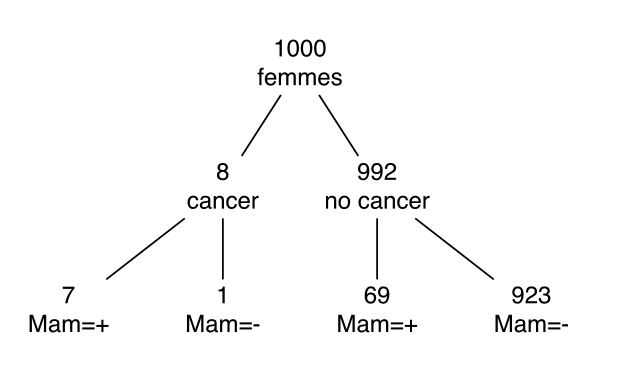
\includegraphics[width=0.5\linewidth]{figures/diagram} 

}

\caption{Diagram...}\label{fig:diagram}
\end{figure}

\[ p(Cancer = + | Mam = +) = \frac{7}{7 + 69} = \frac{7}{76} \approx .09\]

\hypertarget{diagnostique-muxe9dical-thuxe9oruxe8me-de-bayes}{%
\subsubsection{Diagnostique médical, théorème de Bayes}\label{diagnostique-muxe9dical-thuxe9oruxe8me-de-bayes}}

\[
\color{purple}{p(\theta \ | \ x)} = \dfrac{\color{orangered}{p(x \ | \ \theta)} \color{steelblue}{p(\theta)}}{\color{green}{p(x)}}
\]

\(\color{steelblue}{p(\theta)}\) { la probabilité \emph{a priori} de \(\theta\): tout ce qu'on sait de \(\theta\) avant d'observer les données. Par exemple: \(p(Cancer=+)=.008\) et \(p(Cancer=-)=.992\).}

\begin{Shaded}
\begin{Highlighting}[]
\NormalTok{prior \textless{}{-}}\StringTok{ }\KeywordTok{c}\NormalTok{(}\FloatTok{0.008}\NormalTok{, }\FloatTok{0.992}\NormalTok{)}
\end{Highlighting}
\end{Shaded}

\[
\color{purple}{p(\theta \vert x)} = \dfrac{\color{orangered}{p(x\vert \theta)} \color{steelblue}{p(\theta)}}{\color{green}{p(x)}}
\]

\(\color{orangered}{p(x\vert \theta)}\) { probabilité conditionnelle des données (\(x\)) sachant le paramètre (\(\theta\)), qu'on appelle aussi la \emph{likelihood} (\emph{ou fonction de vraisemblance}) du paramètre (\(\theta\)).}

\begin{Shaded}
\begin{Highlighting}[]
\NormalTok{like \textless{}{-}}\StringTok{ }\KeywordTok{rbind}\NormalTok{(}\KeywordTok{c}\NormalTok{(}\FloatTok{0.9}\NormalTok{, }\FloatTok{0.1}\NormalTok{), }\KeywordTok{c}\NormalTok{(}\FloatTok{0.07}\NormalTok{, }\FloatTok{0.93}\NormalTok{) ) }\OperatorTok{\%\textgreater{}\%}\StringTok{ }\NormalTok{data.frame}
\KeywordTok{colnames}\NormalTok{(like) \textless{}{-}}\StringTok{ }\KeywordTok{c}\NormalTok{(}\StringTok{"Mam+"}\NormalTok{, }\StringTok{"Mam{-}"}\NormalTok{)}
\KeywordTok{rownames}\NormalTok{(like) \textless{}{-}}\StringTok{ }\KeywordTok{c}\NormalTok{(}\StringTok{"Cancer+"}\NormalTok{, }\StringTok{"Cancer{-}"}\NormalTok{)}
\NormalTok{like}
\end{Highlighting}
\end{Shaded}

\begin{verbatim}
##         Mam+ Mam-
## Cancer+ 0.90 0.10
## Cancer- 0.07 0.93
\end{verbatim}

\[
\color{purple}{p(\theta \vert x)} = \dfrac{\color{orangered}{p(x\vert \theta)} \color{steelblue}{p(\theta)}}{\color{green}{p(x)}}
\]

{ \(p(x)\) la probabilité marginale de \(x\) (sur \(\theta\)). Sert à normaliser la distribution.}

\[\color{green}{p(x)=\sum\limits_{\theta}p(x|\theta)p(\theta)}\]

\begin{Shaded}
\begin{Highlighting}[]
\NormalTok{(marginal \textless{}{-}}\StringTok{ }\KeywordTok{sum}\NormalTok{(like}\OperatorTok{$}\StringTok{"Mam+"} \OperatorTok{*}\StringTok{ }\NormalTok{prior) )}
\end{Highlighting}
\end{Shaded}

\begin{verbatim}
## [1] 0.07664
\end{verbatim}

\[
\color{purple}{p(\theta \vert x)} = \dfrac{\color{orangered}{p(x\vert \theta)} \color{steelblue}{p(\theta)}}{\color{green}{p(x)}}
\]

\(\color{purple}{p(\theta \vert x)}\) { la probabilité a posteriori de \(\theta\) sachant \(x\), c'est à dire ce qu'on sait de \(\theta\) après avoir pris connaissance de \(x\).}

\begin{Shaded}
\begin{Highlighting}[]
\NormalTok{(posterior \textless{}{-}}\StringTok{ }\NormalTok{(like}\OperatorTok{$}\StringTok{"Mam+"} \OperatorTok{*}\StringTok{ }\NormalTok{prior ) }\OperatorTok{/}\StringTok{ }\NormalTok{marginal )}
\end{Highlighting}
\end{Shaded}

\begin{verbatim}
## [1] 0.09394572 0.90605428
\end{verbatim}

\hypertarget{linfuxe9rence-bayuxe9sienne-comme-mise-uxe0-jour-probabiliste-des-connaissances}{%
\subsubsection{L'inférence bayésienne comme mise à jour probabiliste des connaissances}\label{linfuxe9rence-bayuxe9sienne-comme-mise-uxe0-jour-probabiliste-des-connaissances}}

Avant de passer le mammogramme, la probabilité qu'une femme tirée au sort ait un cancer du sein était de \(p(Cancer)=.008\) (\emph{prior}). Après un résultat positif, cette probabilité est devenue \(p(Cancer|Mam+)=.09\) (\emph{posterior}). Ces probabilités sont des expressions de nos \emph{connaissances}. Après un mammogramme positif, on pense toujours que c'est ``très improbable'' d'avoir un cancer, mais cette probabilité a considérablement évolué relativement à ``avant le test''.

\begin{quote}
\emph{A Bayesianly justifiable analysis is one that treats known values as observed values of random variables, treats unknown values as unobserved random variables, and calculates the conditional distribution of unknowns given knowns and model specifications using Bayes' theorem} (\href{https://projecteuclid.org/euclid.aos/1176346785}{Rubin, 1984}).
\end{quote}

\hypertarget{probluxe8me-de-monty-hall}{%
\subsection{Problème de Monty Hall}\label{probluxe8me-de-monty-hall}}

\begin{figure}[!htb]

{\centering 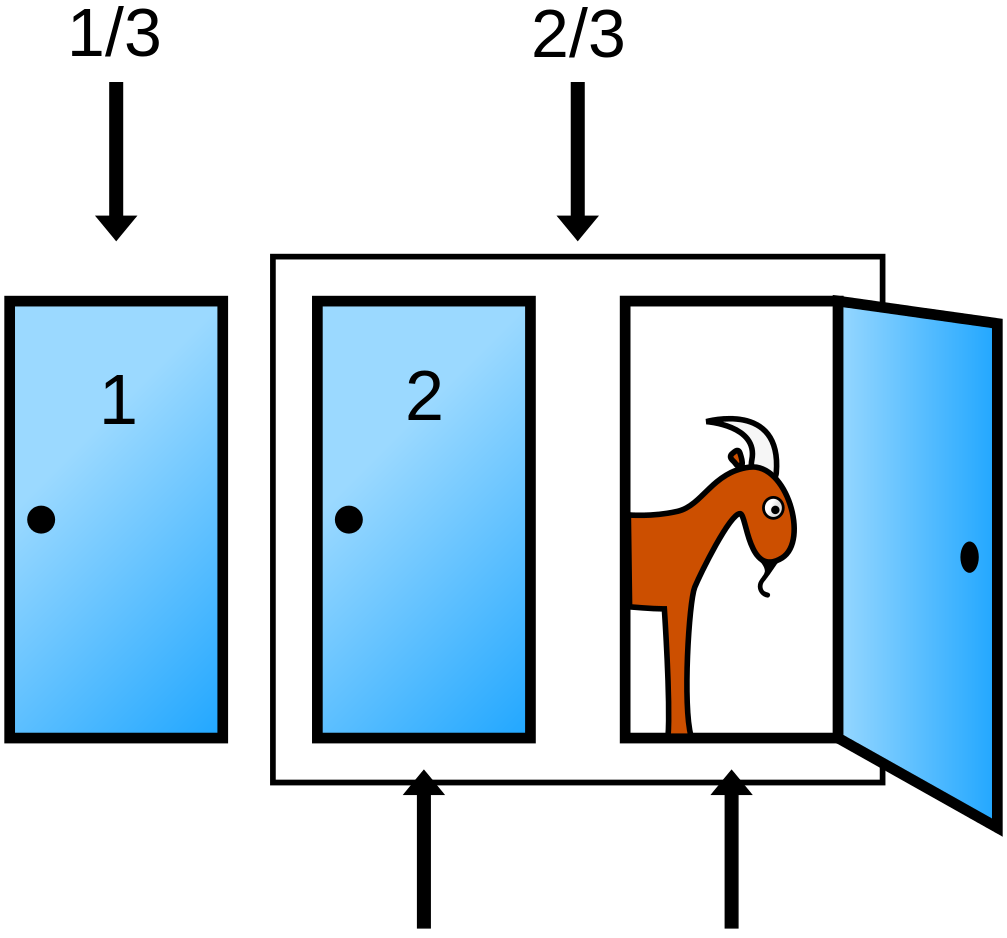
\includegraphics[width=0.5\linewidth]{figures/monty1} 

}

\caption{A syllogistic penguin... Figure from...}\label{fig:monty1}
\end{figure}

Que-feriez-vous (intuitivement) ? Analysez ensuite la situation en utilisant le théorème de Bayes.

\hypertarget{monty-hall---proposition-de-solution}{%
\subsubsection{Monty Hall - proposition de solution}\label{monty-hall---proposition-de-solution}}

Il s'agit d'un problème de probabilités conditionnelles\ldots{} Définissons les événements suivants:

P1: l'animateur ouvre la porte 1
P2: l'animateur ouvre la porte 2
P3: l'animateur ouvre la porte 3

V1: la voiture se trouve derrière la porte 1
V2: la voiture se trouve derrière la porte 2
V3: la voiture se trouve derrière la porte 3

Si on a choisi la porte n°1 et que l'animateur a choisi la porte n°3 (\emph{et qu'il sait où se trouve la voiture}), il s'ensuit que:

\(p(P3|V1)=\dfrac{1}{2}\), \(p(P3|V2)=1\), \(p(P3|V3)=0\)

On sait que \(p(V3|P3)=0\), on veut connaître \(p(V1|P3)\) et \(p(V2|P3)\) afin de pouvoir choisir. Résolution par le théorème de Bayes.

\(p(V1|P3)=\dfrac{p(P3|V1) \times p(V1)}{p(P3)}=\dfrac{\dfrac{1}{2} \times \dfrac{1}{3}}{\dfrac{1}{2}}=\dfrac{1}{3}\)

\(p(V2|P3)=\dfrac{p(P3|V2) \times p(V2)}{p(P3)}=\dfrac{1 \times \dfrac{1}{3}}{\dfrac{1}{2}}=\dfrac{2}{3}\)

\begin{figure}[!htb]

{\centering 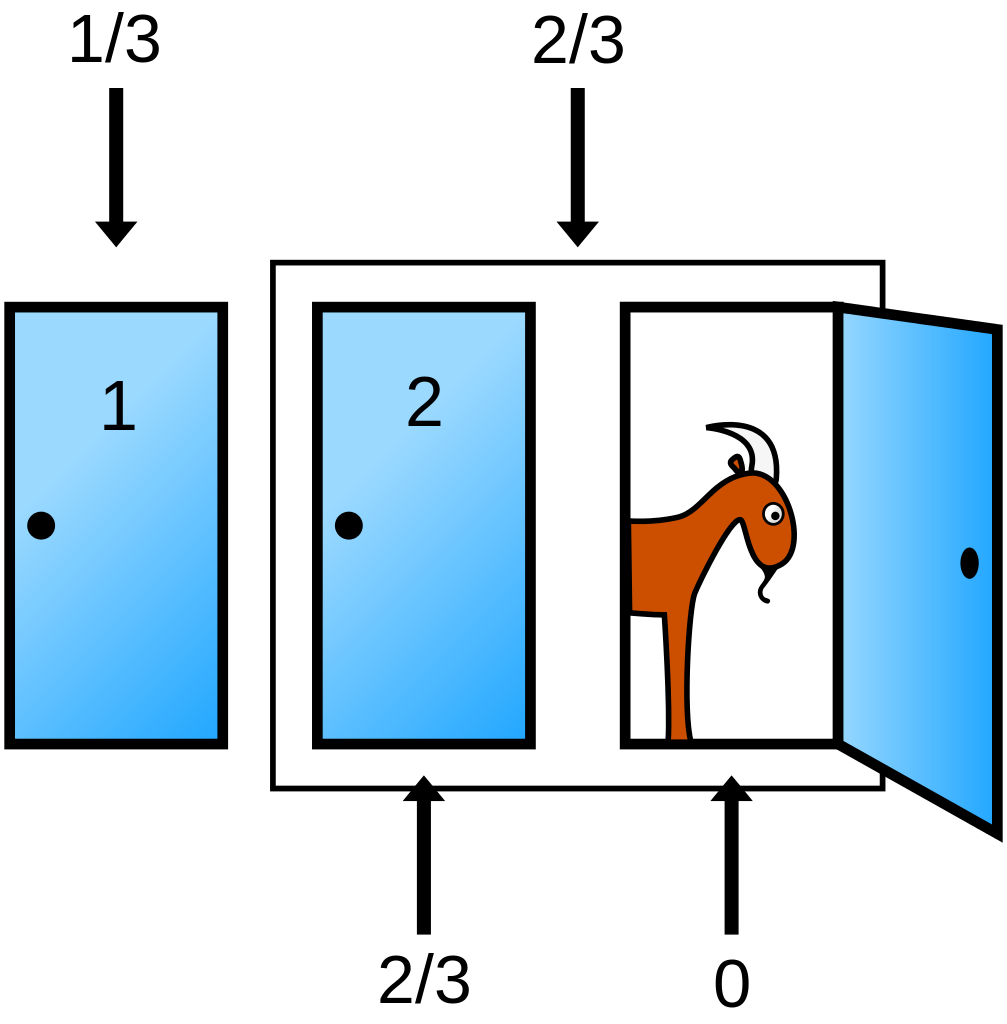
\includegraphics[width=0.5\linewidth]{figures/monty2} 

}

\caption{A syllogistic penguin... Figure from...}\label{fig:monty2}
\end{figure}

Nos intuitions probabilistes sont, dans la grande majorité des cas, très mauvaises. Au lieu de compter sur elles, il est plus sage de se reposer sur des règles logiques (\emph{modus ponens} et \emph{modus tollens}) et probabilistes simples (règle du produit, règle de la somme, théorème de Bayes), nous assurant de réaliser l'inférence logique la plus juste.

Autrement dit, ``Don't be clever'' (McElreath, \protect\hyperlink{ref-mcelreath_statistical_2016}{2016})\ldots{}

\hypertarget{beta-binomial}{%
\chapter{Modèle beta-binomial}\label{beta-binomial}}

\definecolor{steelblue}{RGB}{70, 130, 180}
\definecolor{green}{RGB}{0, 153, 0}
\definecolor{purple}{RGB}{153, 0, 153}
\definecolor{orangered}{cmyk}{0, 73, 100, 0}

Introduction au chapitre blah blah\ldots{}

\hypertarget{coefficient-binomial}{%
\section{Coefficient binomial}\label{coefficient-binomial}}

\BeginKnitrBlock{definition}[Fonction factorielle]
\protect\hypertarget{def:fonction-factorielle}{}{\label{def:fonction-factorielle} \iffalse (Fonction factorielle) \fi{} }On appelle fonction factorielle la fonction qui à tout entier naturel \(n\) associe l'entier :

\[N! = N \times (N - 1) \times (N - 2) \times \cdots \times 3 \times 2 \times 1.\]
\EndKnitrBlock{definition}

\BeginKnitrBlock{definition}[Coefficient binomial]
\protect\hypertarget{def:coefficient-binomial}{}{\label{def:coefficient-binomial} \iffalse (Coefficient binomial) \fi{} }For any nonnegative integers \(k\) and \(n\), the binomial coefficient\ldots{}
\EndKnitrBlock{definition}

\BeginKnitrBlock{theorem}[Formule du coefficient binomial]
\protect\hypertarget{thm:coefficient-binomial-formule}{}{\label{thm:coefficient-binomial-formule} \iffalse (Formule du coefficient binomial) \fi{} }For \(k \leq n\), we have:

\[
\left(\begin{array}{l}n \\ k\end{array}\right)=\frac{n(n-1) \cdots(n-k+1)}{k !}=\frac{n !}{(n-k) ! k !}
\]
For \(k > n\), we have \(\left(\begin{array}{l}n \\ k\end{array}\right) = 0\).
\EndKnitrBlock{theorem}

\begin{note}
Blah blah blah\ldots{}
\end{note}

\hypertarget{le-moduxe8le-beta-binomial}{%
\section{Le modèle Beta-Binomial}\label{le-moduxe8le-beta-binomial}}

Pourquoi ce modèle ?

Le modèle Beta-Binomial couvre un grand nombre de problèmes de la vie courante :

\begin{verbatim}
- Réussite / échec à un test
- Présence / absence d'effets secondaires lors du test d'un médicament
- Résultat d'un questionnaire à réponse binaire vrai / faux 
- Estimation des résultats du deuxième tour de l'élection présidentielle 
\end{verbatim}

C'est un modèle simple

\begin{verbatim}
- Un seul paramètre
- Solution analytique
\end{verbatim}

\hypertarget{loi-de-bernoulli}{%
\subsection{Loi de Bernoulli}\label{loi-de-bernoulli}}

S'applique à toutes les situations où le processus de génération des données ne peut résulter qu'en deux issues mutuellement exclusives (e.g., un lancer de pièce). À chaque essai, si on admet que \(\Pr(\text{face}) = \theta\), alors \(\Pr(\text{pile}) = 1 - \theta\).

Depuis Bernoulli, on sait calculer la probabilité du résultat d'un lancer de pièce, du moment que l'on connait le biais de la pièce \(\theta\). Admettons que \(Y = 0\) lorsqu'on obtient pile, et que \(Y = 1\) lorsqu'on obtient face. Alors \(Y\) est distribuée selon une loi de Bernoulli :

\[p(y) = \Pr(Y = y \ | \ \theta) = \theta^{y} (1 - \theta)^{(1 - y)}\]

En remplacant \(y\) par \(0\) ou \(1\), on retombe bien sur nos observations précédentes :

\[\Pr(Y = 0 \ | \ \theta) = \theta^{0} (1 - \theta)^{(1 - 0)} = 1 \times (1 - \theta) = 1 - \theta\]

\[\Pr(Y = 1 \ | \ \theta) = \theta^{1} (1 - \theta)^{(1 - 1)} = \theta \times 1 = \theta\]

\hypertarget{processus-de-bernoulli}{%
\subsection{Processus de Bernoulli}\label{processus-de-bernoulli}}

Si l'on dispose d'une suite de lancers \(\{Y_i\}\) indépendants et identiquement distribués (i.e., chaque lancer a une distribution de Bernoulli de probabilité \(\theta\)), l'ensemble de ces lancers peut être décrit par une \textbf{distribution binomiale}.

Par exemple, imaginons que l'on dispose de la séquence de cinq lancers suivants : Pile, Pile, Pile, Face, Face. On peut recoder cette séquence en \(\{0, 0, 0, 1, 1\}\).

Rappel : La probabilité de chaque \(1\) est \(\theta\) est la probabilité de chaque \(0\) est \(1 - \theta\).

Quelle est la probabilité d'obtenir 2 faces sur 5 lancers ?

\hypertarget{processus-de-bernoulli-1}{%
\subsection{Processus de Bernoulli}\label{processus-de-bernoulli-1}}

Sachant que les essais sont indépendants les uns des autres, la probabilité d'obtenir cette séquence est de \((1 - \theta) \times (1 - \theta) \times (1 - \theta) \times \theta \times \theta\), c'est à dire : \(\theta^{2} (1 - \theta)^{3}\).

On peut généraliser ce résultat pour une séquence de \(n\) lancers et \(y\) ``succès'' :

\[\theta^{y} (1 - \theta)^{n - y}\]

Mais, jusque là on a considéré seulement une seule séquence résultant en 2 succès pour 5 lancers, mais il existe de nombreuses séquences pouvant résulter en 2 succès pour 5 lancers (e.g., \(\{0, 0, 1, 0, 1\}\))\ldots{}

\hypertarget{coefficient-binomial-1}{%
\subsection{Coefficient binomial}\label{coefficient-binomial-1}}

Le \textbf{coefficient binomial} nous permet de calculer le nombre d'arrangements possibles résultant en \(y\) succès pour \(n\) lancers de la manière suivante :

\[
\left(\begin{array}{l} n \\ y \end{array}\right) = C_{n}^{y} = \frac{n !}{y !(n - y) !}
\]

Par exemple pour \(y = 1\) et \(n = 3\), on sait qu'il existe 3 arrangements possibles : \(\{0, 0, 1\}, \{0, 1, 0\}, \{1, 0, 0\}\). On peut vérifier ça par le calcul, en appliquant la formule ci-dessus.

\[
\left(\begin{array}{l} 3 \\ 1\end{array}\right) = C_{1}^{3} = \frac{3 !}{1 !(3 - 1) !} = \frac{6}{2} = 3
\]

\begin{Shaded}
\begin{Highlighting}[]
\CommentTok{\# computing the total number of possible arrangements in R}
\KeywordTok{choose}\NormalTok{(}\DataTypeTok{n =} \DecValTok{3}\NormalTok{, }\DataTypeTok{k =} \DecValTok{1}\NormalTok{)}
\end{Highlighting}
\end{Shaded}

\begin{verbatim}
## [1] 3
\end{verbatim}

\hypertarget{loi-binomiale}{%
\subsection{Loi binomiale}\label{loi-binomiale}}

\[
p(y \ | \ \theta) = \Pr(Y = y \ | \ \theta) = \left(\begin{array}{l} n \\ y \end{array}\right) \theta^{y}(1 - \theta)^{n - y}
\]

La loi binomiale nous permet de calculer la probabilité d'obtenir \(y\) succès sur \(n\) essais, pour un \(\theta\) donné. Exemple de la distribution binomiale pour une pièce non biaisée (\(\theta = 0.5\)), indiquant la probabilité d'obtenir \(n\) faces sur 10 lancers (en R: \texttt{dbinom(x\ =\ 0:10,\ size\ =\ 10,\ prob\ =\ 0.5)}).

\begin{figure}[!htb]

{\centering 
\includegraphics[width=0.75\linewidth]{IMSB_files/figure-latex/binomial-barplot2-1} 

}

\caption{Binomial distribution barplot...}\label{fig:binomial-barplot2}
\end{figure}

\hypertarget{guxe9nuxe9rer-des-donnuxe9es-uxe0-partir-dune-distribution-binomiale}{%
\subsection{Générer des données à partir d'une distribution binomiale}\label{guxe9nuxe9rer-des-donnuxe9es-uxe0-partir-dune-distribution-binomiale}}

\begin{Shaded}
\begin{Highlighting}[]
\KeywordTok{library}\NormalTok{(tidyverse)}
\KeywordTok{set.seed}\NormalTok{(}\DecValTok{666}\NormalTok{) }\CommentTok{\# for reproducibility}

\KeywordTok{rbinom}\NormalTok{(}\DataTypeTok{n =} \DecValTok{500}\NormalTok{, }\DataTypeTok{size =} \DecValTok{1}\NormalTok{, }\DataTypeTok{prob =} \FloatTok{0.6}\NormalTok{) }\OperatorTok{\%\textgreater{}\%}\StringTok{ }\CommentTok{\# theta = 0.6}
\StringTok{        }\NormalTok{data.frame }\OperatorTok{\%\textgreater{}\%}
\StringTok{        }\KeywordTok{mutate}\NormalTok{(}\DataTypeTok{x =} \KeywordTok{seq\_along}\NormalTok{(.), }\DataTypeTok{y =} \KeywordTok{cumsum}\NormalTok{(.) }\OperatorTok{/}\StringTok{ }\KeywordTok{seq\_along}\NormalTok{(.) ) }\OperatorTok{\%\textgreater{}\%}
\StringTok{        }\KeywordTok{ggplot}\NormalTok{(}\KeywordTok{aes}\NormalTok{(}\DataTypeTok{x =}\NormalTok{ x, }\DataTypeTok{y =}\NormalTok{ y), }\DataTypeTok{log =} \StringTok{"y"}\NormalTok{) }\OperatorTok{+}
\StringTok{        }\KeywordTok{geom\_line}\NormalTok{(}\DataTypeTok{lwd =} \DecValTok{1}\NormalTok{) }\OperatorTok{+}
\StringTok{        }\KeywordTok{geom\_hline}\NormalTok{(}\DataTypeTok{yintercept =} \FloatTok{0.5}\NormalTok{, }\DataTypeTok{lty =} \DecValTok{3}\NormalTok{) }\OperatorTok{+}
\StringTok{        }\KeywordTok{xlab}\NormalTok{(}\StringTok{"Nombre de lancers"}\NormalTok{) }\OperatorTok{+}
\StringTok{        }\KeywordTok{ylab}\NormalTok{(}\StringTok{"Proportion de faces"}\NormalTok{) }\OperatorTok{+}
\StringTok{        }\KeywordTok{ylim}\NormalTok{(}\DecValTok{0}\NormalTok{, }\DecValTok{1}\NormalTok{) }\OperatorTok{+}
\StringTok{        }\KeywordTok{theme\_bw}\NormalTok{(}\DataTypeTok{base\_size =} \DecValTok{18}\NormalTok{)}
\end{Highlighting}
\end{Shaded}

\begin{figure}[!htb]

{\centering 
\includegraphics[width=0.75\linewidth]{IMSB_files/figure-latex/berndata-1} 

}

\caption{Long-run...}\label{fig:berndata}
\end{figure}

\hypertarget{duxe9finition-du-moduxe8le-likelihood}{%
\subsection{Définition du modèle (likelihood)}\label{duxe9finition-du-moduxe8le-likelihood}}

\hypertarget{fonction-de-vraisemblance-likelihood}{%
\subsubsection{Fonction de vraisemblance (likelihood)}\label{fonction-de-vraisemblance-likelihood}}

\begin{itemize}
\tightlist
\item
  Nous considérons \(y\) comme étant le nombre de succès
\item
  Nous considérons le nombre d'observations \(n\) comme étant une \textbf{constante}
\item
  Nous considérons \(\theta\) comme étant le \textbf{paramètre} de notre modèle (i.e., la probabilité de succès)
\end{itemize}

La fonction de vraisemblance s'écrit de la manière suivante :

\[
\color{orangered}{\mathcal{L}(\theta\ |\ y, n) = p(y \ |\ \theta, n) = \left(\begin{array}{l} n \\ y \end{array}\right) \theta^{y}(1 - \theta)^{n - y} \propto \theta^{y}(1 - \theta)^{n - y}}
\]

\hypertarget{vraisemblance-versus-probabilituxe9}{%
\subsection{Vraisemblance versus probabilité}\label{vraisemblance-versus-probabilituxe9}}

On lance à nouveau une pièce de biais \(\theta\) (où \(\theta\) représente la probabilité d'obtenir Face). On lance cette pièce deux fois et on obtient une Face et un Pile.

On peut calculer la probabilité de ces données selon (i.e., \emph{en fonction de}) différentes valeurs de \(\theta\) de la manière suivante :

\[
\begin{aligned}
\Pr(F, P \ | \ \theta) + \Pr(P, F \ | \ \theta) &= \theta(1 - \theta) + \theta(1 - \theta) \\
&= 2 \times \Pr(P \ | \ \theta) \times \Pr(F \ | \ \theta) \\
&= 2 \theta(1 - \theta)
\end{aligned}
\]

Cette probabilité est définie pour un jeu de données fixe et une valeur de \(\theta\) variable. On peut représenter cette fonction visuellement. Représentation graphique de la fonction de vraisemblance de theta pour x = 1 et n = 2\ldots{}

\begin{Shaded}
\begin{Highlighting}[]
\NormalTok{y \textless{}{-}}\StringTok{ }\DecValTok{1} \CommentTok{\# number of heads}
\NormalTok{n \textless{}{-}}\StringTok{ }\DecValTok{2} \CommentTok{\# number of trials}

\KeywordTok{data.frame}\NormalTok{(}\DataTypeTok{theta =} \KeywordTok{seq}\NormalTok{(}\DataTypeTok{from =} \DecValTok{0}\NormalTok{, }\DataTypeTok{to =} \DecValTok{1}\NormalTok{, }\DataTypeTok{length.out =} \FloatTok{1e3}\NormalTok{) ) }\OperatorTok{\%\textgreater{}\%}
\StringTok{  }\KeywordTok{mutate}\NormalTok{(}\DataTypeTok{likelihood =} \KeywordTok{dbinom}\NormalTok{(}\DataTypeTok{x =}\NormalTok{ y, }\DataTypeTok{size =}\NormalTok{ n, }\DataTypeTok{prob =}\NormalTok{ theta) ) }\OperatorTok{\%\textgreater{}\%}
\StringTok{  }\KeywordTok{ggplot}\NormalTok{(}\KeywordTok{aes}\NormalTok{(}\DataTypeTok{x =}\NormalTok{ theta, }\DataTypeTok{y =}\NormalTok{ likelihood) ) }\OperatorTok{+}
\StringTok{  }\KeywordTok{geom\_area}\NormalTok{(}\DataTypeTok{color =} \StringTok{"orangered"}\NormalTok{, }\DataTypeTok{fill =} \StringTok{"orangered"}\NormalTok{, }\DataTypeTok{alpha =} \FloatTok{0.5}\NormalTok{) }\OperatorTok{+}
\StringTok{  }\KeywordTok{xlab}\NormalTok{(}\KeywordTok{expression}\NormalTok{(}\KeywordTok{paste}\NormalTok{(theta, }\StringTok{" {-} Pr(face)"}\NormalTok{) ) ) }\OperatorTok{+}\StringTok{ }\KeywordTok{ylab}\NormalTok{(}\StringTok{"Likelihod"}\NormalTok{) }\OperatorTok{+}
\StringTok{  }\KeywordTok{theme\_bw}\NormalTok{(}\DataTypeTok{base\_size =} \DecValTok{20}\NormalTok{)}
\end{Highlighting}
\end{Shaded}

\begin{figure}[!htb]

{\centering 
\includegraphics[width=0.75\linewidth]{IMSB_files/figure-latex/likelihood-1} 

}

\caption{Likelihood plot...}\label{fig:likelihood}
\end{figure}

Si on calcule l'aire sous la courbe de cette fonction, on obtient :

\[\int_{0}^{1} 2 \theta(1 - \theta) \mathrm{d} \theta = \frac{1}{3}\]

\begin{Shaded}
\begin{Highlighting}[]
\NormalTok{f \textless{}{-}}\StringTok{ }\ControlFlowTok{function}\NormalTok{(theta) \{}\DecValTok{2} \OperatorTok{*}\StringTok{ }\NormalTok{theta }\OperatorTok{*}\StringTok{ }\NormalTok{(}\DecValTok{1} \OperatorTok{{-}}\StringTok{ }\NormalTok{theta) \}}
\KeywordTok{integrate}\NormalTok{(}\DataTypeTok{f =}\NormalTok{ f, }\DataTypeTok{lower =} \DecValTok{0}\NormalTok{, }\DataTypeTok{upper =} \DecValTok{1}\NormalTok{)}
\end{Highlighting}
\end{Shaded}

\begin{verbatim}
## 0.3333333 with absolute error < 3.7e-15
\end{verbatim}

Quand on varie \(\theta\), la fonction de vraisemblance \emph{n'est pas} une distribution de probabilité valide (i.e., son intégrale n'est pas égale à 1). On utilise le terme de \textbf{vraisemblance}, pour distinguer ce type de fonction des fonctions de densité de probabilité. On utilise la notation suivante pour mettre l'accent sur le fait que la fonction de vraisemblance est une fonction de \(\theta\), et que les données sont fixes : \(\mathcal{L}(\theta \ | \ data) = p(data \ | \ \theta)\).

Notons que la vraisemblance de \(\theta\) pour une donnée particulière est égale à la probabilité de cette donnée pour cette valeur de \(\theta\). Cependant, la \emph{distribution} de ces vraisemblances (en colonne) n'est pas une distribution de probabilités. Dans l'analyse bayésienne, \textbf{les données sont considérées comme fixes} et la valeur de \(\theta\) est considérée comme une \textbf{variable aléatoire}.

\hypertarget{duxe9finition-du-prior}{%
\subsection{Définition du prior}\label{duxe9finition-du-prior}}

Comment définir un prior dans le cas du lancer de pièce ?

\textbf{Aspect sémantique} \(~\rightarrow~\) \emph{doit pouvoir rendre compte} :
+ D'une absence d'information
+ D'une connaissance d'observations antérieures concernant la pièce étudiée
+ D'un niveau d'incertitude concernant ces observations antérieures

\textbf{Aspect mathématique} \(~\rightarrow~\) \emph{pour une solution entièrement analytique} :
+ Les distributions a priori et a posteriori doivent avoir la même forme
+ La vraisemblance marginale doit pouvoir se calculer analytiquement

\hypertarget{la-distribution-beta}{%
\subsection{La distribution Beta}\label{la-distribution-beta}}

\[
\begin{aligned}
\color{steelblue}{p(\theta\ | \ a, b)} \ &\color{steelblue}{= \mathrm{Beta}(\theta\ |\ a, b)} \\
& \color{steelblue}{= \theta^{a - 1}(1 - \theta)^{b - 1} / B(a, b)} \\
& \color{steelblue}{\propto \theta^{a - 1}(1 - \theta)^{b - 1}}
\end{aligned}
\]

où \(a\) et \(b\) sont deux paramètres tels que \(a \geq 0\), \(b \geq 0\), et \(B(a, b)\) est une constante de normalisation.

\begin{figure}[!htb]

{\centering 
\includegraphics[width=0.75\linewidth]{IMSB_files/figure-latex/beta1-1} 

}

\caption{Distribution Beta...}\label{fig:beta1}
\end{figure}

\hypertarget{interpruxe9tation-des-paramuxe8tres-du-prior-beta}{%
\subsection{Interprétation des paramètres du prior Beta}\label{interpruxe9tation-des-paramuxe8tres-du-prior-beta}}

\begin{itemize}
\tightlist
\item
  On peut exprimer l'absence de connaissance a priori par \(a = b = 1\) (distribution orange)
\item
  On peut exprimer un prior en faveur d'une absence de biais par \(a = b > 2\) (distribution verte)
\item
  On peut exprimer un biais en faveur de \emph{Face} par \(a > b\) (distribution bleue)
\item
  On peut exprimer un biais en faveur de \emph{Pile} par \(a < b\) (distribution violette)
\end{itemize}

\begin{figure}[!htb]

{\centering 
\includegraphics[width=0.75\linewidth]{IMSB_files/figure-latex/beta2-1} 

}

\caption{Inteprétation des paramètres d'une distribution Beta.}\label{fig:beta2}
\end{figure}

Le niveau de certitude augmente avec la somme \(\kappa = a + b\)

\begin{itemize}
\tightlist
\item
  Aucune idée sur la provenance de la pièce : \(a = b = 1\) -\textgreater{} \textbf{prior plat}
\item
  En attendant le début de l'expérience, on a lancé la pièce 10 fois et observé 5 ``Face'' : \(a = b = 5\) -\textgreater{} \textbf{prior peu informatif}
\item
  La pièce provient de la banque de France : \(a = b = 50\) -\textgreater{} \textbf{prior fort}
\end{itemize}

\begin{figure}[!htb]

{\centering 
\includegraphics[width=0.75\linewidth]{IMSB_files/figure-latex/beta3-1} 

}

\caption{Interprétation des paramètres d'une distribution Beta...}\label{fig:beta3}
\end{figure}

Supposons que l'on dispose d'une estimation de la valeur la plus probable \(\omega\) du paramètre \(\theta\). On peut reparamétriser la distribution Beta en fonction du mode \(\omega\) et du niveau de certitude \(\kappa\) :

\[
\begin{aligned}
a &= \omega(\kappa - 2) + 1 \\
b &= (1 - \omega)(\kappa - 2) + 1 &&\mbox{pour } \kappa > 2
\end{aligned}
\]

Si \(\omega = 0.65\) et \(\kappa = 25\) alors \(p(\theta) = \mathrm{Beta}(\theta \ | \ 15.95, 9.05)\).
Si \(\omega = 0.65\) et \(\kappa = 10\) alors \(p(\theta) = \mathrm{Beta}(\theta \ | \ 6.2, 3.8)\).

\begin{figure}[!htb]

{\centering 
\includegraphics[width=0.75\linewidth]{IMSB_files/figure-latex/beta4-1} 

}

\caption{Blah blah...}\label{fig:beta4}
\end{figure}

\hypertarget{prior-conjuguuxe9}{%
\subsection{Prior conjugué}\label{prior-conjuguuxe9}}

Formellement, si \(\mathcal{F}\) est une classe de distributions d'échantillonnage \(p(y|\theta)\), et \(\mathcal{P}\) est une classe de distributions a priori pour \(\theta\), alors \(\mathcal{P}\) est \textbf{conjuguée} à \(\mathcal{F}\) si et seulement si :

\[
p(\theta|y) \in \mathcal{P} \text{ for all } p(\cdot | \theta) \in \mathcal{F} \text{ and } p(\cdot) \in \mathcal{P}
\]

(Gelman et al., 2013, p.35). En d'autres termes, un prior est appelé \textbf{conjugué} si, lorsqu'il est converti en une distribution a posteriori en étant multiplié par la vraisemblance, il conserve la même forme. Dans notre cas, le prior Beta est un prior conjugué pour la vraisemblance binomiale, car le posterior est également une distribution Beta.

\begin{quote}
Le résultat du produit d'un prior Beta et d'une fonction de vraisemblance Binomiale est proportionnel à une distribution Beta. On dit alors que la distribution Beta est \textbf{un prior conjugué} de la fonction de vraisemblance Binomiale.
\end{quote}

\hypertarget{duxe9rivation-analytique-de-la-distribution-a-posteriori}{%
\subsection{Dérivation analytique de la distribution a posteriori}\label{duxe9rivation-analytique-de-la-distribution-a-posteriori}}

Soit un prior défini par : \(\ \color{steelblue}{p(\theta \ | \ a, b) = \mathrm{Beta}(a, b) \propto \theta^{a - 1}(1 - \theta)^{b - 1}}\)

Soit une fonction de vraisemblance associée à \(y\) ``Face'' pour \(n\) lancers : \(\ \color{orangered}{p(y \ | \ n, \theta) = \mathrm{Bin}(y \ | \ n, \theta) = \left(\begin{array}{l} n \\ y \end{array}\right) \theta^{y}(1 - \theta)^{n - y} \propto \theta^{y}(1 - \theta)^{n - y}}\)

\[
\begin{aligned}
\color{purple}{p(\theta \ | \ y, n)} &\propto \color{orangered}{p(y \ | \ n, \theta)} \ \color{steelblue}{p(\theta)} &&\mbox{Théorème de Bayes} \\
&\propto \color{orangered}{\mathrm{Bin}(y \ | \ n, \theta)} \ \color{steelblue}{\mathrm{Beta}(\theta \ | \ a, b)} \\
&\propto \color{orangered}{\theta^{y}(1 - \theta)^{n - y}} \ \color{steelblue}{\theta^{a - 1}(1 - \theta)^{b - 1}} &&\mbox{Application des formules précédentes} \\
&\propto \color{purple}{\theta}^{\color{orangered}{y} + \color{steelblue}{a - 1}}\color{purple}{(1 - \theta)}^{\color{orangered}{n - y} + \color{steelblue}{b - 1}} &&\mbox{En regroupant les termes identiques} \\
&\propto \color{purple}{\theta^{a' - 1}(1 - \theta)^{b' - 1}} &&\mbox{Avec } a' = y + a \mbox{ et } b' = n - y + b \\
\color{purple}{p(\theta \ | \ y, n)} \ &= \color{purple}{\mathrm{Beta}(y + a, n - y + b)}
\end{aligned}
\]

\hypertarget{un-exemple-pour-diguxe9rer}{%
\subsection{Un exemple pour digérer}\label{un-exemple-pour-diguxe9rer}}

On observe \(y = 7\) réponses correctes sur \(n = 10\) questions. On choisit un prior \(\mathrm{Beta}(1, 1)\), c'est à dire un prior uniforme sur \([0, 1]\). Ce prior équivaut à une connaissance a priori de 0 succès et 0 échecs (i.e., prior plat).

La distribution postérieure est donnée par :

\[
\begin{aligned}
\color{purple}{p(\theta \ | \ y, n)} &\propto \color{orangered}{p(y \ | \ n, \theta)} \ \color{steelblue}{p(\theta)} \\
&\propto \color{orangered}{\mathrm{Bin}(7 \ | \ 10, \theta)} \ \color{steelblue}{\mathrm{Beta}(\theta \ | \ 1, 1)} \\
&= \color{purple}{\mathrm{Beta}(y + a, n - y + b)} \\
&= \color{purple}{\mathrm{Beta}(8, 4)}
\end{aligned}
\]

La moyenne de la distribution postérieure est donnée par :

\[
\color{purple}{\underbrace{\frac{y + a}{n + a + b}}_{posterior}} = \color{orangered}{\underbrace{\frac{y}{n}}_{data}} \underbrace{\frac{n}{n + a + b}}_{weight} + \color{steelblue}{\underbrace{\frac{a}{a + b}}_{prior}} \underbrace{\frac{a + b}{n + a + b}}_{weight}
\]

Blah blah\ldots{}

\begin{figure}[!htb]

{\centering 
\includegraphics[width=0.75\linewidth]{IMSB_files/figure-latex/beta-exemple-1} 

}

\caption{Exemple...}\label{fig:beta-exemple}
\end{figure}

\hypertarget{influence-du-prior-sur-la-distribution-postuxe9rieure}{%
\subsection{Influence du prior sur la distribution postérieure}\label{influence-du-prior-sur-la-distribution-postuxe9rieure}}

Cas \(n < a + b, (n = 10, a = 4, b = 16)\).

\begin{figure}[!htb]

{\centering 
\includegraphics[width=0.75\linewidth]{IMSB_files/figure-latex/posterior-exemple1-1} 

}

\caption{Influence du prior...}\label{fig:posterior-exemple1}
\end{figure}

Cas \(n = a + b, (n = 20, a = 4, b = 16)\).

\begin{figure}[!htb]

{\centering 
\includegraphics[width=0.75\linewidth]{IMSB_files/figure-latex/posterior-exemple2-1} 

}

\caption{Influence du prior...}\label{fig:posterior-exemple2}
\end{figure}

Cas \(n > a + b, (n = 40, a = 4, b = 16)\).

\begin{figure}[!htb]

{\centering 
\includegraphics[width=0.75\linewidth]{IMSB_files/figure-latex/posterior-exemple3-1} 

}

\caption{Influence du prior...}\label{fig:posterior-exemple3}
\end{figure}

\hypertarget{ce-quil-faut-retenir}{%
\subsection{Ce qu'il faut retenir}\label{ce-quil-faut-retenir}}

\begin{quote}
The posterior distribution is always a compromise between the prior distribution and the likelihood function.
\emph{Kruschke (2015)}
\end{quote}

\begin{figure}[!htb]

{\centering 
\includegraphics[width=0.75\linewidth]{IMSB_files/figure-latex/posterior-exemple4-1} 

}

\caption{Influence du prior...}\label{fig:posterior-exemple4}
\end{figure}

Plus on a de données, moins le prior a d'influence dans l'estimation de la distribution a posteriori (et réciproquement).

Attention : Lorsque le prior accorde une probabilité de 0 à certaines valeurs de \(\theta\), le modèle est incapable d'apprendre (ces valeurs sont alors considérées comme ``impossibles'')\ldots{}

\begin{figure}[!htb]

{\centering 
\includegraphics[width=0.75\linewidth]{IMSB_files/figure-latex/posterior-exemple5-1} 

}

\caption{Influence du prior...}\label{fig:posterior-exemple5}
\end{figure}

\hypertarget{la-vraisemblance-marginale-the-devil-is-in-the-denominator}{%
\subsection{La vraisemblance marginale (the devil is in the denominator)}\label{la-vraisemblance-marginale-the-devil-is-in-the-denominator}}

\[
Posterior = \frac{Likelihood \ \times \ Prior}{Marginal \ Likelihood} \propto Likelihood \ \times \ Prior
\]

\[
p(\theta \ | \ data) = \frac{p(data \ | \ \theta) \ \times \ p(\theta)}{p(data)} \propto p(data \ | \ \theta) \ \times \ p(\theta)
\]

Si on zoom sur la vraisemblance marginale (aussi connue comme \emph{evidence})\ldots{}

\[
\begin{aligned}
\color{green}{p(data)} &= \int p(data,\theta) \, \mathrm d\theta &&\text{Marginalisation sur le paramètre } \theta \\
\color{green}{p(data)} &= \color{green}{\int p(data \ | \ \theta) \ p(\theta) \, \mathrm{d} \theta} && \text{Application de la règle du produit}
\end{aligned}
\]

Petit problème : \(p(data)\) se calcule en calculant la somme (pour des variables discrètes) ou l'intégrale (pour des variables continues) de la densité conjointe \(p(data, \theta)\) sur toutes les valeurs possibles de \(\theta\). Cela se complique lorsque le modèle comprend plusieurs paramètres.

Par exemple pour deux paramètres discrets :

\[
p(data) = \sum_{\theta_{1}} \sum_{\theta_{2}} p(data, \theta_{1}, \theta_{2})
\]

Et pour un modèle avec deux paramètres continus :

\[
p(data) = \int\limits_{\theta_{1}} \int\limits_{\theta_{2}} p(data, \theta_{1}, \theta_{2}) \mathrm{d} \theta_{1} \mathrm{d} \theta_{2}
\]

Trois méthodes pour résoudre (contourner) ce problème :

\begin{enumerate}
\def\labelenumi{\arabic{enumi}.}
\item
  Solution analytique \(~\longrightarrow~\) Utilisation d'un prior conjugué (e.g., le modèle Beta-Binomial)
\item
  Solution discrètisée \(~\longrightarrow~\) Calcul de la solution sur un ensemble fini de points (grid method)
\item
  Solution approchée \(~\longrightarrow~\) On échantillonne ``intelligemment'' l'espace conjoint des paramètres (méthodes MCMC, cf.~cours n°05)
\end{enumerate}

\hypertarget{la-distribution-postuxe9rieure-solution-analytique}{%
\subsection{La distribution postérieure, solution analytique}\label{la-distribution-postuxe9rieure-solution-analytique}}

\hypertarget{distributions-discruxe8tes}{%
\subsubsection{Distributions discrètes}\label{distributions-discruxe8tes}}

\begin{figure}[!htb]

{\centering 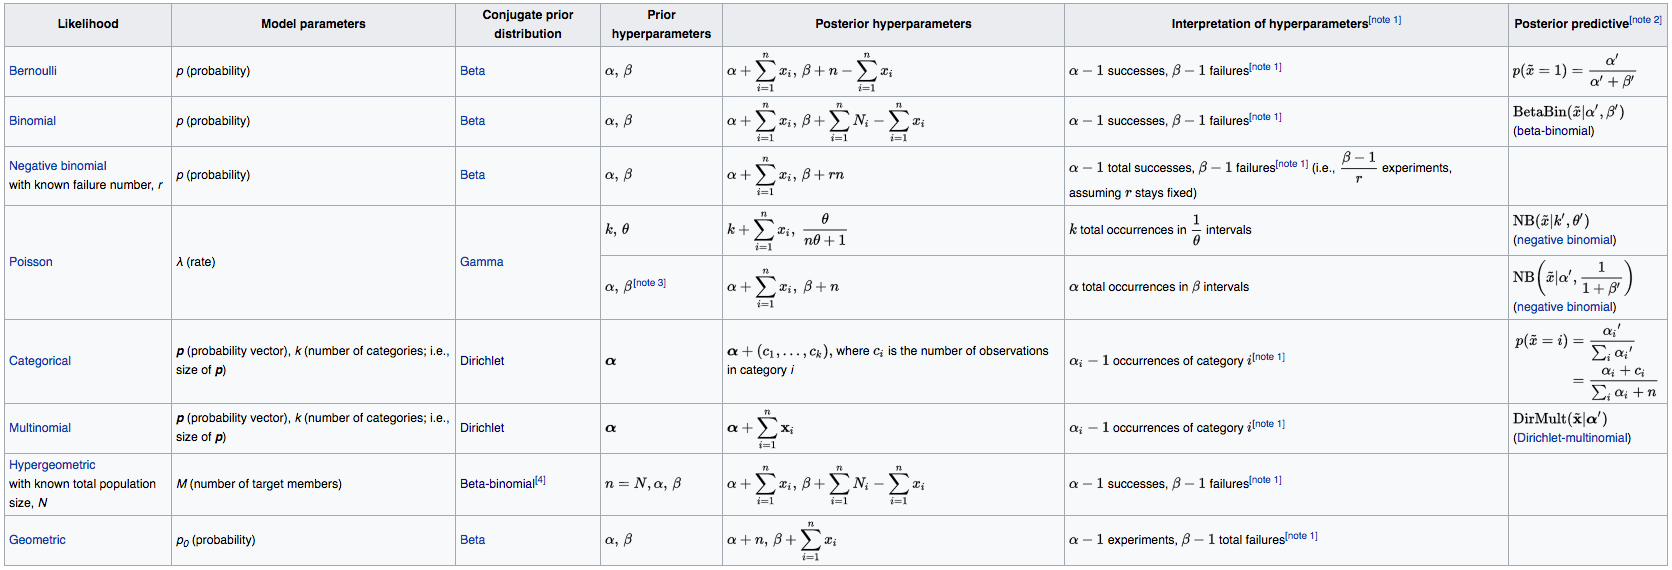
\includegraphics[width=1\linewidth]{figures/discrete} 

}

\caption{Illustration of the Mersenne-Twister algorithm... Figure from...}\label{fig:discrete}
\end{figure}

\hypertarget{distributions-continues}{%
\subsubsection{Distributions continues}\label{distributions-continues}}

\begin{figure}[!htb]

{\centering 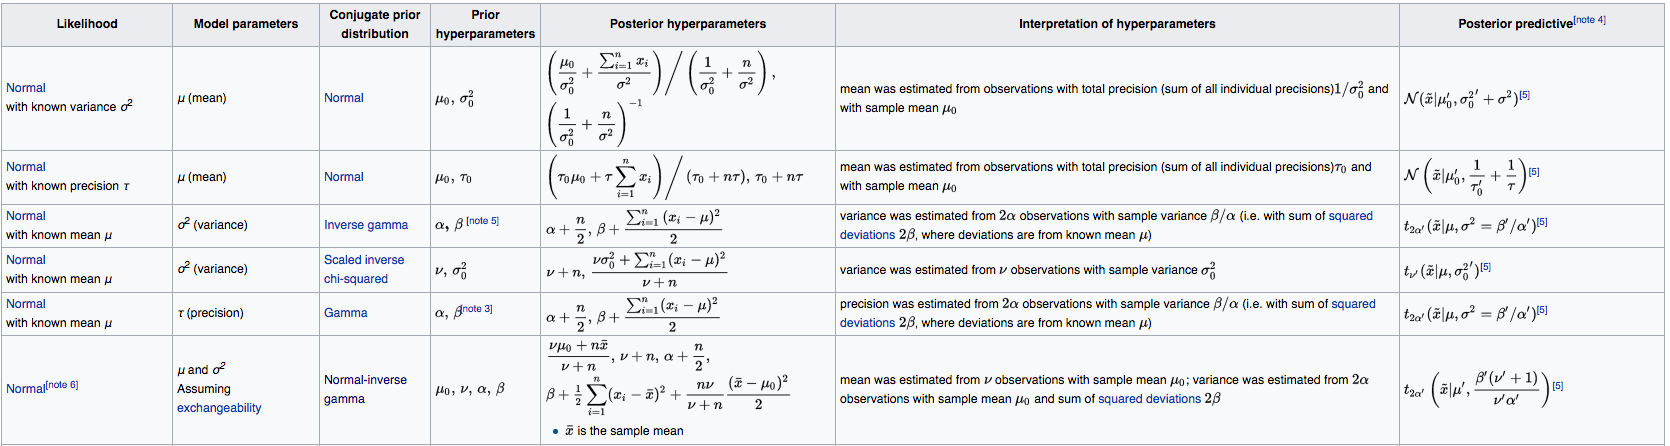
\includegraphics[width=1\linewidth]{figures/continuous} 

}

\caption{Illustration of the Mersenne-Twister algorithm... Figure from...}\label{fig:continuous}
\end{figure}

Problème : Cette solution est très contraignante. Idéalement, le modèle (likelihood + prior) devrait être défini à partir de l'interprétation que l'on peut faire des paramètres de ces distributions, et non pour faciliter les calculs\ldots{}

\hypertarget{la-distribution-postuxe9rieure-grid-method}{%
\subsection{La distribution postérieure, grid method}\label{la-distribution-postuxe9rieure-grid-method}}

\begin{enumerate}
\def\labelenumi{\arabic{enumi}.}
\tightlist
\item
  \textbf{Définir la grille}
\item
  Calculer la valeur du prior pour chaque valeur de la grille
\item
  Calculer la valeur de la vraisemblance pour chaque valeur de la grille
\item
  Calculer le produit prior x vraisemblance pour chaque valeur de la grille, puis normalisation du résultat
\end{enumerate}

\begin{figure}[!htb]

{\centering 
\includegraphics[width=0.75\linewidth]{IMSB_files/figure-latex/grid1-1} 

}

\caption{Blah blah...}\label{fig:grid1}
\end{figure}

\begin{enumerate}
\def\labelenumi{\arabic{enumi}.}
\tightlist
\item
  Définir la grille
\item
  \textbf{Calculer la valeur du prior pour chaque valeur de la grille}
\item
  Calculer la valeur de la vraisemblance pour chaque valeur de la grille
\item
  Calculer le produit prior x vraisemblance pour chaque valeur de la grille, puis normalisation du résultat
\end{enumerate}

\begin{figure}[!htb]

{\centering 
\includegraphics[width=0.75\linewidth]{IMSB_files/figure-latex/grid2-1} 

}

\caption{Blah blah...}\label{fig:grid2}
\end{figure}

\begin{enumerate}
\def\labelenumi{\arabic{enumi}.}
\tightlist
\item
  Définir la grille
\item
  Calculer la valeur du prior pour chaque valeur de la grille
\item
  \textbf{Calculer la valeur de la vraisemblance pour chaque valeur de la grille}
\item
  Calculer le produit prior x vraisemblance pour chaque valeur de la grille, puis normalisation du résultat
\end{enumerate}

\begin{figure}[!htb]

{\centering 
\includegraphics[width=0.75\linewidth]{IMSB_files/figure-latex/grid3-1} 

}

\caption{Blah blah...}\label{fig:grid3}
\end{figure}

\begin{enumerate}
\def\labelenumi{\arabic{enumi}.}
\tightlist
\item
  Définir la grille
\item
  Calculer la valeur du prior pour chaque valeur de la grille
\item
  Calculer la valeur de la vraisemblance pour chaque valeur de la grille
\item
  \textbf{Calculer le produit prior x vraisemblance pour chaque valeur de la grille, puis normalisation du résultat}
\end{enumerate}

\begin{figure}[!htb]

{\centering 
\includegraphics[width=0.75\linewidth]{IMSB_files/figure-latex/grid4-1} 

}

\caption{Blah blah...}\label{fig:grid4}
\end{figure}

\begin{enumerate}
\def\labelenumi{\arabic{enumi}.}
\tightlist
\item
  Définir la grille
\item
  Calculer la valeur du prior pour chaque valeur de la grille
\item
  Calculer la valeur de la vraisemblance pour chaque valeur de la grille
\item
  \textbf{Calculer le produit prior x vraisemblance pour chaque valeur de la grille, puis normalisation du résultat}
\end{enumerate}

\begin{figure}[!htb]

{\centering 
\includegraphics[width=0.75\linewidth]{IMSB_files/figure-latex/grid5-1} 

}

\caption{Blah blah...}\label{fig:grid5}
\end{figure}

Problème du nombre de paramètres\ldots{} En affinant la grille on augmente le temps de calcul :

\begin{itemize}
\tightlist
\item
  3 paramètres avec une grille de \(10^3\) noeuds = une grille de \(10^9\) points de calcul
\item
  10 paramètres avec une grille de \(10^3\) noeuds = une grille de \(10^{30}\) points de calcul
\end{itemize}

Le ``superordinateur'' chinois Tianhe-2 réalise \(33,8 \text{×} 10^{15}\) opérations par seconde. Si on considère qu'il réalise 3 opérations par noeud de la grille, il lui faudrait \(10^{14}\) secondes pour parcourir la grille une fois (pour comparaison, l'âge de l'univers est approximativement de \((4,354 ± 0,012)\text{×}10^{17}\) secondes)\ldots{}

\hypertarget{uxe9chantillonner-la-distribution-postuxe9rieure}{%
\subsection{Échantillonner la distribution postérieure}\label{uxe9chantillonner-la-distribution-postuxe9rieure}}

Pour échantillonner une distribution postérieure, on peut utiliser une approximation par grille ou différentes implémentations des méthodes MCMC (e.g., Metropolis-Hasting, Gibbs, Hamilton, cf.~Cours n°05).

En pratique :

\begin{Shaded}
\begin{Highlighting}[]
\NormalTok{p\_grid \textless{}{-}}\StringTok{ }\KeywordTok{seq}\NormalTok{(}\DataTypeTok{from =} \DecValTok{0}\NormalTok{, }\DataTypeTok{to =} \DecValTok{1}\NormalTok{, }\DataTypeTok{length.out =} \DecValTok{1000}\NormalTok{) }\CommentTok{\# creating a grid}
\NormalTok{prior \textless{}{-}}\StringTok{ }\KeywordTok{rep}\NormalTok{(}\DecValTok{1}\NormalTok{, }\DecValTok{1000}\NormalTok{) }\CommentTok{\# uniform prior}
\NormalTok{likelihood \textless{}{-}}\StringTok{ }\KeywordTok{dbinom}\NormalTok{(y, }\DataTypeTok{size =}\NormalTok{ n, }\DataTypeTok{prob =}\NormalTok{ p\_grid) }\CommentTok{\# computes likelihood}
\NormalTok{posterior \textless{}{-}}\StringTok{ }\NormalTok{(likelihood }\OperatorTok{*}\StringTok{ }\NormalTok{prior) }\OperatorTok{/}\StringTok{ }\KeywordTok{sum}\NormalTok{(likelihood }\OperatorTok{*}\StringTok{ }\NormalTok{prior) }\CommentTok{\# computes posterior}
\NormalTok{samples \textless{}{-}}\StringTok{ }\KeywordTok{sample}\NormalTok{(posterior, }\DataTypeTok{size =} \FloatTok{1e3}\NormalTok{, }\DataTypeTok{prob =}\NormalTok{ posterior, }\DataTypeTok{replace =} \OtherTok{TRUE}\NormalTok{) }\CommentTok{\# sampling}
\KeywordTok{hist}\NormalTok{(samples, }\DataTypeTok{main =} \StringTok{""}\NormalTok{, }\DataTypeTok{xlab =} \KeywordTok{expression}\NormalTok{(theta), }\DataTypeTok{cex.axis =} \DecValTok{1}\NormalTok{, }\DataTypeTok{cex.lab =} \FloatTok{1.5}\NormalTok{) }\CommentTok{\# histogram}
\end{Highlighting}
\end{Shaded}

\begin{figure}[!htb]

{\centering 
\includegraphics[width=0.75\linewidth]{IMSB_files/figure-latex/sampling1-1} 

}

\caption{Blah blah...}\label{fig:sampling1}
\end{figure}

La précision dépend de la taille de l'échantillon\ldots{}

\begin{figure}[!htb]

{\centering 
\includegraphics[width=0.75\linewidth]{IMSB_files/figure-latex/sampling2-1} 

}

\caption{Blah blah...}\label{fig:sampling2}
\end{figure}

\begin{figure}[!htb]

{\centering 
\includegraphics[width=0.75\linewidth]{IMSB_files/figure-latex/sampling3-1} 

}

\caption{Blah blah...}\label{fig:sampling3}
\end{figure}

\hypertarget{la-distribution-postuxe9rieure-ruxe9sumuxe9}{%
\subsection{La distribution postérieure, résumé}\label{la-distribution-postuxe9rieure-ruxe9sumuxe9}}

\begin{itemize}
\tightlist
\item
  Cas analytique :
\end{itemize}

\begin{Shaded}
\begin{Highlighting}[]
\NormalTok{p\_grid \textless{}{-}}\StringTok{ }\KeywordTok{seq}\NormalTok{(}\DataTypeTok{from =} \DecValTok{0}\NormalTok{, }\DataTypeTok{to =} \DecValTok{1}\NormalTok{, }\DataTypeTok{length.out =} \DecValTok{1000}\NormalTok{)}
\NormalTok{a \textless{}{-}}\StringTok{ }\NormalTok{b \textless{}{-}}\StringTok{ }\DecValTok{1} \CommentTok{\# parameters of the Beta prior}
\NormalTok{n \textless{}{-}}\StringTok{ }\DecValTok{9} \CommentTok{\# number of observations}
\NormalTok{y \textless{}{-}}\StringTok{ }\DecValTok{6} \CommentTok{\# number of successes}
\NormalTok{posterior \textless{}{-}}\StringTok{ }\KeywordTok{dbeta}\NormalTok{(p\_grid, z }\OperatorTok{+}\StringTok{ }\NormalTok{a }\OperatorTok{{-}}\StringTok{ }\DecValTok{1}\NormalTok{, N }\OperatorTok{{-}}\StringTok{ }\NormalTok{z }\OperatorTok{+}\StringTok{ }\NormalTok{b }\OperatorTok{{-}}\StringTok{ }\DecValTok{1}\NormalTok{)}
\end{Highlighting}
\end{Shaded}

\begin{itemize}
\tightlist
\item
  Grid method :
\end{itemize}

\begin{Shaded}
\begin{Highlighting}[]
\NormalTok{p\_grid \textless{}{-}}\StringTok{ }\KeywordTok{seq}\NormalTok{( }\DataTypeTok{from =} \DecValTok{0}\NormalTok{, }\DataTypeTok{to =} \DecValTok{1}\NormalTok{, }\DataTypeTok{length.out =} \DecValTok{1000}\NormalTok{)}
\NormalTok{prior \textless{}{-}}\StringTok{ }\KeywordTok{rep}\NormalTok{(}\DecValTok{1}\NormalTok{, }\DecValTok{1000}\NormalTok{) }\CommentTok{\# uniform prior}
\NormalTok{likelihood \textless{}{-}}\StringTok{ }\KeywordTok{dbinom}\NormalTok{(y, }\DataTypeTok{size =}\NormalTok{ n, }\DataTypeTok{prob =}\NormalTok{ p\_grid)}
\NormalTok{posterior \textless{}{-}}\StringTok{ }\NormalTok{(likelihood }\OperatorTok{*}\StringTok{ }\NormalTok{prior) }\OperatorTok{/}\StringTok{ }\KeywordTok{sum}\NormalTok{(likelihood }\OperatorTok{*}\StringTok{ }\NormalTok{prior)}
\end{Highlighting}
\end{Shaded}

\begin{itemize}
\tightlist
\item
  Échantillonner la distribution postérieure :
\end{itemize}

\begin{Shaded}
\begin{Highlighting}[]
\KeywordTok{sample}\NormalTok{(data, }\DataTypeTok{size =}\NormalTok{ trajLength, }\DataTypeTok{prob =}\NormalTok{ prob, }\DataTypeTok{replace =} \OtherTok{TRUE}\NormalTok{)}
\end{Highlighting}
\end{Shaded}

\textbf{Méthode analytique}
* La distribution postérieure est décrite explicitement
* Le modèle est fortement contraint

\textbf{Méthode Grid}
* La distribution postérieure n'est donnée que pour un ensemble fini de valeurs
* Plus la grille est fine, meilleure est l'estimation de la distribution postérieure
* Compromis \emph{Précision - Temps de calcul}

\hypertarget{utiliser-les-uxe9chantillons-pour-ruxe9sumer-la-distribution-postuxe9rieure}{%
\subsection{Utiliser les échantillons pour résumer la distribution postérieure}\label{utiliser-les-uxe9chantillons-pour-ruxe9sumer-la-distribution-postuxe9rieure}}

\hypertarget{estimation-de-la-tendance-centrale}{%
\subsubsection{Estimation de la tendance centrale}\label{estimation-de-la-tendance-centrale}}

À partir d'un ensemble d'échantillons d'une distribution postérieure, on peut calculer la moyenne, le mode, et la médiane. Par exemple pour un prior uniforme, 10 lancers et 3 Faces.

\begin{Shaded}
\begin{Highlighting}[]
\NormalTok{mode\_posterior \textless{}{-}}\StringTok{ }\KeywordTok{find\_mode}\NormalTok{(samples) }\CommentTok{\# in blue}
\NormalTok{mean\_posterior \textless{}{-}}\StringTok{ }\KeywordTok{mean}\NormalTok{(samples) }\CommentTok{\# in orange}
\NormalTok{median\_posterior \textless{}{-}}\StringTok{ }\KeywordTok{median}\NormalTok{(samples) }\CommentTok{\# in green}
\end{Highlighting}
\end{Shaded}

\begin{figure}[!htb]

{\centering 
\includegraphics[width=0.75\linewidth]{IMSB_files/figure-latex/tendance-centrale2-1} 

}

\caption{Blah blah...}\label{fig:tendance-centrale2}
\end{figure}

Quelle est la probabilité que le biais de la pièce \(\theta\) soit supérieur à 0.5 ?

\begin{Shaded}
\begin{Highlighting}[]
\KeywordTok{sum}\NormalTok{(samples }\OperatorTok{\textgreater{}}\StringTok{ }\FloatTok{0.5}\NormalTok{) }\OperatorTok{/}\StringTok{ }\KeywordTok{length}\NormalTok{(samples) }\CommentTok{\# length(samples) is the number of samples}
\end{Highlighting}
\end{Shaded}

\begin{verbatim}
## [1] 0.1152
\end{verbatim}

Quelle est la probabilité que le biais de la pièce \(\theta\) soit compris entre 0.2 et 0.4 ?

\begin{Shaded}
\begin{Highlighting}[]
\KeywordTok{sum}\NormalTok{(samples }\OperatorTok{\textgreater{}}\StringTok{ }\FloatTok{0.2} \OperatorTok{\&}\StringTok{ }\NormalTok{samples }\OperatorTok{\textless{}}\StringTok{ }\FloatTok{0.4}\NormalTok{) }\OperatorTok{/}\StringTok{ }\FloatTok{1e4} \CommentTok{\# length(samples) is the number of samples}
\end{Highlighting}
\end{Shaded}

\begin{verbatim}
## [1] 0.5547
\end{verbatim}

\begin{figure}[!htb]

{\centering 
\includegraphics[width=0.75\linewidth]{IMSB_files/figure-latex/interval-prob-plot-1} 

}

\caption{Blah blah...}\label{fig:interval-prob-plot}
\end{figure}

\hypertarget{highest-density-interval-hdi}{%
\subsection{Highest density interval (HDI)}\label{highest-density-interval-hdi}}

\begin{itemize}
\tightlist
\item
  Le HDI indique les valeurs du paramètre qui sont les plus probables (sachant les données et le prior)
\item
  Plus le HDI est étroit et plus le degré de certitude est élevé
\item
  La largeur du HDI diminue avec l'augmentation du nombre de mesures
\end{itemize}

\begin{quote}
Définition: les valeurs du paramètre \(\theta\) contenues dans un HDI à 89\% sont telles que \(p(\theta) > W\) où \(W\) satisfait la condition suivante :

\[\int_{\theta \ : \ p(\theta) > W} p(\theta) \, \mathrm{d} \theta = 0.89.\]
\end{quote}

\begin{figure}[!htb]

{\centering 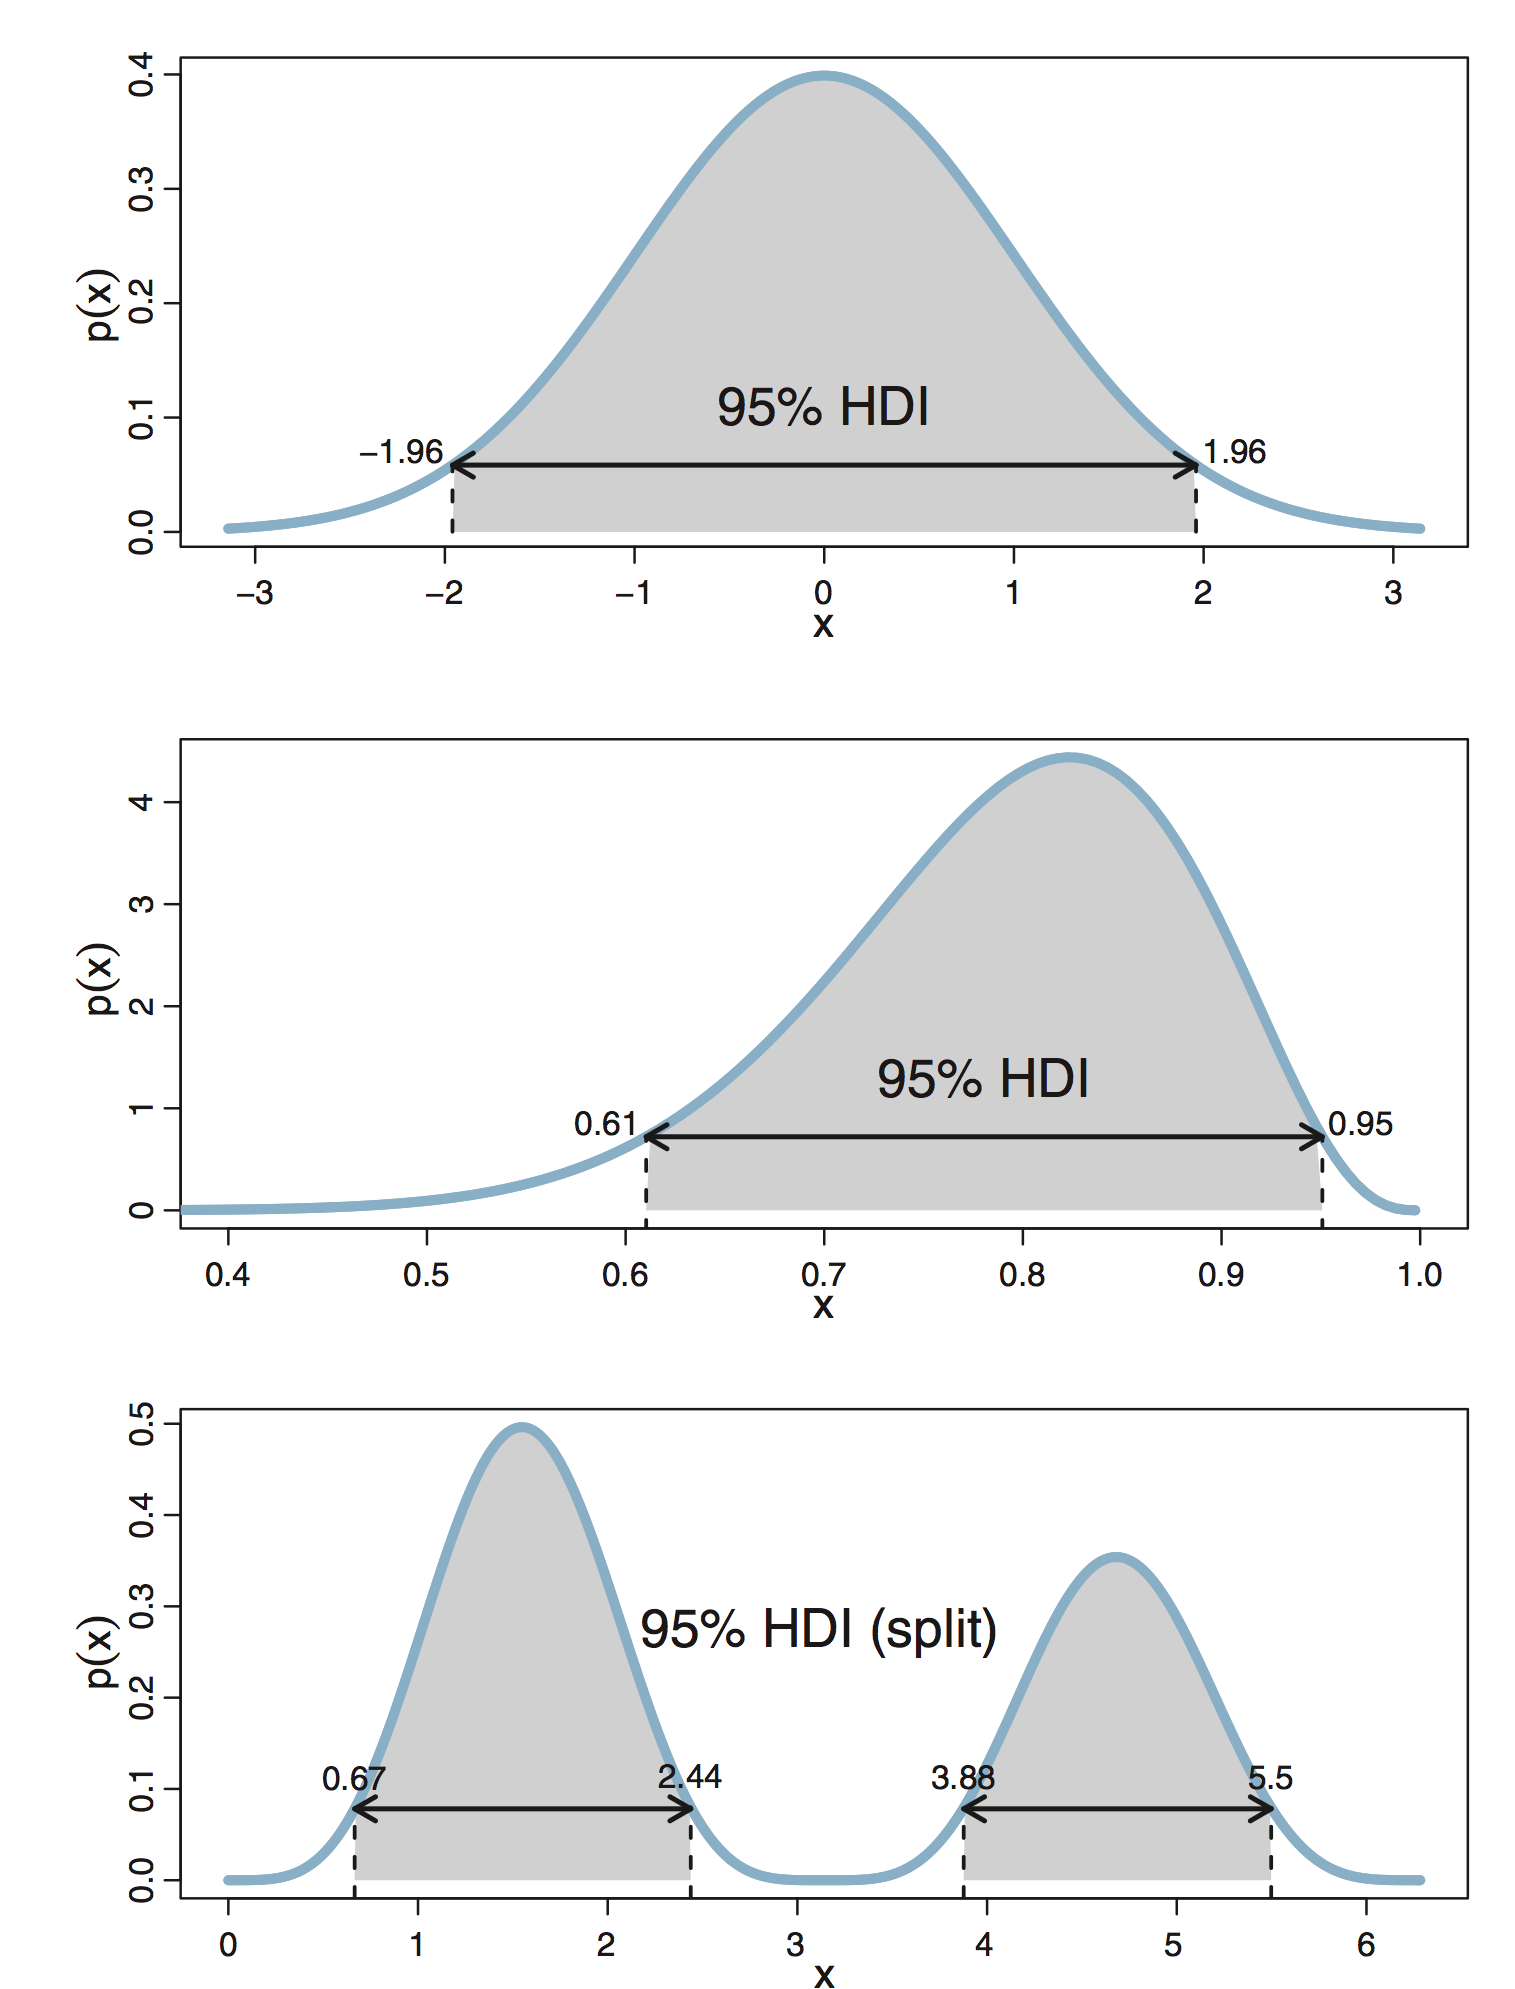
\includegraphics[width=1\linewidth]{figures/HDI} 

}

\caption{Illustration of the Mersenne-Twister algorithm... Figure from...}\label{fig:hdi}
\end{figure}

\begin{Shaded}
\begin{Highlighting}[]
\KeywordTok{library}\NormalTok{(BEST)}

\KeywordTok{set.seed}\NormalTok{(}\DecValTok{666}\NormalTok{)}
\NormalTok{p\_grid \textless{}{-}}\StringTok{ }\KeywordTok{seq}\NormalTok{(}\DataTypeTok{from =} \DecValTok{0}\NormalTok{, }\DataTypeTok{to =} \DecValTok{1}\NormalTok{, }\DataTypeTok{length.out =} \FloatTok{1e3}\NormalTok{)}
\NormalTok{pTheta \textless{}{-}}\StringTok{ }\KeywordTok{dbeta}\NormalTok{(p\_grid, }\DecValTok{3}\NormalTok{, }\DecValTok{10}\NormalTok{)}
\NormalTok{massVec \textless{}{-}}\StringTok{ }\NormalTok{pTheta }\OperatorTok{/}\StringTok{ }\KeywordTok{sum}\NormalTok{(pTheta)}
\NormalTok{samples \textless{}{-}}\StringTok{ }\KeywordTok{sample}\NormalTok{(p\_grid, }\DataTypeTok{size =} \FloatTok{1e4}\NormalTok{, }\DataTypeTok{replace =} \OtherTok{TRUE}\NormalTok{, }\DataTypeTok{prob =}\NormalTok{ pTheta)}

\KeywordTok{plotPost}\NormalTok{(samples, }\DataTypeTok{credMass =} \FloatTok{0.89}\NormalTok{, }\DataTypeTok{cex =} \FloatTok{1.5}\NormalTok{, }\DataTypeTok{xlab =} \KeywordTok{expression}\NormalTok{(theta), }\DataTypeTok{xlim =} \KeywordTok{c}\NormalTok{(}\DecValTok{0}\NormalTok{, }\DecValTok{1}\NormalTok{) )}
\end{Highlighting}
\end{Shaded}

\begin{figure}[!htb]

{\centering 
\includegraphics[width=0.75\linewidth]{IMSB_files/figure-latex/plotpost1-1} 

}

\caption{Blah blah...}\label{fig:plotpost1}
\end{figure}

\hypertarget{region-of-practical-equivalence-rope}{%
\subsection{Region of practical equivalence (ROPE)}\label{region-of-practical-equivalence-rope}}

On l'utilise pour tester une hypothèse :

\begin{itemize}
\tightlist
\item
  La valeur du paramètre (e.g., \(\theta = 0.5\)) est rejetée si le HDI est entièrement hors de la ROPE
\item
  La valeur du paramètre (e.g., \(\theta = 0.5\)) est acceptée si le HDI est entièrement dans la ROPE
\item
  Si le HDI et la ROPE se chevauchent on ne peut pas conclure\ldots{}
\end{itemize}

\begin{figure}[!htb]

{\centering 
\includegraphics[width=0.75\linewidth]{IMSB_files/figure-latex/rope-1} 

}

\caption{Blah blah...}\label{fig:rope}
\end{figure}

\hypertarget{comparaison-de-moduxe8les}{%
\subsection{Comparaison de modèles}\label{comparaison-de-moduxe8les}}

On lance une pièce 200 fois et on obtient 115 \emph{Faces}\ldots{} est-ce que la pièce est biaisée ? Nous construisons deux modèles et essayons de savoir lequel rend le mieux compte des données.

\[
\begin{aligned}
\mathcal{M}_0: Y &\sim \mathrm{Binomial}(n, \theta = 0.5) && \text{La pièce n'est pas biaisée}\\
\mathcal{M}_1: Y &\sim \mathrm{Binomial}(n, \theta \neq 0.5) && \text{La pièce est biaisée}
\end{aligned}
\]

Le facteur de Bayes (\emph{Bayes factor}) fait le rapport des vraisemblances (marginales) des deux modèles.

\[
\frac{p(\mathcal{M}_{0} \ | \ data)}{p(\mathcal{M}_{1} \ | \ data)} = \color{green}{\frac{p(data \ | \ \mathcal{M}_{0})}{p(data \ | \ \mathcal{M}_{1})}} \ \frac{p(\mathcal{M}_{0})}{p(\mathcal{M}_{1})}
\]

Soit dans notre exemple :

\[
BF_{01} = \frac{p(\mathcal{M}_{0} \ | \ data)}{p(\mathcal{M}_{1} \ | \ data)} = \frac{0.005955}{0.005} = 1.1971.
\]

Le rapport de probabilités a augmenté de 20\% en faveur de \(\mathcal{M}_{0}\) après avoir pris connaissance des données.

\hypertarget{model-checking}{%
\subsection{Model checking}\label{model-checking}}

Les deux rôles de la fonction de vraisemblance :

\begin{itemize}
\tightlist
\item
  C'est une fonction de \(\theta\) pour le calcul de la distribution postérieure : \(\mathcal{L}(\theta \ | \ y, n)\)
\item
  Lorsque \(\theta\) est connu / fixé, c'est une distribution de probabilité : \(p(y \ |\ \theta, n) = \theta^y(1 - \theta)^{(n - y)}\)
\end{itemize}

On peut utiliser cette distribution de probabilité pour générer des données\ldots{} !

Par exemple : Générer 10000 valeurs à partir d'une loi binomiale basée sur 9 lancers et une probabilité de Face de 0.6 :

\begin{Shaded}
\begin{Highlighting}[]
\NormalTok{samples \textless{}{-}}\StringTok{ }\KeywordTok{rbinom}\NormalTok{(}\DataTypeTok{n =} \FloatTok{1e4}\NormalTok{, }\DataTypeTok{size =} \DecValTok{10}\NormalTok{, }\DataTypeTok{prob =} \FloatTok{0.6}\NormalTok{)}
\end{Highlighting}
\end{Shaded}

Deux sources d'incertitude dans ces prédictions :

\begin{itemize}
\tightlist
\item
  Incertitude liée au processus d'échantillonnage
  -\textgreater{} Chaque valeur apparaît avec une probabilité \(\theta\)
\item
  Incertitude sur la valeur de \(\theta\) elle-même
  -\textgreater{} Pour chaque valeur de \(\theta\) on peut calculer une distribution implicite
\end{itemize}

Par exemple : Générer 10000 valeurs à partir d'une loi binomiale basé sur 9 lancers et une probabilité de Face décrite par la distribution postérieure de \(\theta\) :

\begin{Shaded}
\begin{Highlighting}[]
\NormalTok{samples \textless{}{-}}\StringTok{ }\KeywordTok{rbinom}\NormalTok{(}\DataTypeTok{n =} \FloatTok{1e4}\NormalTok{, }\DataTypeTok{size =} \DecValTok{10}\NormalTok{, }\DataTypeTok{prob =} \KeywordTok{rbeta}\NormalTok{(}\FloatTok{1e4}\NormalTok{, }\DecValTok{16}\NormalTok{, }\DecValTok{10}\NormalTok{) )}
\end{Highlighting}
\end{Shaded}

\hypertarget{posterior-predictive-checking}{%
\subsection{Posterior predictive checking}\label{posterior-predictive-checking}}

\begin{figure}[!htb]

{\centering 
\includegraphics[width=0.75\linewidth]{IMSB_files/figure-latex/ppc-1} 

}

\caption{Blah blah...}\label{fig:ppc}
\end{figure}

Blah blah\ldots{}

\begin{figure}[!htb]

{\centering 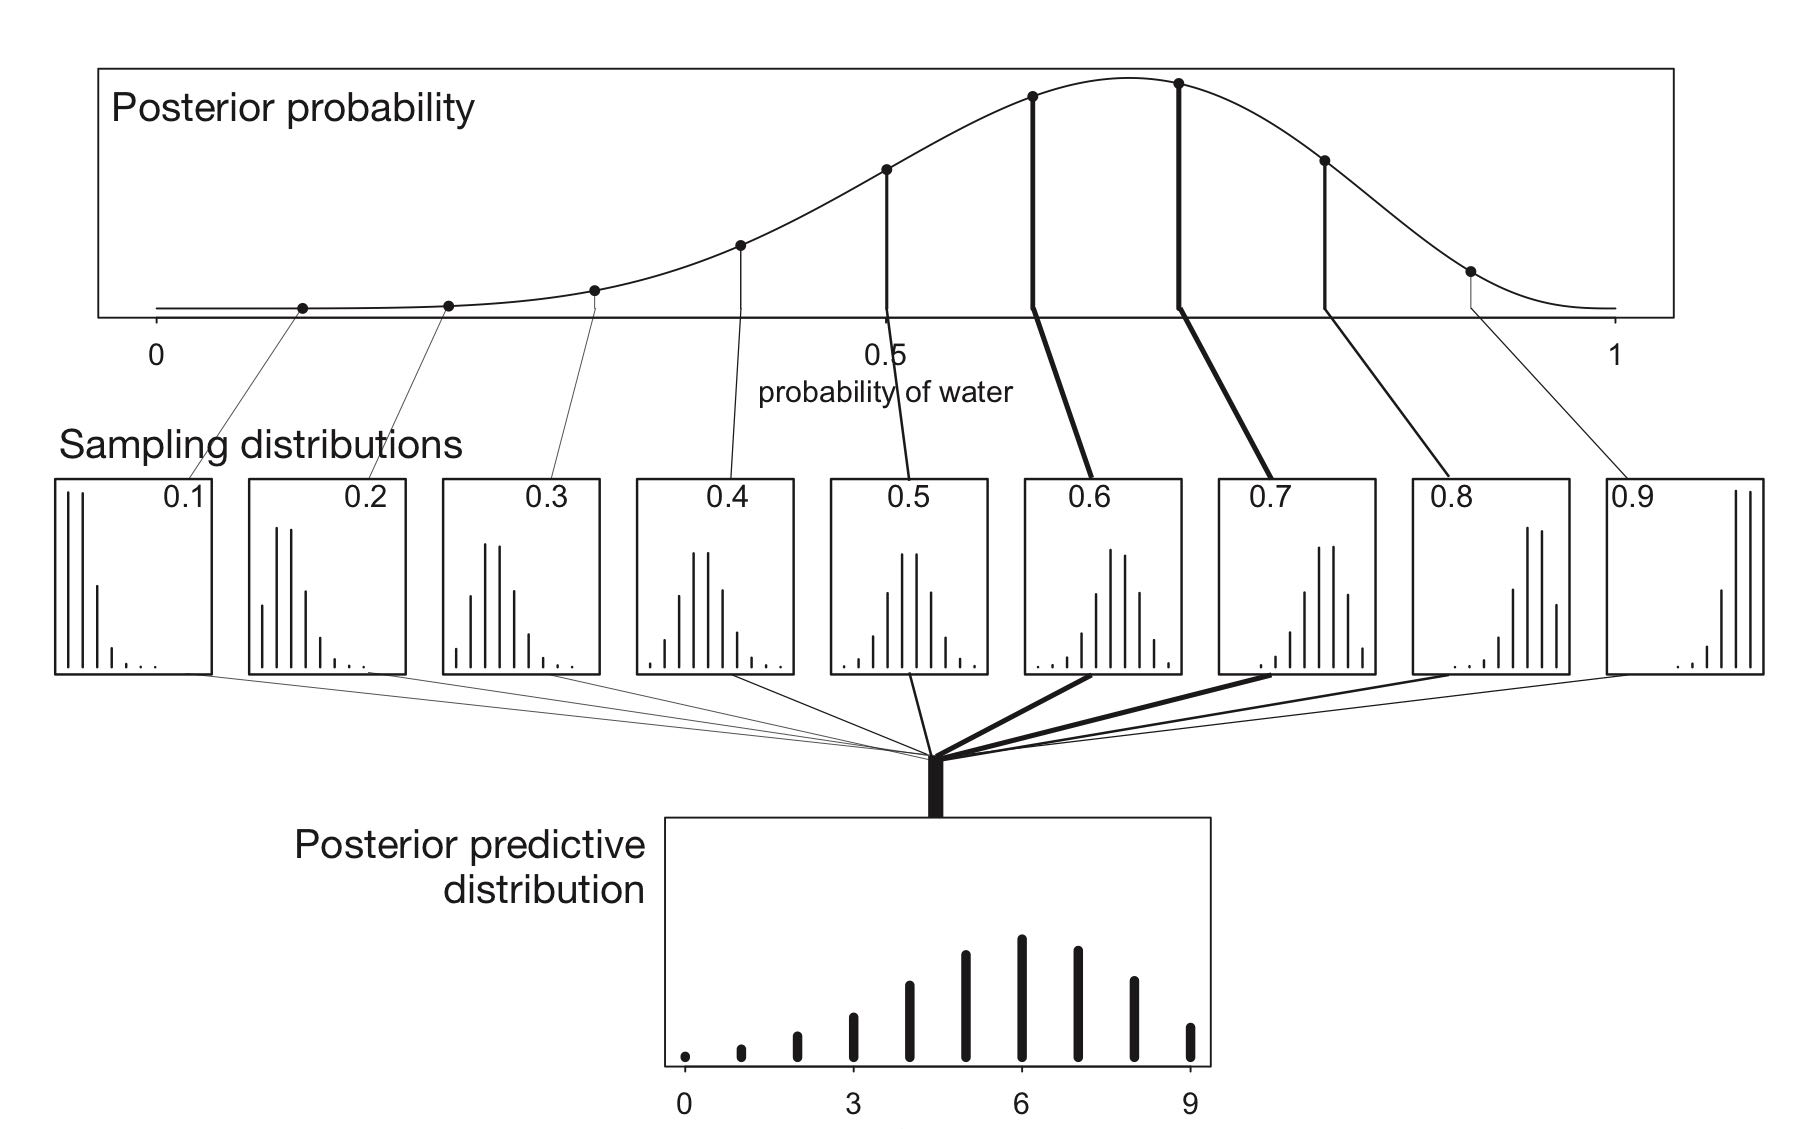
\includegraphics[width=1\linewidth]{figures/ModelPredictions} 

}

\caption{Illustration of the posterior predictive checking procedure. Figure from McElreath (2016).}\label{fig:ppc-rethinking}
\end{figure}

\hypertarget{conclusions}{%
\section{Conclusions}\label{conclusions}}

\ldots{}

\hypertarget{linear-regression1}{%
\chapter{Modèle de régression linéaire}\label{linear-regression1}}

\definecolor{steelblue}{RGB}{70, 130, 180}
\definecolor{green}{RGB}{0, 153, 0}
\definecolor{purple}{RGB}{153, 0, 153}
\definecolor{orangered}{cmyk}{0, 73, 100, 0}

Introduction au chapitre blah blah\ldots{}

\hypertarget{langage-de-la-moduxe9lisation}{%
\section{Langage de la modélisation}\label{langage-de-la-moduxe9lisation}}

\[
\begin{aligned}
y_{i} &\sim \mathrm{Normal}(\mu_{i}, \sigma) \\
\mu_{i}&= \alpha + \beta x_{i} \\
\alpha &\sim \mathrm{Normal}(60, 10) \\
\beta &\sim \mathrm{Normal}(0, 10) \\
\sigma &\sim \mathrm{HalfCauchy}(0, 1)
\end{aligned}
\]

\textbf{Objectif de la séance} : comprendre ce type de modèle.

Les constituants de nos modèles seront toujours les mêmes et nous suivrons les deux mêmes étapes :

\begin{itemize}
\tightlist
\item
  Construire le modèle (\emph{likelihood} + \emph{priors}).
\item
  Mettre à jour grâce aux données (\emph{updating}), afin de calculer la distribution postérieure.
\end{itemize}

\hypertarget{un-premier-moduxe8le}{%
\section{Un premier modèle}\label{un-premier-moduxe8le}}

\begin{Shaded}
\begin{Highlighting}[]
\KeywordTok{library}\NormalTok{(rethinking)}
\KeywordTok{library}\NormalTok{(tidyverse)}

\KeywordTok{data}\NormalTok{(Howell1)}
\NormalTok{d \textless{}{-}}\StringTok{ }\NormalTok{Howell1}
\KeywordTok{str}\NormalTok{(d)}
\end{Highlighting}
\end{Shaded}

\begin{verbatim}
## 'data.frame':    544 obs. of  4 variables:
##  $ height: num  152 140 137 157 145 ...
##  $ weight: num  47.8 36.5 31.9 53 41.3 ...
##  $ age   : num  63 63 65 41 51 35 32 27 19 54 ...
##  $ male  : int  1 0 0 1 0 1 0 1 0 1 ...
\end{verbatim}

\begin{Shaded}
\begin{Highlighting}[]
\NormalTok{d2 \textless{}{-}}\StringTok{ }\NormalTok{d }\OperatorTok{\%\textgreater{}\%}\StringTok{ }\KeywordTok{filter}\NormalTok{(age }\OperatorTok{\textgreater{}=}\StringTok{ }\DecValTok{18}\NormalTok{)}
\KeywordTok{head}\NormalTok{(d2)}
\end{Highlighting}
\end{Shaded}

\begin{verbatim}
##    height   weight age male
## 1 151.765 47.82561  63    1
## 2 139.700 36.48581  63    0
## 3 136.525 31.86484  65    0
## 4 156.845 53.04191  41    1
## 5 145.415 41.27687  51    0
## 6 163.830 62.99259  35    1
\end{verbatim}

\ldots{}

\[h_{i} \sim \mathrm{Normal}(\mu, \sigma)\]

\begin{Shaded}
\begin{Highlighting}[]
\NormalTok{d2 }\OperatorTok{\%\textgreater{}\%}
\StringTok{    }\KeywordTok{ggplot}\NormalTok{(}\KeywordTok{aes}\NormalTok{(}\DataTypeTok{x =}\NormalTok{ height) ) }\OperatorTok{+}
\StringTok{    }\KeywordTok{geom\_histogram}\NormalTok{(}\DataTypeTok{bins =} \DecValTok{10}\NormalTok{, }\DataTypeTok{col =} \StringTok{"white"}\NormalTok{) }\OperatorTok{+}
\StringTok{    }\KeywordTok{theme\_bw}\NormalTok{(}\DataTypeTok{base\_size =} \DecValTok{18}\NormalTok{)}
\end{Highlighting}
\end{Shaded}

\begin{center}
\includegraphics[width=0.75\linewidth]{IMSB_files/figure-latex/unnamed-chunk-13-1} \end{center}

\hypertarget{loi-normale}{%
\section{Loi normale}\label{loi-normale}}

\[
p(x \ | \ \mu, \sigma) = \frac{1}{\sqrt{2 \pi \sigma^{2}}} \exp \bigg[-\frac{1}{2 \sigma^{2}} (\mu - x)^{2} \bigg]
\]

\begin{Shaded}
\begin{Highlighting}[]
\KeywordTok{data.frame}\NormalTok{(}\DataTypeTok{value =} \KeywordTok{rnorm}\NormalTok{(}\FloatTok{1e4}\NormalTok{, }\DecValTok{10}\NormalTok{, }\DecValTok{1}\NormalTok{) ) }\OperatorTok{\%\textgreater{}\%}\StringTok{ }\CommentTok{\# 10000 samples from Normal(10, 1)}
\StringTok{    }\KeywordTok{ggplot}\NormalTok{(}\KeywordTok{aes}\NormalTok{(}\DataTypeTok{x =}\NormalTok{ value) ) }\OperatorTok{+}
\StringTok{    }\KeywordTok{geom\_histogram}\NormalTok{(}\DataTypeTok{col =} \StringTok{"white"}\NormalTok{) }\OperatorTok{+}
\StringTok{    }\KeywordTok{theme\_bw}\NormalTok{(}\DataTypeTok{base\_size =} \DecValTok{20}\NormalTok{)}
\end{Highlighting}
\end{Shaded}

\begin{center}
\includegraphics[width=0.75\linewidth]{IMSB_files/figure-latex/unnamed-chunk-14-1} \end{center}

\hypertarget{douxf9-vient-la-loi-normale}{%
\subsection{D'où vient la loi normale ?}\label{douxf9-vient-la-loi-normale}}

Certaines valeurs sont fortement probables (autour de la moyenne \(\mu\)). Plus on s'éloigne, moins les valeurs sont probables (en suivant une décroissance exponentielle).

\begin{figure}[!htb]

{\centering 
\includegraphics[width=0.75\linewidth]{IMSB_files/figure-latex/normal-explain1-1} 

}

\caption{blah blah...}\label{fig:normal-explain1}
\end{figure}

\[
y = \exp \big[-x^{2} \big]
\]

On étend notre fonction aux valeurs négatives.

\begin{figure}[!htb]

{\centering 
\includegraphics[width=0.75\linewidth]{IMSB_files/figure-latex/normal-explain2-1} 

}

\caption{blah blah...}\label{fig:normal-explain2}
\end{figure}

\[
y = \exp \big[-x^{2} \big]
\]

Les points d'inflection nous donnent une bonne indication de là où la plupart des valeurs se trouvent (i.e., entre les points d'inflection). Les pics de la dérivée nous montrent les points d'inflection.

\begin{figure}[!htb]

{\centering 
\includegraphics[width=0.75\linewidth]{IMSB_files/figure-latex/normal-explain3-1} 

}

\caption{blah blah...}\label{fig:normal-explain3}
\end{figure}

\[
y = \exp \bigg [- \frac{1}{2} x^{2} \bigg]
\]

Ensuite on standardise la distribution de manière à ce que les deux points d'inflection se trouvent à \(x = -1\) et \(x = 1\).

\begin{figure}[!htb]

{\centering 
\includegraphics[width=0.75\linewidth]{IMSB_files/figure-latex/normal-explain4-1} 

}

\caption{blah blah...}\label{fig:normal-explain4}
\end{figure}

\[
y = \exp \bigg [- \frac{1}{2 \color{steelblue}{\sigma^{2}}} x^{2} \bigg]
\]

On insère un paramètre \(\sigma^{2}\) pour contrôler la distance entre les points d'inflection.

\begin{figure}[!htb]

{\centering 
\includegraphics[width=0.75\linewidth]{IMSB_files/figure-latex/normal-explain5-1} 

}

\caption{blah blah...}\label{fig:normal-explain5}
\end{figure}

\[
y = \exp \bigg [- \frac{1}{2 \color{steelblue}{\sigma^{2}}} (x - \color{orangered}{\mu})^{2} \bigg]
\]

On insère ensuite un paramètre \(\mu\) afin de pouvoir contrôler la position (la tendance centrale) de la distribution.

\begin{figure}[!htb]

{\centering 
\includegraphics[width=0.75\linewidth]{IMSB_files/figure-latex/normal-explain6-1} 

}

\caption{blah blah...}\label{fig:normal-explain6}
\end{figure}

\[
y = \frac{1}{\sqrt{2 \pi \color{steelblue}{\sigma^{2}}}} \exp \bigg[-\frac{1}{2 \color{steelblue}{\sigma^{2}}} (\color{orangered}{\mu} - x)^{2} \bigg]
\]

Mais\ldots{} cette distribution n'intègre pas à 1. On divise donc par une constante de normalisation (la partie gauche), afin d'obtenir une distribution de probabilité.

\begin{figure}[!htb]

{\centering 
\includegraphics[width=0.75\linewidth]{IMSB_files/figure-latex/normal-explain7-1} 

}

\caption{blah blah...}\label{fig:normal-explain7}
\end{figure}

\hypertarget{moduxe8le-gaussien}{%
\section{Modèle gaussien}\label{moduxe8le-gaussien}}

Nous allons construire un modèle de régression, mais avant d'ajouter un prédicteur, essayons de modéliser la distribution des tailles.

On cherche à savoir quel est le modèle (la distribution) qui décrit le mieux la répartition des tailles. On va donc explorer toutes les combinaisons possibles de \(\mu\) et \(\sigma\) et les classer par leurs probabilités respectives.

Notre but, une fois encore, est de décrire \textbf{la distribution postérieure}, qui sera donc d'une certaine manière \textbf{une distribution de distributions}.

On définit ensuite \(p(\mu,\sigma)\), la distribution a priori conjointe de tous les paramètres du modèle. On peut spécifier ces priors indépendamment pour chaque paramètre, sachant que \(p(\mu, \sigma) = p(\mu) p(\sigma)\).

\[\color{steelblue}{\mu \sim \mathrm{Normal}(178,20)}\]

\begin{figure}[!htb]

{\centering 
\includegraphics[width=0.75\linewidth]{IMSB_files/figure-latex/unnamed-chunk-15-1} 

}

\caption{blah blah...}\label{fig:unnamed-chunk-15}
\end{figure}

On définit ensuite \(p(\mu,\sigma)\), la distribution a priori conjointe de tous les paramètres du modèle. On peut spécifier ces priors indépendamment pour chaque paramètre, sachant que \(p(\mu, \sigma) = p(\mu) p(\sigma)\).

\[\color{steelblue}{\sigma \sim \mathrm{Uniform}(0,50)}\]

\begin{figure}[!htb]

{\centering 
\includegraphics[width=0.75\linewidth]{IMSB_files/figure-latex/plot-prior1-1} 

}

\caption{blah blah...}\label{fig:plot-prior1}
\end{figure}

\hypertarget{visualiser-le-prior}{%
\section{Visualiser le prior}\label{visualiser-le-prior}}

\begin{Shaded}
\begin{Highlighting}[]
\KeywordTok{library}\NormalTok{(ks)}
\NormalTok{sample\_mu \textless{}{-}}\StringTok{ }\KeywordTok{rnorm}\NormalTok{(}\FloatTok{1e4}\NormalTok{, }\DecValTok{178}\NormalTok{, }\DecValTok{20}\NormalTok{) }\CommentTok{\# prior on mu}
\NormalTok{sample\_sigma \textless{}{-}}\StringTok{ }\KeywordTok{runif}\NormalTok{(}\FloatTok{1e4}\NormalTok{, }\DecValTok{0}\NormalTok{, }\DecValTok{50}\NormalTok{) }\CommentTok{\# prior on sigma}
\NormalTok{prior \textless{}{-}}\StringTok{ }\KeywordTok{data.frame}\NormalTok{(}\KeywordTok{cbind}\NormalTok{(sample\_mu, sample\_sigma) ) }\CommentTok{\# multivariate prior}
\NormalTok{H.scv \textless{}{-}}\StringTok{ }\KeywordTok{Hscv}\NormalTok{(}\DataTypeTok{x =}\NormalTok{ prior, }\DataTypeTok{verbose =} \OtherTok{TRUE}\NormalTok{)}
\NormalTok{fhat\_prior \textless{}{-}}\StringTok{ }\KeywordTok{kde}\NormalTok{(}\DataTypeTok{x =}\NormalTok{ prior, }\DataTypeTok{H =}\NormalTok{ H.scv, }\DataTypeTok{compute.cont =} \OtherTok{TRUE}\NormalTok{)}
\KeywordTok{plot}\NormalTok{(}
\NormalTok{    fhat\_prior, }\DataTypeTok{display =} \StringTok{"persp"}\NormalTok{, }\DataTypeTok{col =} \StringTok{"steelblue"}\NormalTok{, }\DataTypeTok{border =} \OtherTok{NA}\NormalTok{,}
    \DataTypeTok{xlab =} \StringTok{"}\CharTok{\textbackslash{}n}\StringTok{mu"}\NormalTok{, }\DataTypeTok{ylab =} \StringTok{"}\CharTok{\textbackslash{}n}\StringTok{sigma"}\NormalTok{, }\DataTypeTok{zlab =} \StringTok{"}\CharTok{\textbackslash{}n\textbackslash{}n}\StringTok{p(mu, sigma)"}\NormalTok{,}
    \DataTypeTok{shade =} \FloatTok{0.8}\NormalTok{, }\DataTypeTok{phi =} \DecValTok{30}\NormalTok{, }\DataTypeTok{ticktype =} \StringTok{"detailed"}\NormalTok{,}
    \DataTypeTok{cex.lab =} \FloatTok{1.2}\NormalTok{, }\DataTypeTok{family =} \StringTok{"Helvetica"}\NormalTok{)}
\end{Highlighting}
\end{Shaded}

\begin{Shaded}
\begin{Highlighting}[]
\NormalTok{knitr}\OperatorTok{::}\KeywordTok{include\_graphics}\NormalTok{(}\StringTok{"figures/prior.png"}\NormalTok{)}
\end{Highlighting}
\end{Shaded}

\begin{figure}[!htb]

{\centering 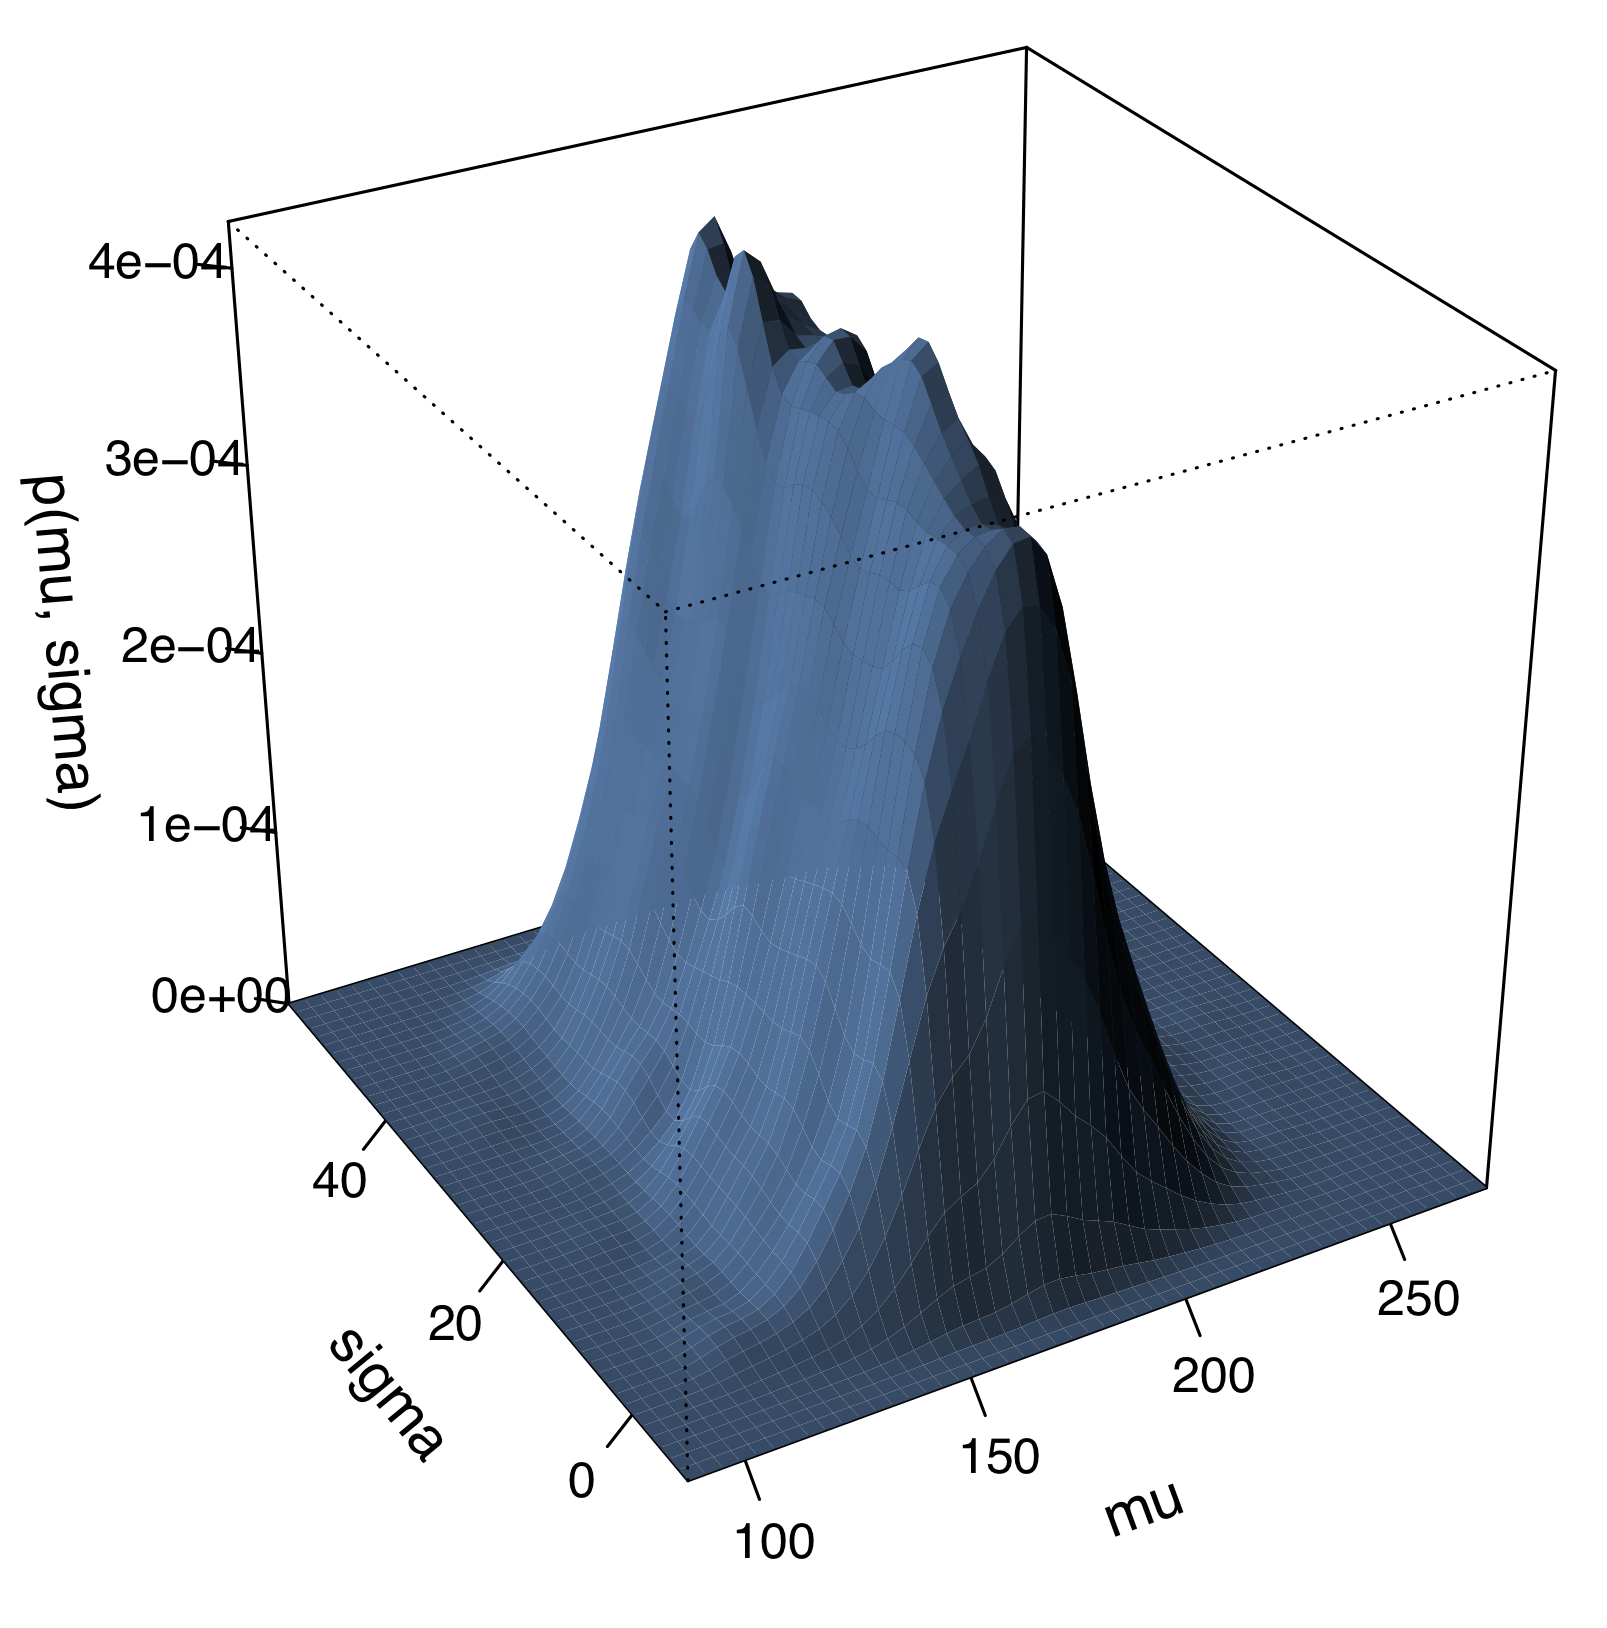
\includegraphics[width=0.75\linewidth]{figures/prior} 

}

\caption{blah blah...}\label{fig:plot-prior-2d-knitr}
\end{figure}

\hypertarget{uxe9chantillonner-uxe0-partir-du-prior}{%
\section{Échantillonner à partir du prior}\label{uxe9chantillonner-uxe0-partir-du-prior}}

\begin{Shaded}
\begin{Highlighting}[]
\NormalTok{sample\_mu \textless{}{-}}\StringTok{ }\KeywordTok{rnorm}\NormalTok{(}\DecValTok{1000}\NormalTok{, }\DecValTok{178}\NormalTok{, }\DecValTok{20}\NormalTok{)}
\NormalTok{sample\_sigma \textless{}{-}}\StringTok{ }\KeywordTok{runif}\NormalTok{(}\DecValTok{1000}\NormalTok{, }\DecValTok{0}\NormalTok{, }\DecValTok{50}\NormalTok{)}

\KeywordTok{data.frame}\NormalTok{(}\DataTypeTok{x =} \KeywordTok{rnorm}\NormalTok{(}\DecValTok{1000}\NormalTok{, sample\_mu, sample\_sigma) ) }\OperatorTok{\%\textgreater{}\%}
\StringTok{    }\KeywordTok{ggplot}\NormalTok{(}\KeywordTok{aes}\NormalTok{(x) ) }\OperatorTok{+}
\StringTok{    }\KeywordTok{geom\_histogram}\NormalTok{() }\OperatorTok{+}
\StringTok{    }\KeywordTok{xlab}\NormalTok{(}\KeywordTok{expression}\NormalTok{(y[i]) ) }\OperatorTok{+}
\StringTok{    }\KeywordTok{theme\_bw}\NormalTok{(}\DataTypeTok{base\_size =} \DecValTok{20}\NormalTok{)}
\end{Highlighting}
\end{Shaded}

\begin{figure}[!htb]

{\centering 
\includegraphics[width=0.75\linewidth]{IMSB_files/figure-latex/plot-prior-sigma-1} 

}

\caption{blah blah...}\label{fig:plot-prior-sigma}
\end{figure}

\hypertarget{fonction-de-vraisemblance}{%
\section{Fonction de vraisemblance}\label{fonction-de-vraisemblance}}

\begin{Shaded}
\begin{Highlighting}[]
\NormalTok{mu\_exemple \textless{}{-}}\StringTok{ }\FloatTok{151.23}
\NormalTok{sigma\_exemple \textless{}{-}}\StringTok{ }\FloatTok{23.42}

\NormalTok{d2}\OperatorTok{$}\NormalTok{height[}\DecValTok{34}\NormalTok{] }\CommentTok{\# one observation}
\end{Highlighting}
\end{Shaded}

\begin{verbatim}
## [1] 162.8648
\end{verbatim}

\begin{figure}[!htb]

{\centering 
\includegraphics[width=0.75\linewidth]{IMSB_files/figure-latex/likelihood-plot-1} 

}

\caption{blah blah...}\label{fig:likelihood-plot}
\end{figure}

On veut calculer la probabilité d'observer une certaine valeur de taille, sachant certaines valeurs de \(\mu\) et \(\sigma\), c'est à dire :

\[
p(x \ | \ \mu, \sigma) = \frac{1}{\sqrt{2 \pi \sigma^{2}}} \exp \bigg[-\frac{1}{2 \sigma^{2}} (\mu - x)^{2} \bigg]
\]

On peut calculer cette \emph{densité de probabilité} à l'aide des fonctions \texttt{dnorm}, \texttt{dbeta}, \texttt{dt}, \texttt{dexp}, \texttt{dgamma}, etc.

\begin{Shaded}
\begin{Highlighting}[]
\KeywordTok{dnorm}\NormalTok{(d2}\OperatorTok{$}\NormalTok{height[}\DecValTok{34}\NormalTok{], mu\_exemple, sigma\_exemple)}
\end{Highlighting}
\end{Shaded}

\begin{verbatim}
## [1] 0.01505675
\end{verbatim}

\[
p(x \ | \ \mu, \sigma) = \frac{1}{\sqrt{2 \pi \sigma^{2}}} \exp \bigg[-\frac{1}{2 \sigma^{2}} (\mu - x)^{2} \bigg]
\]

Ou à la main\ldots{}

\begin{Shaded}
\begin{Highlighting}[]
\NormalTok{normal\_likelihood \textless{}{-}}\StringTok{ }\ControlFlowTok{function}\NormalTok{ (x, mu, sigma) \{}
  
\NormalTok{  bell \textless{}{-}}\StringTok{ }\KeywordTok{exp}\NormalTok{( (}\OperatorTok{{-}}\StringTok{ }\DecValTok{1} \OperatorTok{/}\StringTok{ }\NormalTok{(}\DecValTok{2} \OperatorTok{*}\StringTok{ }\NormalTok{sigma}\OperatorTok{\^{}}\DecValTok{2}\NormalTok{) ) }\OperatorTok{*}\StringTok{ }\NormalTok{(mu }\OperatorTok{{-}}\StringTok{ }\NormalTok{x)}\OperatorTok{\^{}}\DecValTok{2}\NormalTok{ )}
\NormalTok{  norm \textless{}{-}}\StringTok{ }\KeywordTok{sqrt}\NormalTok{(}\DecValTok{2} \OperatorTok{*}\StringTok{ }\NormalTok{pi }\OperatorTok{*}\StringTok{ }\NormalTok{sigma}\OperatorTok{\^{}}\DecValTok{2}\NormalTok{)}
  
  \KeywordTok{return}\NormalTok{(bell }\OperatorTok{/}\StringTok{ }\NormalTok{norm)}
  
\NormalTok{\}}
\end{Highlighting}
\end{Shaded}

\begin{Shaded}
\begin{Highlighting}[]
\KeywordTok{normal\_likelihood}\NormalTok{(d2}\OperatorTok{$}\NormalTok{height[}\DecValTok{34}\NormalTok{], mu\_exemple, sigma\_exemple)}
\end{Highlighting}
\end{Shaded}

\begin{verbatim}
## [1] 0.01505675
\end{verbatim}

\hypertarget{distribution-postuxe9rieure}{%
\section{Distribution postérieure}\label{distribution-postuxe9rieure}}

\[
\color{purple}{p(\mu, \sigma \ | \ h)} = \frac{\prod_{i} \color{orangered}{\mathrm{Normal}(h_{i} \ | \ \mu, \sigma)}\color{steelblue}{\mathrm{Normal}(\mu \ | \ 178, 20)\mathrm{Uniform}(\sigma \ | \ 0, 50)}}
{\color{green}{\int \int \prod_{i} \mathrm{Normal}(h_{i} \ | \ \mu, \sigma)\mathrm{Normal}(\mu \ | \ 178, 20)\mathrm{Uniform}(\sigma \ | \ 0, 50) \mathrm{d} \mu \mathrm{d} \sigma}}
\]

\[
\color{purple}{p(\mu, \sigma \ | \ h)} \propto \prod_{i} \color{orangered}{\mathrm{Normal}(h_{i} \ | \ \mu, \sigma)}\color{steelblue}{\mathrm{Normal}(\mu \ | \ 178, 20)\mathrm{Uniform}(\sigma \ | \ 0, 50)}
\]

Il s'agit de la même formule vue lors des cours 1 et 2, mais cette fois en considérant qu'il existe plusieurs observations de taille (\(h_{i}\)), et deux paramètres à estimer \(\mu\) et \(\sigma\).

Pour calculer la \textbf{vraisemblance marginale} (en vert), il faut donc intégrer sur deux paramètres : \(\mu\) et \(\sigma\).

On réalise ici encore que la probabilité a posteriori est proportionnelle au produit de la vraisemblance et du prior.

\hypertarget{distribution-postuxe9rieure---grid-approximation}{%
\subsection{Distribution postérieure - grid approximation}\label{distribution-postuxe9rieure---grid-approximation}}

\begin{Shaded}
\begin{Highlighting}[]
\CommentTok{\# définit une grille de valeurs possibles pour mu et sigma}
\NormalTok{mu.list \textless{}{-}}\StringTok{ }\KeywordTok{seq}\NormalTok{(}\DataTypeTok{from =} \DecValTok{140}\NormalTok{, }\DataTypeTok{to =} \DecValTok{160}\NormalTok{, }\DataTypeTok{length.out =} \DecValTok{200}\NormalTok{)}
\NormalTok{sigma.list \textless{}{-}}\StringTok{ }\KeywordTok{seq}\NormalTok{(}\DataTypeTok{from =} \DecValTok{4}\NormalTok{, }\DataTypeTok{to =} \DecValTok{9}\NormalTok{, }\DataTypeTok{length.out =} \DecValTok{200}\NormalTok{)}

\CommentTok{\# étend la grille en deux dimensions (chaque combinaison de mu et sigma)}
\NormalTok{post \textless{}{-}}\StringTok{ }\KeywordTok{expand.grid}\NormalTok{(}\DataTypeTok{mu =}\NormalTok{ mu.list, }\DataTypeTok{sigma =}\NormalTok{ sigma.list)}

\CommentTok{\# calcul de la log{-}vraisemblance (pour chaque couple de mu et sigma)}
\NormalTok{post}\OperatorTok{$}\NormalTok{LL \textless{}{-}}
\StringTok{  }\KeywordTok{sapply}\NormalTok{(}
    \DecValTok{1}\OperatorTok{:}\KeywordTok{nrow}\NormalTok{(post),}
    \ControlFlowTok{function}\NormalTok{(i) }\KeywordTok{sum}\NormalTok{(}\KeywordTok{dnorm}\NormalTok{(}
\NormalTok{      d2}\OperatorTok{$}\NormalTok{height,}
      \DataTypeTok{mean =}\NormalTok{ post}\OperatorTok{$}\NormalTok{mu[i],}
      \DataTypeTok{sd =}\NormalTok{ post}\OperatorTok{$}\NormalTok{sigma[i],}
      \DataTypeTok{log =} \OtherTok{TRUE}\NormalTok{)}
\NormalTok{      )}
\NormalTok{    )}

\CommentTok{\# calcul de la probabilité a posteriori (non normalisée)}
\NormalTok{post}\OperatorTok{$}\NormalTok{prod \textless{}{-}}
\StringTok{  }\NormalTok{post}\OperatorTok{$}\NormalTok{LL }\OperatorTok{+}
\StringTok{  }\KeywordTok{dnorm}\NormalTok{(post}\OperatorTok{$}\NormalTok{mu, }\DecValTok{178}\NormalTok{, }\DecValTok{20}\NormalTok{, }\DataTypeTok{log =} \OtherTok{TRUE}\NormalTok{) }\OperatorTok{+}
\StringTok{  }\KeywordTok{dunif}\NormalTok{(post}\OperatorTok{$}\NormalTok{sigma, }\DecValTok{0}\NormalTok{, }\DecValTok{50}\NormalTok{, }\DataTypeTok{log =} \OtherTok{TRUE}\NormalTok{)}

\CommentTok{\# on "annule" le log en avec exp() et on standardise par la valeur maximale}
\NormalTok{post}\OperatorTok{$}\NormalTok{prob \textless{}{-}}\StringTok{ }\KeywordTok{exp}\NormalTok{(post}\OperatorTok{$}\NormalTok{prod }\OperatorTok{{-}}\StringTok{ }\KeywordTok{max}\NormalTok{(post}\OperatorTok{$}\NormalTok{prod) )}
\end{Highlighting}
\end{Shaded}

\begin{Shaded}
\begin{Highlighting}[]
\NormalTok{sample.rows \textless{}{-}}\StringTok{ }\KeywordTok{sample}\NormalTok{(}\DecValTok{1}\OperatorTok{:}\KeywordTok{nrow}\NormalTok{(post), }\DataTypeTok{size =} \FloatTok{1e4}\NormalTok{, }\DataTypeTok{replace =} \OtherTok{TRUE}\NormalTok{, }\DataTypeTok{prob =}\NormalTok{ post}\OperatorTok{$}\NormalTok{prob)}
\end{Highlighting}
\end{Shaded}

\begin{figure}[!htb]

{\centering 
\includegraphics[width=0.75\linewidth]{IMSB_files/figure-latex/plotting-samples-1} 

}

\caption{blah blah...}\label{fig:plotting-samples}
\end{figure}

\hypertarget{distribution-postuxe9rieure---distributions-marginales}{%
\subsection{Distribution postérieure - distributions marginales}\label{distribution-postuxe9rieure---distributions-marginales}}

\begin{Shaded}
\begin{Highlighting}[]
\NormalTok{BEST}\OperatorTok{::}\KeywordTok{plotPost}\NormalTok{(}
\NormalTok{  sample.mu, }\DataTypeTok{breaks =} \DecValTok{40}\NormalTok{, }\DataTypeTok{xlab =} \KeywordTok{expression}\NormalTok{(mu)}
\NormalTok{  )}
\end{Highlighting}
\end{Shaded}

\begin{figure}[!htb]

{\centering 
\includegraphics[width=0.75\linewidth]{IMSB_files/figure-latex/unnamed-chunk-20-1} 

}

\caption{blah blah...}\label{fig:unnamed-chunk-20}
\end{figure}

\begin{Shaded}
\begin{Highlighting}[]
\NormalTok{BEST}\OperatorTok{::}\KeywordTok{plotPost}\NormalTok{(}
\NormalTok{  sample.sigma, }\DataTypeTok{breaks =} \DecValTok{40}\NormalTok{, }\DataTypeTok{xlab =} \KeywordTok{expression}\NormalTok{(sigma)}
\NormalTok{  )}
\end{Highlighting}
\end{Shaded}

\begin{figure}[!htb]

{\centering 
\includegraphics[width=0.75\linewidth]{IMSB_files/figure-latex/unnamed-chunk-21-1} 

}

\caption{blah blah...}\label{fig:unnamed-chunk-21}
\end{figure}

\hypertarget{introduction-uxe0-brms}{%
\section{Introduction à brms}\label{introduction-uxe0-brms}}

Under the hood : \texttt{Stan} est un langage de programmation probabiliste écrit en \texttt{C++}, et qui implémente plusieurs algorithmes de MCMC: HMC, NUTS, L-BFGS\ldots{}

\begin{Shaded}
\begin{Highlighting}[]
\NormalTok{data \{}
\NormalTok{  int}\OperatorTok{\textless{}}\NormalTok{lower=}\DecValTok{0}\OperatorTok{\textgreater{}}\StringTok{ }\NormalTok{J; }\OperatorTok{/}\ErrorTok{/}\StringTok{ }\NormalTok{number of schools }
\NormalTok{  real y[J]; }\OperatorTok{/}\ErrorTok{/}\StringTok{ }\NormalTok{estimated treatment effects}
\NormalTok{  real}\OperatorTok{\textless{}}\NormalTok{lower=}\DecValTok{0}\OperatorTok{\textgreater{}}\StringTok{ }\NormalTok{sigma[J]; }\OperatorTok{/}\ErrorTok{/}\StringTok{ }\NormalTok{s.e. of effect estimates }
\NormalTok{\}}

\NormalTok{parameters \{}
\NormalTok{  real mu; }
\NormalTok{  real}\OperatorTok{\textless{}}\NormalTok{lower=}\DecValTok{0}\OperatorTok{\textgreater{}}\StringTok{ }\NormalTok{tau;}
\NormalTok{  real eta[J];}
\NormalTok{\}}

\NormalTok{transformed parameters \{}
\NormalTok{  real theta[J];}
  \ControlFlowTok{for}\NormalTok{ (j }\ControlFlowTok{in} \DecValTok{1}\OperatorTok{:}\NormalTok{J)}
\NormalTok{    theta[j] =}\StringTok{ }\NormalTok{mu }\OperatorTok{+}\StringTok{ }\NormalTok{tau }\OperatorTok{*}\StringTok{ }\NormalTok{eta[j];}
\NormalTok{\}}

\NormalTok{model \{}
\NormalTok{  target }\OperatorTok{+}\ErrorTok{=}\StringTok{ }\KeywordTok{normal\_lpdf}\NormalTok{(eta }\OperatorTok{|}\StringTok{ }\DecValTok{0}\NormalTok{, }\DecValTok{1}\NormalTok{);}
\NormalTok{  target }\OperatorTok{+}\ErrorTok{=}\StringTok{ }\KeywordTok{normal\_lpdf}\NormalTok{(y }\OperatorTok{|}\StringTok{ }\NormalTok{theta, sigma);}
\NormalTok{\}}
\end{Highlighting}
\end{Shaded}

Le package \texttt{brms} (\href{https://www.jstatsoft.org/article/view/v080i01}{Bürkner, 2017}) permet de fitter des modèles multi-niveaux (ou pas) linéaires (ou pas) bayésiens en \texttt{Stan} mais en utilisant la syntaxe de \texttt{lme4}.

Par exemple, le modèle suivant :

\[
\begin{aligned}
y_{i} &\sim \mathrm{Normal}(\mu_{i}, \sigma) \\
\mu_{i} &= \alpha + \alpha_{subject[i]} + \alpha_{item[i]} + \beta x_{i} \\
\end{aligned}
\]

se spécifie avec \texttt{brms} (comme avec \texttt{lme4}) de la manière suivante :

\begin{Shaded}
\begin{Highlighting}[]
\KeywordTok{brm}\NormalTok{(y }\OperatorTok{\textasciitilde{}}\StringTok{ }\NormalTok{x }\OperatorTok{+}\StringTok{ }\NormalTok{(}\DecValTok{1} \OperatorTok{|}\StringTok{ }\NormalTok{subject) }\OperatorTok{+}\StringTok{ }\NormalTok{(}\DecValTok{1} \OperatorTok{|}\StringTok{ }\NormalTok{item), }\DataTypeTok{data =}\NormalTok{ d, }\DataTypeTok{family =} \KeywordTok{gaussian}\NormalTok{() )}
\end{Highlighting}
\end{Shaded}

\hypertarget{rappels-de-syntaxe}{%
\subsection{Rappels de syntaxe}\label{rappels-de-syntaxe}}

Le package \texttt{brms} utilise la même syntaxe que les fonctions de base R (comme \texttt{lm}) ou que le package \texttt{lme4}.

\begin{Shaded}
\begin{Highlighting}[]
\NormalTok{Reaction }\OperatorTok{\textasciitilde{}}\StringTok{ }\NormalTok{Days }\OperatorTok{+}\StringTok{ }\NormalTok{(}\DecValTok{1} \OperatorTok{+}\StringTok{ }\NormalTok{Days }\OperatorTok{|}\StringTok{ }\NormalTok{Subject)}
\end{Highlighting}
\end{Shaded}

La partie gauche représente notre variable dépendante (ou \emph{outcome}, i.e., ce qu'on essaye de prédire). Le package \texttt{brms} permet également de fitter des modèles multivariés (plusieurs outcomes) en les combinant avec \texttt{mvbind()}:

\begin{Shaded}
\begin{Highlighting}[]
\KeywordTok{mvbind}\NormalTok{(Reaction, Memory) }\OperatorTok{\textasciitilde{}}\StringTok{ }\NormalTok{Days }\OperatorTok{+}\StringTok{ }\NormalTok{(}\DecValTok{1} \OperatorTok{+}\StringTok{ }\NormalTok{Days }\OperatorTok{|}\StringTok{ }\NormalTok{Subject)}
\end{Highlighting}
\end{Shaded}

La partie droite permet de définir les prédicteurs. L'intercept est généralement implicite, de sorte que les deux écritures ci-dessous sont équivalentes.

\begin{Shaded}
\begin{Highlighting}[]
\KeywordTok{mvbind}\NormalTok{(Reaction, Memory) }\OperatorTok{\textasciitilde{}}\StringTok{ }\NormalTok{Days }\OperatorTok{+}\StringTok{ }\NormalTok{(}\DecValTok{1} \OperatorTok{+}\StringTok{ }\NormalTok{Days }\OperatorTok{|}\StringTok{ }\NormalTok{Subject)}
\KeywordTok{mvbind}\NormalTok{(Reaction, Memory) }\OperatorTok{\textasciitilde{}}\StringTok{ }\DecValTok{1} \OperatorTok{+}\StringTok{ }\NormalTok{Days }\OperatorTok{+}\StringTok{ }\NormalTok{(}\DecValTok{1} \OperatorTok{+}\StringTok{ }\NormalTok{Days }\OperatorTok{|}\StringTok{ }\NormalTok{Subject)}
\end{Highlighting}
\end{Shaded}

Si l'on veut fitter un modèle sans intercept (why not), il faut le spécifier explicitement comme ci-dessous.

\begin{Shaded}
\begin{Highlighting}[]
\KeywordTok{mvbind}\NormalTok{(Reaction, Memory) }\OperatorTok{\textasciitilde{}}\StringTok{ }\DecValTok{0} \OperatorTok{+}\StringTok{ }\NormalTok{Days }\OperatorTok{+}\StringTok{ }\NormalTok{(}\DecValTok{1} \OperatorTok{+}\StringTok{ }\NormalTok{Days }\OperatorTok{|}\StringTok{ }\NormalTok{Subject)}
\end{Highlighting}
\end{Shaded}

Par défaut \texttt{brms} postule une vraisemblance gaussienne. Ce postulat peut être changé facilement en spécifiant la vraisemblance souhaitée via l'argument \texttt{family}.

\begin{Shaded}
\begin{Highlighting}[]
\KeywordTok{brm}\NormalTok{(Reaction }\OperatorTok{\textasciitilde{}}\StringTok{ }\DecValTok{1} \OperatorTok{+}\StringTok{ }\NormalTok{Days }\OperatorTok{+}\StringTok{ }\NormalTok{(}\DecValTok{1} \OperatorTok{+}\StringTok{ }\NormalTok{Days }\OperatorTok{|}\StringTok{ }\NormalTok{Subject), }\DataTypeTok{family =} \KeywordTok{lognormal}\NormalTok{() )}
\end{Highlighting}
\end{Shaded}

Lisez la documentation (c'est très enthousiasmant à lire) accessible via \texttt{?brm}.

\hypertarget{quelques-fonctions-utiles}{%
\subsection{Quelques fonctions utiles}\label{quelques-fonctions-utiles}}

\begin{Shaded}
\begin{Highlighting}[]
\CommentTok{\# Generate the Stan code:}
\KeywordTok{make\_stancode}\NormalTok{(formula, ...)}
\KeywordTok{stancode}\NormalTok{(fit)}

\CommentTok{\# Generate the data passed to Stan:}
\KeywordTok{make\_standata}\NormalTok{(formula, ...)}
\KeywordTok{standata}\NormalTok{(fit)}

\CommentTok{\# Handle priors:}
\KeywordTok{get\_prior}\NormalTok{(formula, ...)}
\KeywordTok{set\_prior}\NormalTok{(prior, ...)}

\CommentTok{\# Generate expected values and predictions:}
\KeywordTok{fitted}\NormalTok{(fit, ...)}
\KeywordTok{predict}\NormalTok{(fit, ...)}
\KeywordTok{marginal\_effects}\NormalTok{(fit, ...)}

\CommentTok{\# Model comparison:}
\KeywordTok{loo}\NormalTok{(fit1, fit2, ...)}
\KeywordTok{bayes\_factor}\NormalTok{(fit1, fit2, ...)}
\KeywordTok{model\_weights}\NormalTok{(fit1, fit2, ...)}

\CommentTok{\# Hypothesis testing:}
\KeywordTok{hypothesis}\NormalTok{(fit, hypothesis, ...)}
\end{Highlighting}
\end{Shaded}

\hypertarget{un-premier-exemple}{%
\subsection{Un premier exemple}\label{un-premier-exemple}}

\begin{Shaded}
\begin{Highlighting}[]
\KeywordTok{library}\NormalTok{(brms)}
\NormalTok{mod1 \textless{}{-}}\StringTok{ }\KeywordTok{brm}\NormalTok{(height }\OperatorTok{\textasciitilde{}}\StringTok{ }\DecValTok{1}\NormalTok{, }\DataTypeTok{data =}\NormalTok{ d2)}
\end{Highlighting}
\end{Shaded}

\begin{Shaded}
\begin{Highlighting}[]
\KeywordTok{rbind}\NormalTok{(}\KeywordTok{summary}\NormalTok{(mod1)}\OperatorTok{$}\NormalTok{fixed, }\KeywordTok{summary}\NormalTok{(mod1)}\OperatorTok{$}\NormalTok{spec\_pars )}
\end{Highlighting}
\end{Shaded}

\begin{verbatim}
##             Estimate Est.Error   l-95% CI   u-95% CI     Rhat Bulk_ESS Tail_ESS
## Intercept 154.592895 0.4100465 153.797098 155.385549 1.001129     2872     2195
## sigma       7.754854 0.2886444   7.223486   8.342585 1.000546     4002     2612
\end{verbatim}

Ces données représentent les distributions marginales de chaque paramètre. En d'autres termes, la \emph{probabilité} de chaque valeur de \(\mu\), après avoir \emph{moyenné} sur toutes les valeurs possible de \(\sigma\), est décrite par une distribution gaussienne avec une moyenne de \(154.61\) et un écart type de \(0.41\). L'intervalle de crédibilité (\(\neq\) intervalle de confiance) nous indique les 95\% valeurs de \(\mu\) ou \(\sigma\) les plus probables (sachant les données et les priors).

\hypertarget{en-utilisant-notre-prior}{%
\subsection{En utilisant notre prior}\label{en-utilisant-notre-prior}}

Par défaut \texttt{brms} utilise un prior très peu informatif centré sur la valeur moyenne de la variable mesurée. On peut donc affiner l'estimation réalisée par ce modèle en utilisant nos connaissances sur la distribution habituelle des tailles chez les humains.

La fonction \texttt{get\_prior()} permet de visualiser une liste des priors par défaut ainsi que de tous les prios qu'on peut spécifier, sachant une certaine formule (i.e., une manière d'écrire notre modèle) et un jeu de données.

\begin{Shaded}
\begin{Highlighting}[]
\KeywordTok{get\_prior}\NormalTok{(height }\OperatorTok{\textasciitilde{}}\StringTok{ }\DecValTok{1}\NormalTok{, }\DataTypeTok{data =}\NormalTok{ d2)}
\end{Highlighting}
\end{Shaded}

\begin{verbatim}
##                   prior     class coef group resp dpar nlpar bound
## 1 student_t(3, 154, 10) Intercept                                 
## 2   student_t(3, 0, 10)     sigma
\end{verbatim}

\ldots{}

\begin{Shaded}
\begin{Highlighting}[]
\NormalTok{priors \textless{}{-}}\StringTok{ }\KeywordTok{c}\NormalTok{(}
  \KeywordTok{prior}\NormalTok{(}\KeywordTok{normal}\NormalTok{(}\DecValTok{178}\NormalTok{, }\DecValTok{20}\NormalTok{), }\DataTypeTok{class =}\NormalTok{ Intercept),}
  \KeywordTok{prior}\NormalTok{(}\KeywordTok{exponential}\NormalTok{(}\FloatTok{0.01}\NormalTok{), }\DataTypeTok{class =}\NormalTok{ sigma)}
\NormalTok{  )}

\NormalTok{mod2 \textless{}{-}}\StringTok{ }\KeywordTok{brm}\NormalTok{(}
\NormalTok{  height }\OperatorTok{\textasciitilde{}}\StringTok{ }\DecValTok{1}\NormalTok{,}
  \DataTypeTok{prior =}\NormalTok{ priors,}
  \DataTypeTok{family =} \KeywordTok{gaussian}\NormalTok{(),}
  \DataTypeTok{data =}\NormalTok{ d2}
\NormalTok{  )}
\end{Highlighting}
\end{Shaded}

\begin{figure}[!htb]

{\centering 
\includegraphics[width=0.75\linewidth]{IMSB_files/figure-latex/prior-mod2-1} 

}

\caption{blah blah...}\label{fig:prior-mod2}
\end{figure}

\ldots{}

\begin{Shaded}
\begin{Highlighting}[]
\KeywordTok{summary}\NormalTok{(mod2)}
\end{Highlighting}
\end{Shaded}

\begin{verbatim}
##  Family: gaussian 
##   Links: mu = identity; sigma = identity 
## Formula: height ~ 1 
##    Data: d2 (Number of observations: 352) 
## Samples: 4 chains, each with iter = 2000; warmup = 1000; thin = 1;
##          total post-warmup samples = 4000
## 
## Population-Level Effects: 
##           Estimate Est.Error l-95% CI u-95% CI Rhat Bulk_ESS Tail_ESS
## Intercept   154.61      0.42   153.79   155.42 1.00     3007     2492
## 
## Family Specific Parameters: 
##       Estimate Est.Error l-95% CI u-95% CI Rhat Bulk_ESS Tail_ESS
## sigma     7.76      0.30     7.19     8.39 1.00     2900     1979
## 
## Samples were drawn using sampling(NUTS). For each parameter, Bulk_ESS
## and Tail_ESS are effective sample size measures, and Rhat is the potential
## scale reduction factor on split chains (at convergence, Rhat = 1).
\end{verbatim}

\hypertarget{en-utilisant-un-prior-plus-informatif}{%
\subsection{En utilisant un prior plus informatif}\label{en-utilisant-un-prior-plus-informatif}}

\begin{Shaded}
\begin{Highlighting}[]
\NormalTok{priors \textless{}{-}}\StringTok{ }\KeywordTok{c}\NormalTok{(}
  \KeywordTok{prior}\NormalTok{(}\KeywordTok{normal}\NormalTok{(}\DecValTok{178}\NormalTok{, }\FloatTok{0.1}\NormalTok{), }\DataTypeTok{class =}\NormalTok{ Intercept),}
  \KeywordTok{prior}\NormalTok{(}\KeywordTok{exponential}\NormalTok{(}\FloatTok{0.01}\NormalTok{), }\DataTypeTok{class =}\NormalTok{ sigma)}
\NormalTok{  )}

\NormalTok{mod3 \textless{}{-}}\StringTok{ }\KeywordTok{brm}\NormalTok{(}
\NormalTok{  height }\OperatorTok{\textasciitilde{}}\StringTok{ }\DecValTok{1}\NormalTok{,}
  \DataTypeTok{prior =}\NormalTok{ priors,}
  \DataTypeTok{family =} \KeywordTok{gaussian}\NormalTok{(),}
  \DataTypeTok{data =}\NormalTok{ d2}
\NormalTok{  )}
\end{Highlighting}
\end{Shaded}

\begin{figure}[!htb]

{\centering 
\includegraphics[width=0.75\linewidth]{IMSB_files/figure-latex/prior-mod3-1} 

}

\caption{blah blah...}\label{fig:prior-mod3}
\end{figure}

\ldots{}

\begin{Shaded}
\begin{Highlighting}[]
\KeywordTok{summary}\NormalTok{(mod3)}
\end{Highlighting}
\end{Shaded}

\begin{verbatim}
##  Family: gaussian 
##   Links: mu = identity; sigma = identity 
## Formula: height ~ 1 
##    Data: d2 (Number of observations: 352) 
## Samples: 4 chains, each with iter = 2000; warmup = 1000; thin = 1;
##          total post-warmup samples = 4000
## 
## Population-Level Effects: 
##           Estimate Est.Error l-95% CI u-95% CI Rhat Bulk_ESS Tail_ESS
## Intercept   177.86      0.10   177.67   178.06 1.00     3030     2653
## 
## Family Specific Parameters: 
##       Estimate Est.Error l-95% CI u-95% CI Rhat Bulk_ESS Tail_ESS
## sigma    24.61      0.94    22.84    26.51 1.00     2852     2513
## 
## Samples were drawn using sampling(NUTS). For each parameter, Bulk_ESS
## and Tail_ESS are effective sample size measures, and Rhat is the potential
## scale reduction factor on split chains (at convergence, Rhat = 1).
\end{verbatim}

On remarque que la valeur estimée pour \(\mu\) n'a presque pas ``bougée'' du prior\ldots mais on remarque également que la valeur estimée pour \(\sigma\) a largement augmentée. Nous avons dit au modèle que nous étions assez certain de notre valeur de \(\mu\), le modèle s'est ensuite ``adapté'', ce qui explique la valeur de \(\sigma\)\ldots{}

\hypertarget{pruxe9cision-du-prior-heuristique}{%
\subsection{Précision du prior (heuristique)}\label{pruxe9cision-du-prior-heuristique}}

Le prior peut généralement être considéré comme un posterior obtenu sur des données antérieures.

On sait que le \(\sigma\) d'un posterior gaussien nous est donné par la formule:

\[\sigma_{post} = 1 / \sqrt{n}\]

Qui implique une \emph{quantité de données} \(n = 1 / \sigma^2_{post}\). Notre prior avait un \(\sigma = 0.1\), ce qui donne \(n = 1 / 0.1^2 = 100\).

Donc, on peut considérer que le prior \(\mu \sim \mathrm{Normal}(178, 0.1)\) est équivalent au cas dans lequel nous aurions observé \(100\) tailles de moyenne \(178\).

\hypertarget{ruxe9cupuxe9rer-et-visualiser-les-uxe9chantillons-de-la-distribution-postuxe9rieure}{%
\subsection{Récupérer et visualiser les échantillons de la distribution postérieure}\label{ruxe9cupuxe9rer-et-visualiser-les-uxe9chantillons-de-la-distribution-postuxe9rieure}}

\begin{Shaded}
\begin{Highlighting}[]
\NormalTok{post \textless{}{-}}\StringTok{ }\KeywordTok{posterior\_samples}\NormalTok{(mod2) }\OperatorTok{\%\textgreater{}\%}
\StringTok{    }\KeywordTok{mutate}\NormalTok{(}\DataTypeTok{density =} \KeywordTok{get\_density}\NormalTok{(b\_Intercept, sigma, }\DataTypeTok{n =} \FloatTok{1e2}\NormalTok{) )}

\KeywordTok{ggplot}\NormalTok{(post, }\KeywordTok{aes}\NormalTok{(}\DataTypeTok{x =}\NormalTok{ b\_Intercept, }\DataTypeTok{y =}\NormalTok{ sigma, }\DataTypeTok{color =}\NormalTok{ density) ) }\OperatorTok{+}
\StringTok{    }\KeywordTok{geom\_point}\NormalTok{(}\DataTypeTok{size =} \DecValTok{2}\NormalTok{, }\DataTypeTok{alpha =} \FloatTok{0.5}\NormalTok{, }\DataTypeTok{show.legend =} \OtherTok{FALSE}\NormalTok{) }\OperatorTok{+}
\StringTok{    }\KeywordTok{theme\_bw}\NormalTok{(}\DataTypeTok{base\_size =} \DecValTok{20}\NormalTok{) }\OperatorTok{+}
\StringTok{    }\KeywordTok{labs}\NormalTok{(}\DataTypeTok{x =} \KeywordTok{expression}\NormalTok{(mu), }\DataTypeTok{y =} \KeywordTok{expression}\NormalTok{(sigma) ) }\OperatorTok{+}
\StringTok{    }\NormalTok{viridis}\OperatorTok{::}\KeywordTok{scale\_color\_viridis}\NormalTok{()}
\end{Highlighting}
\end{Shaded}

\begin{figure}[!htb]

{\centering 
\includegraphics[width=0.75\linewidth]{IMSB_files/figure-latex/samples-plot-1} 

}

\caption{blah blah...}\label{fig:samples-plot}
\end{figure}

\hypertarget{ruxe9cupuxe9rer-les-uxe9chantillons-de-la-distribution-postuxe9rieure}{%
\subsection{Récupérer les échantillons de la distribution postérieure}\label{ruxe9cupuxe9rer-les-uxe9chantillons-de-la-distribution-postuxe9rieure}}

\begin{Shaded}
\begin{Highlighting}[]
\CommentTok{\# gets the first 6 samples}
\KeywordTok{head}\NormalTok{(post)}
\end{Highlighting}
\end{Shaded}

\begin{verbatim}
##   b_Intercept    sigma      lp__   density
## 1    154.5939 8.062182 -1227.204 0.6520986
## 2    154.5531 8.074903 -1227.256 0.6514711
## 3    154.3450 7.449061 -1227.392 0.6161563
## 4    154.4178 7.911728 -1226.906 0.9177760
## 5    154.4087 7.620968 -1226.847 0.9938276
## 6    154.9646 7.641722 -1227.086 1.0039033
\end{verbatim}

\begin{Shaded}
\begin{Highlighting}[]
\CommentTok{\# gets the median and the 95\% credible interval}
\KeywordTok{t}\NormalTok{(}\KeywordTok{sapply}\NormalTok{(post[, }\DecValTok{1}\OperatorTok{:}\DecValTok{2}\NormalTok{], quantile, }\DataTypeTok{probs =} \KeywordTok{c}\NormalTok{(}\FloatTok{0.025}\NormalTok{, }\FloatTok{0.5}\NormalTok{, }\FloatTok{0.975}\NormalTok{) ) )}
\end{Highlighting}
\end{Shaded}

\begin{verbatim}
##                  2.5%        50%      97.5%
## b_Intercept 153.79095 154.622493 155.420107
## sigma         7.19174   7.754505   8.385922
\end{verbatim}

\hypertarget{visualiser-la-distribution-postuxe9rieure}{%
\subsection{Visualiser la distribution postérieure}\label{visualiser-la-distribution-postuxe9rieure}}

\begin{Shaded}
\begin{Highlighting}[]
\NormalTok{H.scv \textless{}{-}}\StringTok{ }\KeywordTok{Hscv}\NormalTok{(post[, }\DecValTok{1}\OperatorTok{:}\DecValTok{2}\NormalTok{])}
\NormalTok{fhat\_post \textless{}{-}}\StringTok{ }\KeywordTok{kde}\NormalTok{(}\DataTypeTok{x =}\NormalTok{ post[, }\DecValTok{1}\OperatorTok{:}\DecValTok{2}\NormalTok{], }\DataTypeTok{H =}\NormalTok{ H.scv, }\DataTypeTok{compute.cont =} \OtherTok{TRUE}\NormalTok{)}

\KeywordTok{plot}\NormalTok{(fhat\_post, }\DataTypeTok{display =} \StringTok{"persp"}\NormalTok{, }\DataTypeTok{col =} \StringTok{"purple"}\NormalTok{, }\DataTypeTok{border =} \OtherTok{NA}\NormalTok{,}
  \DataTypeTok{xlab =} \StringTok{"}\CharTok{\textbackslash{}n}\StringTok{mu"}\NormalTok{, }\DataTypeTok{ylab =} \StringTok{"}\CharTok{\textbackslash{}n}\StringTok{sigma"}\NormalTok{, }\DataTypeTok{zlab =} \StringTok{"}\CharTok{\textbackslash{}n}\StringTok{p(mu, sigma)"}\NormalTok{,}
  \DataTypeTok{shade =} \FloatTok{0.8}\NormalTok{, }\DataTypeTok{phi =} \DecValTok{30}\NormalTok{, }\DataTypeTok{ticktype =} \StringTok{"detailed"}\NormalTok{,}
  \DataTypeTok{cex.lab =} \FloatTok{1.2}\NormalTok{, }\DataTypeTok{family =} \StringTok{"Helvetica"}\NormalTok{)}
\end{Highlighting}
\end{Shaded}

\begin{Shaded}
\begin{Highlighting}[]
\NormalTok{knitr}\OperatorTok{::}\KeywordTok{include\_graphics}\NormalTok{(}\StringTok{"figures/posterior.png"}\NormalTok{)}
\end{Highlighting}
\end{Shaded}

\begin{figure}[!htb]

{\centering 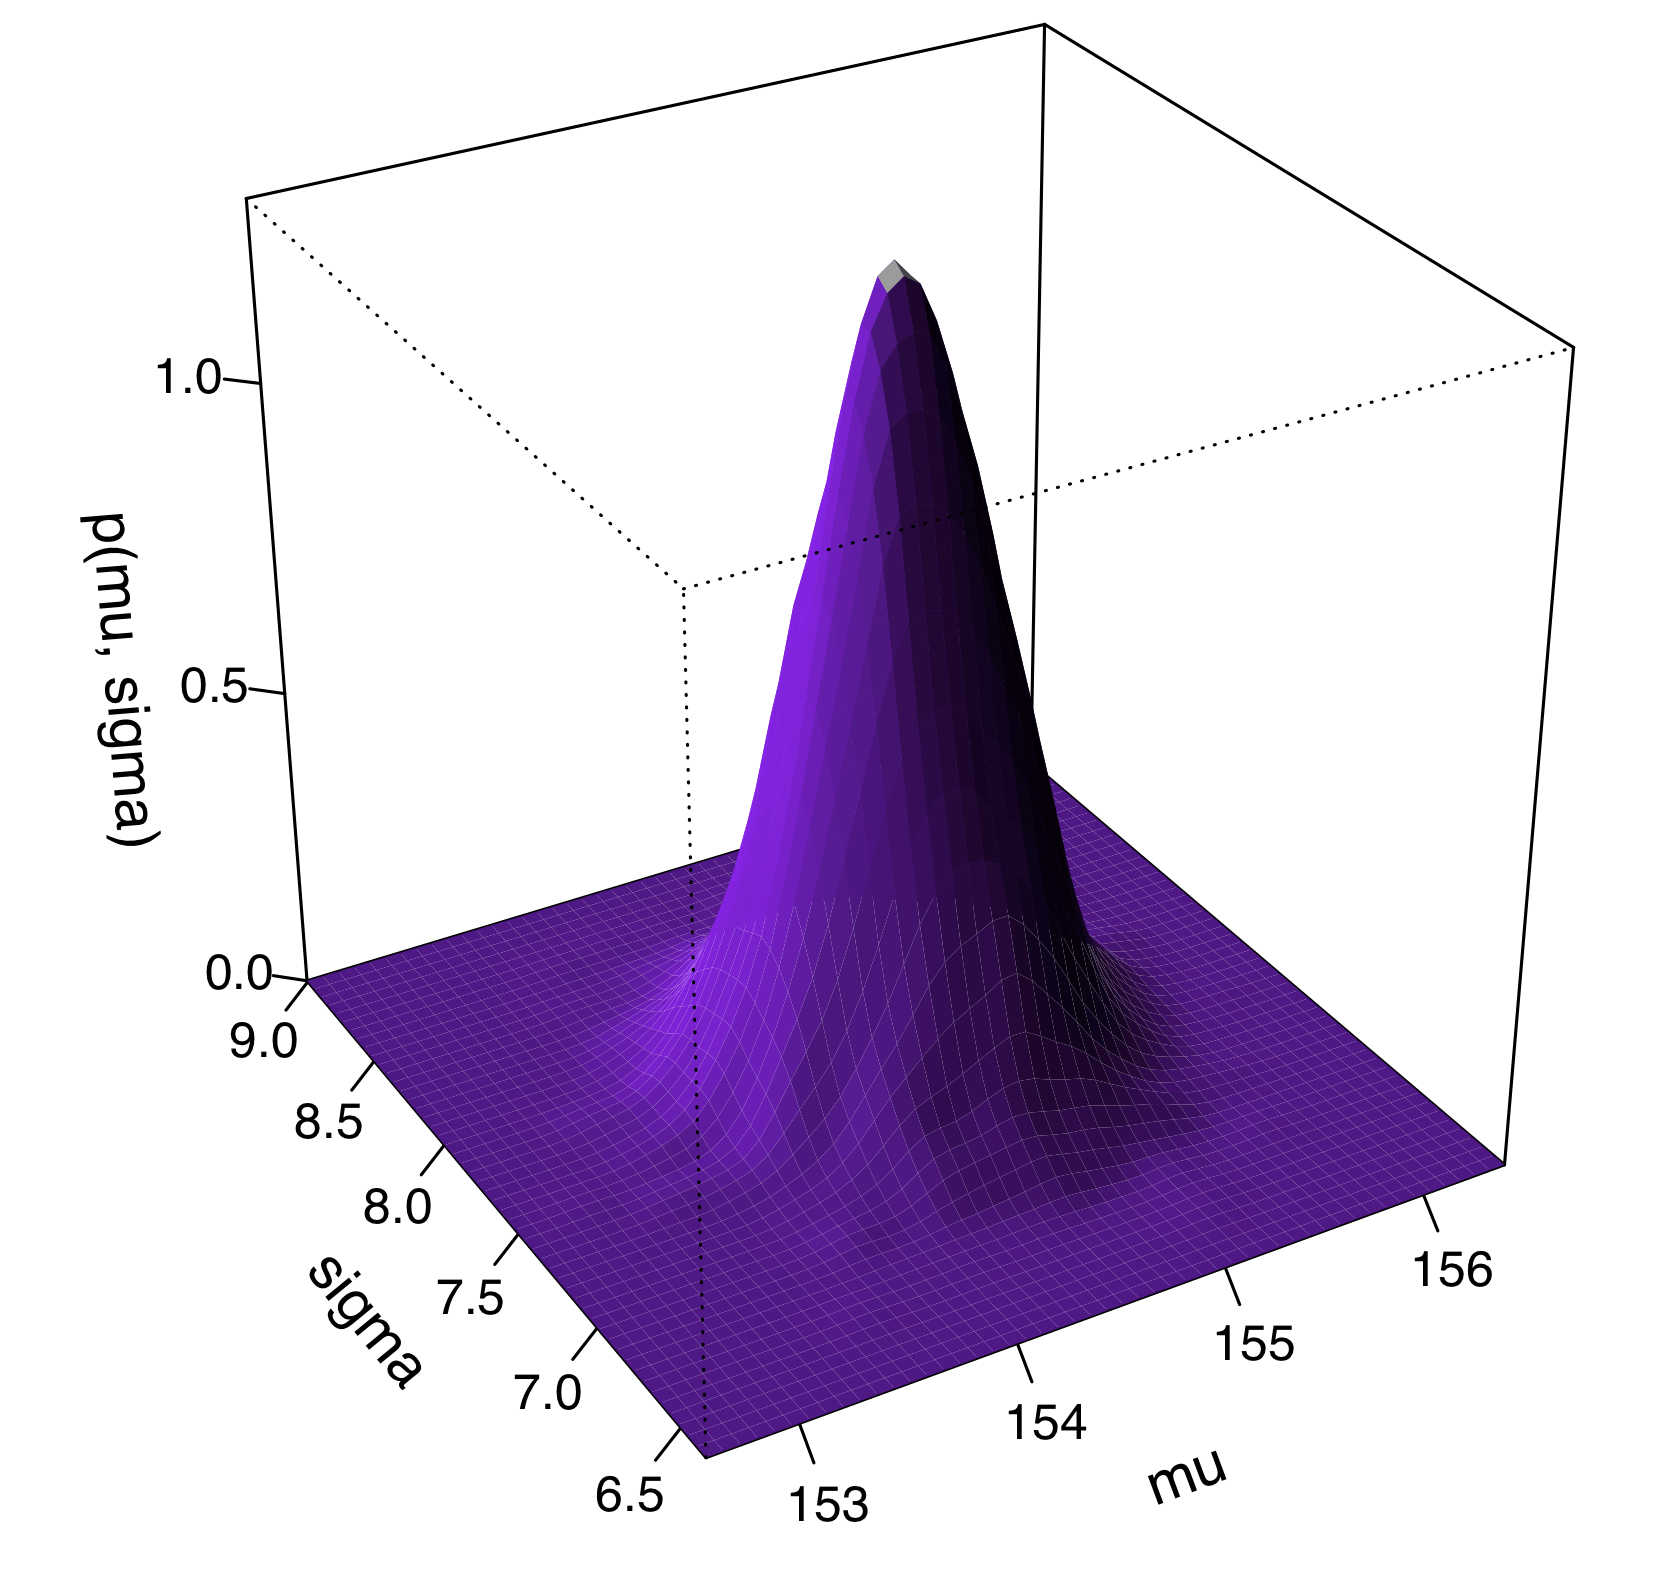
\includegraphics[width=0.75\linewidth]{figures/posterior} 

}

\caption{blah blah...}\label{fig:unnamed-chunk-31}
\end{figure}

\hypertarget{visualiser-la-distribution-postuxe9rieure-1}{%
\subsection{Visualiser la distribution postérieure}\label{visualiser-la-distribution-postuxe9rieure-1}}

\begin{figure}[!htb]

{\centering 
\includegraphics[width=0.75\linewidth]{IMSB_files/figure-latex/plot-samples-1} 

}

\caption{blah blah...}\label{fig:plot-samples}
\end{figure}

\hypertarget{ajouter-un-pruxe9dicteur}{%
\subsection{Ajouter un prédicteur}\label{ajouter-un-pruxe9dicteur}}

Comment est-ce que la taille co-varie avec le poids ?

\begin{Shaded}
\begin{Highlighting}[]
\NormalTok{d2 }\OperatorTok{\%\textgreater{}\%}
\StringTok{  }\KeywordTok{ggplot}\NormalTok{(}\KeywordTok{aes}\NormalTok{(}\DataTypeTok{x =}\NormalTok{ weight, }\DataTypeTok{y =}\NormalTok{ height) ) }\OperatorTok{+}
\StringTok{  }\KeywordTok{geom\_point}\NormalTok{(}\DataTypeTok{colour =} \StringTok{"white"}\NormalTok{, }\DataTypeTok{fill =} \StringTok{"black"}\NormalTok{, }\DataTypeTok{pch =} \DecValTok{21}\NormalTok{, }\DataTypeTok{size =} \DecValTok{3}\NormalTok{, }\DataTypeTok{alpha =} \FloatTok{0.8}\NormalTok{) }\OperatorTok{+}
\StringTok{  }\KeywordTok{theme\_bw}\NormalTok{(}\DataTypeTok{base\_size =} \DecValTok{20}\NormalTok{)}
\end{Highlighting}
\end{Shaded}

\begin{figure}[!htb]

{\centering 
\includegraphics[width=0.75\linewidth]{IMSB_files/figure-latex/height-weight-plot-1} 

}

\caption{blah blah...}\label{fig:height-weight-plot}
\end{figure}

\hypertarget{ruxe9gression-linuxe9aire-uxe0-un-pruxe9dicteur-continu}{%
\section{Régression linéaire à un prédicteur continu}\label{ruxe9gression-linuxe9aire-uxe0-un-pruxe9dicteur-continu}}

\[
\begin{aligned}
h_{i} &\sim \mathrm{Normal}(\mu_{i}, \sigma) \\
\mu_{i} &= \alpha + \beta x_{i} \\
\end{aligned}
\]

\begin{Shaded}
\begin{Highlighting}[]
\NormalTok{linear\_model \textless{}{-}}\StringTok{ }\KeywordTok{lm}\NormalTok{(height }\OperatorTok{\textasciitilde{}}\StringTok{ }\NormalTok{weight, }\DataTypeTok{data =}\NormalTok{ d2)}
\KeywordTok{precis}\NormalTok{(linear\_model, }\DataTypeTok{prob =} \FloatTok{0.95}\NormalTok{)}
\end{Highlighting}
\end{Shaded}

\begin{verbatim}
##               Mean StdDev   2.5%  97.5%
## (Intercept) 113.88   1.91 110.13 117.63
## weight        0.91   0.04   0.82   0.99
\end{verbatim}

\begin{figure}[!htb]

{\centering 
\includegraphics[width=0.75\linewidth]{IMSB_files/figure-latex/lm-regression-plot-1} 

}

\caption{blah blah...}\label{fig:lm-regression-plot}
\end{figure}

\hypertarget{diffuxe9rentes-notations-uxe9quivalentes}{%
\subsection{Différentes notations équivalentes}\label{diffuxe9rentes-notations-uxe9quivalentes}}

On considère un modèle de régression linéaire avec un seul prédicteur, une pente, un intercept, et des résidus distribués selon une loi normale. La notation :

\[
h_{i} = \alpha + \beta x_{i} + \epsilon_{i} \quad \text{avec} \quad \epsilon_{i} \sim \mathrm{Normal}(0, \sigma)
\]

est équivalente à :

\[
h_{i} - (\alpha + \beta x_{i}) \sim \mathrm{Normal}(0, \sigma)
\]

et si on réduit encore un peu :

\[
h_{i} \sim \mathrm{Normal}(\alpha + \beta x_{i}, \sigma).
\]

Les notations ci-dessus sont équivalentes, mais la dernière est plus flexible, et nous permettra par la suite de l'étendre plus simplement aux modèles multi-niveaux.

\[
\begin{aligned}
\color{orangered}{h_{i}} \ &\color{orangered}{\sim \mathrm{Normal}(\mu_{i},\sigma)} \\
\mu_{i} &= \alpha + \beta x_{i} \\
\color{steelblue}{\alpha} \ &\color{steelblue}{\sim \mathrm{Normal}(178, 20)} \\
\color{steelblue}{\beta} \ &\color{steelblue}{\sim \mathrm{Normal}(0, 10)} \\
\color{steelblue}{\sigma} \ &\color{steelblue}{\sim \mathrm{Exponential}(0.01)} \\
\end{aligned}
\]

Dans ce modèle \(\mu\) n'est plus un paramètre à estimer (car \(\mu\) est \emph{déterminé} par \(\alpha\) et \(\beta\)). À la place, nous allons estimer \(\alpha\) et \(\beta\).

Rappels: \(\alpha\) est l'\emph{intercept}, c'est à dire la taille attendue, lorsque le poids est égal à \(0\). \(\beta\) est la pente, c'est à dire le changement de taille attendu quand le poids augmente d'une unité.

\begin{Shaded}
\begin{Highlighting}[]
\NormalTok{priors \textless{}{-}}\StringTok{ }\KeywordTok{c}\NormalTok{(}
  \KeywordTok{prior}\NormalTok{(}\KeywordTok{normal}\NormalTok{(}\DecValTok{178}\NormalTok{, }\DecValTok{20}\NormalTok{), }\DataTypeTok{class =}\NormalTok{ Intercept),}
  \KeywordTok{prior}\NormalTok{(}\KeywordTok{normal}\NormalTok{(}\DecValTok{0}\NormalTok{, }\DecValTok{10}\NormalTok{), }\DataTypeTok{class =}\NormalTok{ b),}
  \KeywordTok{prior}\NormalTok{(}\KeywordTok{exponential}\NormalTok{(}\FloatTok{0.01}\NormalTok{), }\DataTypeTok{class =}\NormalTok{ sigma)}
\NormalTok{  )}

\NormalTok{mod4 \textless{}{-}}\StringTok{ }\KeywordTok{brm}\NormalTok{(}
\NormalTok{  height }\OperatorTok{\textasciitilde{}}\StringTok{ }\DecValTok{1} \OperatorTok{+}\StringTok{ }\NormalTok{weight,}
  \DataTypeTok{prior =}\NormalTok{ priors,}
  \DataTypeTok{family =} \KeywordTok{gaussian}\NormalTok{(),}
  \DataTypeTok{data =}\NormalTok{ d2}
\NormalTok{  )}
\end{Highlighting}
\end{Shaded}

\begin{Shaded}
\begin{Highlighting}[]
\KeywordTok{summary}\NormalTok{(mod4)}
\end{Highlighting}
\end{Shaded}

\begin{verbatim}
##  Family: gaussian 
##   Links: mu = identity; sigma = identity 
## Formula: height ~ 1 + weight 
##    Data: d2 (Number of observations: 352) 
## Samples: 4 chains, each with iter = 2000; warmup = 1000; thin = 1;
##          total post-warmup samples = 4000
## 
## Population-Level Effects: 
##           Estimate Est.Error l-95% CI u-95% CI Rhat Bulk_ESS Tail_ESS
## Intercept   113.86      1.91   110.08   117.65 1.00     4685     3378
## weight        0.91      0.04     0.82     0.99 1.00     4699     3387
## 
## Family Specific Parameters: 
##       Estimate Est.Error l-95% CI u-95% CI Rhat Bulk_ESS Tail_ESS
## sigma     5.10      0.19     4.75     5.50 1.00     4373     3062
## 
## Samples were drawn using sampling(NUTS). For each parameter, Bulk_ESS
## and Tail_ESS are effective sample size measures, and Rhat is the potential
## scale reduction factor on split chains (at convergence, Rhat = 1).
\end{verbatim}

\begin{itemize}
\tightlist
\item
  \(\beta = 0.90, 95\% \ \text{CrI} \ [0.82, 0.99]\) nous indique qu'une augmentation de 1kg entraîne une augmentation de 0.90cm.
\item
  \(\alpha = 113.91, 95\% \ \text{CrI} \ [110.12, 117.59]\) représente la taille moyenne quand le poids est égal à 0kg\ldots{}
\end{itemize}

\ldots{}

\begin{Shaded}
\begin{Highlighting}[]
\NormalTok{d2}\OperatorTok{$}\NormalTok{weight.c \textless{}{-}}\StringTok{ }\NormalTok{d2}\OperatorTok{$}\NormalTok{weight }\OperatorTok{{-}}\StringTok{ }\KeywordTok{mean}\NormalTok{(d2}\OperatorTok{$}\NormalTok{weight)}

\NormalTok{mod5 \textless{}{-}}\StringTok{ }\KeywordTok{brm}\NormalTok{(}
\NormalTok{  height }\OperatorTok{\textasciitilde{}}\StringTok{ }\DecValTok{1} \OperatorTok{+}\StringTok{ }\NormalTok{weight.c,}
  \DataTypeTok{prior =}\NormalTok{ priors,}
  \DataTypeTok{family =} \KeywordTok{gaussian}\NormalTok{(),}
  \DataTypeTok{data =}\NormalTok{ d2}
\NormalTok{  )}
\end{Highlighting}
\end{Shaded}

\begin{Shaded}
\begin{Highlighting}[]
\KeywordTok{fixef}\NormalTok{(mod5) }\CommentTok{\# retrieves the fixed effects estimates}
\end{Highlighting}
\end{Shaded}

\begin{verbatim}
##              Estimate  Est.Error        Q2.5       Q97.5
## Intercept 154.6082937 0.26573352 154.0976395 155.1280925
## weight.c    0.9046843 0.04104608   0.8228958   0.9855955
\end{verbatim}

\begin{itemize}
\tightlist
\item
  Après avoir centré la réponse, l'intercept représente la valeur attendue de \emph{taille} lorsque le poids est à sa valeur moyenne.
\end{itemize}

\hypertarget{repruxe9senter-les-pruxe9dictions-du-moduxe8le}{%
\subsection{Représenter les prédictions du modèle}\label{repruxe9senter-les-pruxe9dictions-du-moduxe8le}}

\begin{Shaded}
\begin{Highlighting}[]
\NormalTok{d2 }\OperatorTok{\%\textgreater{}\%}
\StringTok{    }\KeywordTok{ggplot}\NormalTok{(}\KeywordTok{aes}\NormalTok{(}\DataTypeTok{x =}\NormalTok{ weight, }\DataTypeTok{y =}\NormalTok{ height) ) }\OperatorTok{+}
\StringTok{    }\KeywordTok{geom\_point}\NormalTok{(}\DataTypeTok{colour =} \StringTok{"white"}\NormalTok{, }\DataTypeTok{fill =} \StringTok{"black"}\NormalTok{, }\DataTypeTok{pch =} \DecValTok{21}\NormalTok{, }\DataTypeTok{size =} \DecValTok{3}\NormalTok{, }\DataTypeTok{alpha =} \FloatTok{0.8}\NormalTok{) }\OperatorTok{+}
\StringTok{    }\KeywordTok{geom\_abline}\NormalTok{(}\DataTypeTok{intercept =} \KeywordTok{fixef}\NormalTok{(mod4)[}\DecValTok{1}\NormalTok{], }\DataTypeTok{slope =} \KeywordTok{fixef}\NormalTok{(mod4)[}\DecValTok{2}\NormalTok{], }\DataTypeTok{lwd =} \DecValTok{1}\NormalTok{) }\OperatorTok{+}
\StringTok{    }\KeywordTok{theme\_bw}\NormalTok{(}\DataTypeTok{base\_size =} \DecValTok{20}\NormalTok{)}
\end{Highlighting}
\end{Shaded}

\begin{figure}[!htb]

{\centering 
\includegraphics[width=0.75\linewidth]{IMSB_files/figure-latex/mod4-predictions-1} 

}

\caption{blah blah...}\label{fig:mod4-predictions}
\end{figure}

\hypertarget{repruxe9senter-lincertitude-sur-mu-via-fitted}{%
\subsection{\texorpdfstring{Représenter l'incertitude sur \(\mu\) via fitted()}{Représenter l'incertitude sur \textbackslash mu via fitted()}}\label{repruxe9senter-lincertitude-sur-mu-via-fitted}}

\begin{Shaded}
\begin{Highlighting}[]
\CommentTok{\# on crée un vecteur de valeurs possibles pour "weight"}
\NormalTok{weight.seq \textless{}{-}}\StringTok{ }\KeywordTok{data.frame}\NormalTok{(}\DataTypeTok{weight =} \KeywordTok{seq}\NormalTok{(}\DataTypeTok{from =} \DecValTok{25}\NormalTok{, }\DataTypeTok{to =} \DecValTok{70}\NormalTok{, }\DataTypeTok{by =} \DecValTok{1}\NormalTok{) )}

\CommentTok{\# on récupère les prédictions du modèle pour ces valeurs de poids}
\NormalTok{mu \textless{}{-}}\StringTok{ }\KeywordTok{data.frame}\NormalTok{(}\KeywordTok{fitted}\NormalTok{(mod4, }\DataTypeTok{newdata =}\NormalTok{ weight.seq) ) }\OperatorTok{\%\textgreater{}\%}\StringTok{ }\KeywordTok{bind\_cols}\NormalTok{(weight.seq)}

\CommentTok{\# on affiche les 10 premières lignes de mu}
\KeywordTok{head}\NormalTok{(mu, }\DecValTok{10}\NormalTok{)}
\end{Highlighting}
\end{Shaded}

\begin{verbatim}
##    Estimate Est.Error     Q2.5    Q97.5 weight
## 1  136.4981 0.8857130 134.7692 138.2982     25
## 2  137.4036 0.8458759 135.7513 139.1269     26
## 3  138.3091 0.8062464 136.7405 139.9433     27
## 4  139.2147 0.7668570 137.7227 140.7738     28
## 5  140.1202 0.7277464 138.7105 141.6074     29
## 6  141.0258 0.6889622 139.6940 142.4387     30
## 7  141.9313 0.6505628 140.6747 143.2548     31
## 8  142.8368 0.6126205 141.6528 144.0907     32
## 9  143.7424 0.5752258 142.6231 144.9170     33
## 10 144.6479 0.5384927 143.6037 145.7499     34
\end{verbatim}

\ldots{}

\begin{Shaded}
\begin{Highlighting}[]
\NormalTok{d2 }\OperatorTok{\%\textgreater{}\%}
\StringTok{  }\KeywordTok{ggplot}\NormalTok{(}\KeywordTok{aes}\NormalTok{(}\DataTypeTok{x =}\NormalTok{ weight, }\DataTypeTok{y =}\NormalTok{ height) ) }\OperatorTok{+}
\StringTok{  }\KeywordTok{geom\_point}\NormalTok{(}\DataTypeTok{colour =} \StringTok{"white"}\NormalTok{, }\DataTypeTok{fill =} \StringTok{"black"}\NormalTok{, }\DataTypeTok{pch =} \DecValTok{21}\NormalTok{, }\DataTypeTok{size =} \DecValTok{3}\NormalTok{, }\DataTypeTok{alpha =} \FloatTok{0.8}\NormalTok{) }\OperatorTok{+}
\StringTok{  }\KeywordTok{geom\_smooth}\NormalTok{(}
    \DataTypeTok{data =}\NormalTok{ mu, }\KeywordTok{aes}\NormalTok{(}\DataTypeTok{y =}\NormalTok{ Estimate, }\DataTypeTok{ymin =}\NormalTok{ Q2}\FloatTok{.5}\NormalTok{, }\DataTypeTok{ymax =}\NormalTok{ Q97}\FloatTok{.5}\NormalTok{),}
    \DataTypeTok{stat =} \StringTok{"identity"}\NormalTok{,}
    \DataTypeTok{color =} \StringTok{"black"}\NormalTok{, }\DataTypeTok{alpha =} \FloatTok{0.8}\NormalTok{, }\DataTypeTok{size =} \DecValTok{1}
\NormalTok{    ) }\OperatorTok{+}
\StringTok{  }\KeywordTok{theme\_bw}\NormalTok{(}\DataTypeTok{base\_size =} \DecValTok{20}\NormalTok{)}
\end{Highlighting}
\end{Shaded}

\begin{figure}[!htb]

{\centering 
\includegraphics[width=0.75\linewidth]{IMSB_files/figure-latex/fitted-mod4-plot-1} 

}

\caption{blah blah...}\label{fig:fitted-mod4-plot}
\end{figure}

\hypertarget{intervalles-de-pruxe9diction-incorporer-sigma}{%
\subsection{\texorpdfstring{Intervalles de prédiction (incorporer \(\sigma\))}{Intervalles de prédiction (incorporer \textbackslash sigma)}}\label{intervalles-de-pruxe9diction-incorporer-sigma}}

Pour rappel, voici notre modèle : \(h_{i} \sim \mathrm{Normal}(\alpha + \beta x_{i}, \sigma)\). Pour l'instant, on a seulement représenté les prédictions pour \(\mu\). Comment incorporer \(\sigma\) dans nos prédictions ?

\begin{Shaded}
\begin{Highlighting}[]
\CommentTok{\# on crée un vecteur de valeurs possibles pour "weight"}
\NormalTok{weight.seq \textless{}{-}}\StringTok{ }\KeywordTok{data.frame}\NormalTok{(}\DataTypeTok{weight =} \KeywordTok{seq}\NormalTok{(}\DataTypeTok{from =} \DecValTok{25}\NormalTok{, }\DataTypeTok{to =} \DecValTok{70}\NormalTok{, }\DataTypeTok{by =} \DecValTok{1}\NormalTok{) )}

\CommentTok{\# on récupère les prédictions du modèle pour ces valeurs de poids}
\NormalTok{pred\_height \textless{}{-}}\StringTok{ }\KeywordTok{data.frame}\NormalTok{(}\KeywordTok{predict}\NormalTok{(mod4, }\DataTypeTok{newdata =}\NormalTok{ weight.seq) ) }\OperatorTok{\%\textgreater{}\%}\StringTok{ }\KeywordTok{bind\_cols}\NormalTok{(weight.seq)}

\CommentTok{\# on affiche les 10 premières lignes de pred\_height}
\KeywordTok{head}\NormalTok{(pred\_height, }\DecValTok{10}\NormalTok{)}
\end{Highlighting}
\end{Shaded}

\begin{verbatim}
##    Estimate Est.Error     Q2.5    Q97.5 weight
## 1  136.5365  5.227455 126.2889 146.7022     25
## 2  137.3149  5.236726 126.9699 147.4425     26
## 3  138.2299  5.179911 128.1345 148.2800     27
## 4  139.0771  5.134606 128.8273 149.1530     28
## 5  140.0826  5.206904 129.8974 150.2201     29
## 6  141.2165  5.137163 131.1468 151.4119     30
## 7  141.9846  5.163073 131.7308 152.1993     31
## 8  142.8912  5.114632 132.8491 152.9590     32
## 9  143.8617  5.146625 133.7606 153.8356     33
## 10 144.6573  5.117131 134.5061 154.6980     34
\end{verbatim}

\begin{Shaded}
\begin{Highlighting}[]
\NormalTok{d2 }\OperatorTok{\%\textgreater{}\%}
\StringTok{  }\KeywordTok{ggplot}\NormalTok{(}\KeywordTok{aes}\NormalTok{(}\DataTypeTok{x =}\NormalTok{ weight, }\DataTypeTok{y =}\NormalTok{ height) ) }\OperatorTok{+}
\StringTok{  }\KeywordTok{geom\_point}\NormalTok{(}\DataTypeTok{colour =} \StringTok{"white"}\NormalTok{, }\DataTypeTok{fill =} \StringTok{"black"}\NormalTok{, }\DataTypeTok{pch =} \DecValTok{21}\NormalTok{, }\DataTypeTok{size =} \DecValTok{3}\NormalTok{, }\DataTypeTok{alpha =} \FloatTok{0.8}\NormalTok{) }\OperatorTok{+}
\StringTok{  }\KeywordTok{geom\_ribbon}\NormalTok{(}
    \DataTypeTok{data =}\NormalTok{ pred\_height, }\KeywordTok{aes}\NormalTok{(}\DataTypeTok{x =}\NormalTok{ weight, }\DataTypeTok{ymin =}\NormalTok{ Q2}\FloatTok{.5}\NormalTok{, }\DataTypeTok{ymax =}\NormalTok{ Q97}\FloatTok{.5}\NormalTok{),}
    \DataTypeTok{alpha =} \FloatTok{0.2}\NormalTok{, }\DataTypeTok{inherit.aes =} \OtherTok{FALSE}
\NormalTok{    ) }\OperatorTok{+}
\StringTok{  }\KeywordTok{geom\_smooth}\NormalTok{(}
    \DataTypeTok{data =}\NormalTok{ mu, }\KeywordTok{aes}\NormalTok{(}\DataTypeTok{y =}\NormalTok{ Estimate, }\DataTypeTok{ymin =}\NormalTok{ Q2}\FloatTok{.5}\NormalTok{, }\DataTypeTok{ymax =}\NormalTok{ Q97}\FloatTok{.5}\NormalTok{),}
    \DataTypeTok{stat =} \StringTok{"identity"}\NormalTok{, }\DataTypeTok{color =} \StringTok{"black"}\NormalTok{, }\DataTypeTok{alpha =} \FloatTok{0.8}\NormalTok{, }\DataTypeTok{size =} \DecValTok{1}
\NormalTok{    ) }\OperatorTok{+}
\StringTok{  }\KeywordTok{theme\_bw}\NormalTok{(}\DataTypeTok{base\_size =} \DecValTok{20}\NormalTok{)}
\end{Highlighting}
\end{Shaded}

\begin{figure}[!htb]

{\centering 
\includegraphics[width=0.75\linewidth]{IMSB_files/figure-latex/predict-mod4-plot-1} 

}

\caption{blah blah...}\label{fig:predict-mod4-plot}
\end{figure}

\hypertarget{deux-types-dincertitude}{%
\subsection{Deux types d'incertitude}\label{deux-types-dincertitude}}

Deux sources d'incertitude dans le modèle : incertitude concernant l'estimation de la valeur des paramètres mais également concernant le processus d'échantillonnage.

\textbf{Incertitude épistémique} : La distribution a posteriori ordonne toutes les combinaisons possibles des valeurs des paramètres selon leurs plausibilités relatives.

\textbf{Incertitude aléatoire} : La distribution des données simulées est elle, une distribution qui contient de l'incertitude liée à un processus d'échantillonnage (i.e., générer des données à partir d'une gaussienne).

Voir aussi ce \href{http://www.stat.columbia.edu/~gelman/stuff_for_blog/ohagan.pdf}{court article} par O'Hagan (2012).

\hypertarget{ruxe9gression-polynomiale}{%
\section{Régression polynomiale}\label{ruxe9gression-polynomiale}}

\begin{Shaded}
\begin{Highlighting}[]
\NormalTok{d }\OperatorTok{\%\textgreater{}\%}\StringTok{ }\CommentTok{\# on utilise d au lieu de d2}
\StringTok{  }\KeywordTok{ggplot}\NormalTok{(}\KeywordTok{aes}\NormalTok{(}\DataTypeTok{x =}\NormalTok{ weight, }\DataTypeTok{y =}\NormalTok{ height) ) }\OperatorTok{+}
\StringTok{  }\KeywordTok{geom\_point}\NormalTok{(}\DataTypeTok{colour =} \StringTok{"white"}\NormalTok{, }\DataTypeTok{fill =} \StringTok{"black"}\NormalTok{, }\DataTypeTok{pch =} \DecValTok{21}\NormalTok{, }\DataTypeTok{size =} \DecValTok{3}\NormalTok{, }\DataTypeTok{alpha =} \FloatTok{0.8}\NormalTok{) }\OperatorTok{+}
\StringTok{  }\KeywordTok{theme\_bw}\NormalTok{(}\DataTypeTok{base\_size =} \DecValTok{20}\NormalTok{)}
\end{Highlighting}
\end{Shaded}

\begin{figure}[!htb]

{\centering 
\includegraphics[width=0.75\linewidth]{IMSB_files/figure-latex/plot-poly-1} 

}

\caption{blah blah...}\label{fig:plot-poly}
\end{figure}

Si on considère tout l'échantillon (pas seulement les adultes), la relation entre taille et poids semble incurvée\ldots{}

\begin{Shaded}
\begin{Highlighting}[]
\NormalTok{d \textless{}{-}}\StringTok{ }\NormalTok{d }\OperatorTok{\%\textgreater{}\%}\StringTok{ }\KeywordTok{mutate}\NormalTok{(}\DataTypeTok{weight.s =}\NormalTok{ (weight }\OperatorTok{{-}}\StringTok{ }\KeywordTok{mean}\NormalTok{(weight) ) }\OperatorTok{/}\StringTok{ }\KeywordTok{sd}\NormalTok{(weight) )}

\NormalTok{d }\OperatorTok{\%\textgreater{}\%}
\StringTok{    }\KeywordTok{ggplot}\NormalTok{(}\KeywordTok{aes}\NormalTok{(}\DataTypeTok{x =}\NormalTok{ weight.s, }\DataTypeTok{y =}\NormalTok{ height) ) }\OperatorTok{+}
\StringTok{    }\KeywordTok{geom\_point}\NormalTok{(}\DataTypeTok{colour =} \StringTok{"white"}\NormalTok{, }\DataTypeTok{fill =} \StringTok{"black"}\NormalTok{, }\DataTypeTok{pch =} \DecValTok{21}\NormalTok{, }\DataTypeTok{size =} \DecValTok{3}\NormalTok{, }\DataTypeTok{alpha =} \FloatTok{0.8}\NormalTok{) }\OperatorTok{+}
\StringTok{    }\KeywordTok{theme\_bw}\NormalTok{(}\DataTypeTok{base\_size =} \DecValTok{20}\NormalTok{)}
\end{Highlighting}
\end{Shaded}

\begin{figure}[!htb]

{\centering 
\includegraphics[width=0.75\linewidth]{IMSB_files/figure-latex/poly-plot-std-1} 

}

\caption{blah blah...}\label{fig:poly-plot-std}
\end{figure}

\begin{Shaded}
\begin{Highlighting}[]
\KeywordTok{c}\NormalTok{(}\KeywordTok{mean}\NormalTok{(d}\OperatorTok{$}\NormalTok{weight.s), }\KeywordTok{sd}\NormalTok{(d}\OperatorTok{$}\NormalTok{weight.s) )}
\end{Highlighting}
\end{Shaded}

\begin{verbatim}
## [1] -2.712698e-18  1.000000e+00
\end{verbatim}

Pourquoi standardiser les prédicteurs ?

\begin{itemize}
\tightlist
\item
  \textbf{Interprétation}. Un changement d'une unité du prédicteur correspond à un changement d'un écart-type sur la réponse. Permet de comparer les coefficients de plusieurs prédicteurs.
\item
  \textbf{Fitting}. Quand les prédicteurs contiennent de grandes valeurs, cela peut poser des problèmes\ldots{}
\end{itemize}

\hypertarget{moduxe8le-de-ruxe9gression-polynomiale}{%
\subsection{Modèle de régression polynomiale}\label{moduxe8le-de-ruxe9gression-polynomiale}}

\[
\begin{aligned}
&\color{orangered}{h_{i} \sim \mathrm{Normal}(\mu_{i}, \sigma)} \\
&\mu_{i} = \alpha + \beta_{1} x_{i} + \beta_{2} x_{i}^{2} \\
&\color{steelblue}{\alpha \sim \mathrm{Normal}(156, 100)} \\
&\color{steelblue}{\beta_{1} \sim \mathrm{Normal}(0, 10)} \\
&\color{steelblue}{\beta_{2} \sim \mathrm{Normal}(0, 10)} \\
&\color{steelblue}{\sigma \sim \mathrm{Exponential}(0.01)} \\
\end{aligned}
\]

À vous de construire ce modèle en utilisant \texttt{brms::brm()}\ldots{}

\begin{Shaded}
\begin{Highlighting}[]
\NormalTok{priors \textless{}{-}}\StringTok{ }\KeywordTok{c}\NormalTok{(}
  \KeywordTok{prior}\NormalTok{(}\KeywordTok{normal}\NormalTok{(}\DecValTok{156}\NormalTok{, }\DecValTok{100}\NormalTok{), }\DataTypeTok{class =}\NormalTok{ Intercept),}
  \KeywordTok{prior}\NormalTok{(}\KeywordTok{normal}\NormalTok{(}\DecValTok{0}\NormalTok{, }\DecValTok{10}\NormalTok{), }\DataTypeTok{class =}\NormalTok{ b),}
  \KeywordTok{prior}\NormalTok{(}\KeywordTok{exponential}\NormalTok{(}\FloatTok{0.01}\NormalTok{), }\DataTypeTok{class =}\NormalTok{ sigma)}
\NormalTok{  )}

\NormalTok{mod6 \textless{}{-}}\StringTok{ }\KeywordTok{brm}\NormalTok{(}
  \CommentTok{\# NB: polynomials should be written with the I() function...}
\NormalTok{  height }\OperatorTok{\textasciitilde{}}\StringTok{ }\DecValTok{1} \OperatorTok{+}\StringTok{ }\NormalTok{weight.s }\OperatorTok{+}\StringTok{ }\KeywordTok{I}\NormalTok{(weight.s}\OperatorTok{\^{}}\DecValTok{2}\NormalTok{),}
  \DataTypeTok{prior =}\NormalTok{ priors,}
  \DataTypeTok{family =} \KeywordTok{gaussian}\NormalTok{(),}
  \DataTypeTok{data =}\NormalTok{ d}
\NormalTok{  )}
\end{Highlighting}
\end{Shaded}

\begin{Shaded}
\begin{Highlighting}[]
\KeywordTok{summary}\NormalTok{(mod6)}
\end{Highlighting}
\end{Shaded}

\begin{verbatim}
##  Family: gaussian 
##   Links: mu = identity; sigma = identity 
## Formula: height ~ 1 + weight.s + I(weight.s^2) 
##    Data: d (Number of observations: 544) 
## Samples: 4 chains, each with iter = 2000; warmup = 1000; thin = 1;
##          total post-warmup samples = 4000
## 
## Population-Level Effects: 
##             Estimate Est.Error l-95% CI u-95% CI Rhat Bulk_ESS Tail_ESS
## Intercept     146.67      0.38   145.96   147.41 1.00     3819     2490
## weight.s       21.40      0.29    20.81    21.96 1.00     3379     2695
## Iweight.sE2    -8.42      0.28    -8.99    -7.85 1.00     3539     3117
## 
## Family Specific Parameters: 
##       Estimate Est.Error l-95% CI u-95% CI Rhat Bulk_ESS Tail_ESS
## sigma     5.78      0.18     5.44     6.15 1.00     4040     2664
## 
## Samples were drawn using sampling(NUTS). For each parameter, Bulk_ESS
## and Tail_ESS are effective sample size measures, and Rhat is the potential
## scale reduction factor on split chains (at convergence, Rhat = 1).
\end{verbatim}

\ldots{}

\hypertarget{repruxe9senter-les-pruxe9dictions-du-moduxe8le-1}{%
\subsection{Représenter les prédictions du modèle}\label{repruxe9senter-les-pruxe9dictions-du-moduxe8le-1}}

\begin{Shaded}
\begin{Highlighting}[]
\CommentTok{\# on crée un vecteur de valeurs possibles pour "weight"}
\NormalTok{weight.seq \textless{}{-}}\StringTok{ }\KeywordTok{data.frame}\NormalTok{(}\DataTypeTok{weight.s =} \KeywordTok{seq}\NormalTok{(}\DataTypeTok{from =} \FloatTok{{-}2.5}\NormalTok{, }\DataTypeTok{to =} \FloatTok{2.5}\NormalTok{, }\DataTypeTok{length.out =} \DecValTok{50}\NormalTok{) )}

\CommentTok{\# on récupère les prédictions du modèle pour ces valeurs de poids}
\NormalTok{mu \textless{}{-}}\StringTok{ }\KeywordTok{data.frame}\NormalTok{(}\KeywordTok{fitted}\NormalTok{(mod6, }\DataTypeTok{newdata =}\NormalTok{ weight.seq) ) }\OperatorTok{\%\textgreater{}\%}\StringTok{ }\KeywordTok{bind\_cols}\NormalTok{(weight.seq)}
\NormalTok{pred\_height \textless{}{-}}\StringTok{ }\KeywordTok{data.frame}\NormalTok{(}\KeywordTok{predict}\NormalTok{(mod6, }\DataTypeTok{newdata =}\NormalTok{ weight.seq) ) }\OperatorTok{\%\textgreater{}\%}\StringTok{ }\KeywordTok{bind\_cols}\NormalTok{(weight.seq)}

\CommentTok{\# on affiche les 10 premières lignes de pred\_height}
\KeywordTok{head}\NormalTok{(pred\_height, }\DecValTok{10}\NormalTok{)}
\end{Highlighting}
\end{Shaded}

\begin{verbatim}
##    Estimate Est.Error     Q2.5     Q97.5  weight.s
## 1  40.54371  5.952860 28.89270  52.04463 -2.500000
## 2  46.90306  5.970399 34.93653  58.28128 -2.397959
## 3  53.08376  5.868509 41.46076  64.52152 -2.295918
## 4  59.12703  5.857963 47.82028  70.33739 -2.193878
## 5  65.12811  5.949626 53.59530  77.12671 -2.091837
## 6  70.74269  5.846996 59.10267  82.25450 -1.989796
## 7  76.27344  5.806964 64.76977  87.71074 -1.887755
## 8  81.49073  5.949355 69.65843  92.92619 -1.785714
## 9  86.67315  5.778997 75.07259  98.00204 -1.683673
## 10 91.69861  5.789704 80.38769 102.84550 -1.581633
\end{verbatim}

\ldots{}

\begin{Shaded}
\begin{Highlighting}[]
\NormalTok{d }\OperatorTok{\%\textgreater{}\%}
\StringTok{  }\KeywordTok{ggplot}\NormalTok{(}\KeywordTok{aes}\NormalTok{(}\DataTypeTok{x =}\NormalTok{ weight.s, }\DataTypeTok{y =}\NormalTok{ height) ) }\OperatorTok{+}
\StringTok{  }\KeywordTok{geom\_point}\NormalTok{(}\DataTypeTok{colour =} \StringTok{"white"}\NormalTok{, }\DataTypeTok{fill =} \StringTok{"black"}\NormalTok{, }\DataTypeTok{pch =} \DecValTok{21}\NormalTok{, }\DataTypeTok{size =} \DecValTok{3}\NormalTok{, }\DataTypeTok{alpha =} \FloatTok{0.8}\NormalTok{) }\OperatorTok{+}
\StringTok{  }\KeywordTok{geom\_ribbon}\NormalTok{(}
    \DataTypeTok{data =}\NormalTok{ pred\_height, }\KeywordTok{aes}\NormalTok{(}\DataTypeTok{x =}\NormalTok{ weight.s, }\DataTypeTok{ymin =}\NormalTok{ Q2}\FloatTok{.5}\NormalTok{, }\DataTypeTok{ymax =}\NormalTok{ Q97}\FloatTok{.5}\NormalTok{),}
    \DataTypeTok{alpha =} \FloatTok{0.2}\NormalTok{, }\DataTypeTok{inherit.aes =} \OtherTok{FALSE}
\NormalTok{    ) }\OperatorTok{+}
\StringTok{  }\KeywordTok{geom\_smooth}\NormalTok{(}
    \DataTypeTok{data =}\NormalTok{ mu, }\KeywordTok{aes}\NormalTok{(}\DataTypeTok{y =}\NormalTok{ Estimate, }\DataTypeTok{ymin =}\NormalTok{ Q2}\FloatTok{.5}\NormalTok{, }\DataTypeTok{ymax =}\NormalTok{ Q97}\FloatTok{.5}\NormalTok{),}
    \DataTypeTok{stat =} \StringTok{"identity"}\NormalTok{, }\DataTypeTok{color =} \StringTok{"black"}\NormalTok{, }\DataTypeTok{alpha =} \FloatTok{0.8}\NormalTok{, }\DataTypeTok{size =} \DecValTok{1}
\NormalTok{    ) }\OperatorTok{+}
\StringTok{  }\KeywordTok{theme\_bw}\NormalTok{(}\DataTypeTok{base\_size =} \DecValTok{20}\NormalTok{)}
\end{Highlighting}
\end{Shaded}

\begin{figure}[!htb]

{\centering 
\includegraphics[width=0.75\linewidth]{IMSB_files/figure-latex/predict-mod6-plot-1} 

}

\caption{blah blah...}\label{fig:predict-mod6-plot}
\end{figure}

\hypertarget{moduxe8le-de-ruxe9gression-taille-deffet}{%
\section{Modèle de régression, taille d'effet}\label{moduxe8le-de-ruxe9gression-taille-deffet}}

Il existe plusieurs méthodes pour calculer les tailles d'effet dans les modèles bayésiens. \href{http://www.stat.columbia.edu/~gelman/research/published/rsquared.pdf}{Gelman \& Pardoe (2006)} proposent une méthode pour calculer un \(R^{2}\) basé sur l'échantillon.

\href{http://rsos.royalsocietypublishing.org/content/4/1/160426}{Marsman et al.~(2017)}, \href{https://onlinelibrary.wiley.com/doi/full/10.1111/stan.12173}{Marsman et al.~(2019)} généralisent des méthodes existantes pour calculer un \(\rho^{2}\) pour les designs de type ANOVA (i.e., avec prédicteurs catégoriels), qui représente une estimation de la taille d'effet \emph{dans la population}, et non basé sur l'échantillon.

\begin{quote}
\emph{"Similar to most of the ES measures that have been proposed for the ANOVA model, the squared multiple correlation coefficient \(\rho^{2}\) {[}\ldots{]} is a so-called proportional reduction in error measure (PRE; Reynolds, 1977). In general, a PRE measure expresses the proportion of the variance in an outcome \(y\) that is attributed to the independent variables \(x\)}" (\href{https://onlinelibrary.wiley.com/doi/full/10.1111/stan.12173}{Marsman et al., 2019}).
\end{quote}

\[
\begin{aligned}
\rho^{2} &= \dfrac{\sum_{i = 1}^{n} \pi_{i}(\beta_{i} - \beta)^{2}}{\sigma^{2} + \sum_{i=1}^{n} \pi_{i}(\beta_{i} - \beta)^{2}} \\  \rho^{2} &= \dfrac{ \frac{1}{n} \sum_{i=1}^{n} \beta_{i}^{2}}{\sigma^{2} + \frac{1}{n} \sum_{i = 1}^{n} \beta_{i}^{2}} \\ \rho^{2} &= \dfrac{\beta^{2} \tau^{2}}{\sigma^{2} + \beta^{2} \tau^{2}}\\
\end{aligned}
\]

\begin{Shaded}
\begin{Highlighting}[]
\NormalTok{post \textless{}{-}}\StringTok{ }\KeywordTok{posterior\_samples}\NormalTok{(mod4)}
\NormalTok{beta \textless{}{-}}\StringTok{ }\NormalTok{post}\OperatorTok{$}\NormalTok{b\_weight}
\NormalTok{sigma \textless{}{-}}\StringTok{ }\NormalTok{post}\OperatorTok{$}\NormalTok{sigma}

\NormalTok{f1 \textless{}{-}}\StringTok{ }\NormalTok{beta}\OperatorTok{\^{}}\DecValTok{2} \OperatorTok{*}\StringTok{ }\KeywordTok{var}\NormalTok{(d2}\OperatorTok{$}\NormalTok{weight)}
\NormalTok{rho \textless{}{-}}\StringTok{ }\NormalTok{f1 }\OperatorTok{/}\StringTok{ }\NormalTok{(f1 }\OperatorTok{+}\StringTok{ }\NormalTok{sigma}\OperatorTok{\^{}}\DecValTok{2}\NormalTok{)}
\end{Highlighting}
\end{Shaded}

Attention, si plusieurs prédicteurs, dépend de la structure de covariance\ldots{}

\begin{Shaded}
\begin{Highlighting}[]
\NormalTok{BEST}\OperatorTok{::}\KeywordTok{plotPost}\NormalTok{(rho, }\DataTypeTok{showMode =} \OtherTok{TRUE}\NormalTok{, }\DataTypeTok{xlab =} \KeywordTok{expression}\NormalTok{(rho) )}
\end{Highlighting}
\end{Shaded}

\begin{figure}[!htb]

{\centering 
\includegraphics[width=0.75\linewidth]{IMSB_files/figure-latex/effsize-BEST-plot-1} 

}

\caption{blah blah...}\label{fig:effsize-BEST-plot}
\end{figure}

\begin{Shaded}
\begin{Highlighting}[]
\KeywordTok{summary}\NormalTok{(}\KeywordTok{lm}\NormalTok{(height }\OperatorTok{\textasciitilde{}}\StringTok{ }\NormalTok{weight, }\DataTypeTok{data =}\NormalTok{ d2) )}\OperatorTok{$}\NormalTok{r.squared}
\end{Highlighting}
\end{Shaded}

\begin{verbatim}
## [1] 0.5696444
\end{verbatim}

\hypertarget{conclusions-1}{%
\section{Conclusions}\label{conclusions-1}}

On a présenté un nouveau modèle à deux puis trois paramètres : le modèle gaussien, puis la régression linéaire gaussienne, permettant de mettre en relation deux variables continues.

Comme précédemment, le théorème de Bayes est utilisé pour mettre à jour nos connaissances a priori quant à la valeur des paramètres en une connaissance a posteriori, synthèse entre nos priors et l'information contenue dans les données.

La package \texttt{brms} permet de fitter toutes sortes de modèles avec une syntaxe similaire à celle utilisée par \texttt{lm()}.

La fonction \texttt{fitted()} permet de récupérer les prédictions d'un modèle fitté avec \texttt{brms} (i.e., un modèle de classe \texttt{brmsfit}).

La fonction \texttt{predict()} permet de simuler des données à partir d'un modèle fitté avec \texttt{brms}.

\hypertarget{linear-regression2}{%
\chapter{Modèle de régression linéaire, suite}\label{linear-regression2}}

\definecolor{steelblue}{RGB}{70, 130, 180}
\definecolor{green}{RGB}{0, 153, 0}
\definecolor{purple}{RGB}{153, 0, 153}
\definecolor{orangered}{cmyk}{0, 73, 100, 0}

Introduction au chapitre blah blah\ldots{}

\hypertarget{ruxe9gression-multiple}{%
\section{Régression multiple}\label{ruxe9gression-multiple}}

On va étendre le modèle précédent en ajoutant plusieurs prédicteurs, continus et/ou catégoriels. Pourquoi faire ?

\begin{itemize}
\item
  \emph{Contrôle} des facteurs de confusion (e.g., \href{http://www.tylervigen.com/spurious-correlations}{spurious correlations}, \href{https://en.wikipedia.org/wiki/Simpson\%27s_paradox}{simpson's paradox}). Un facteur de confusion est une variable aléatoire qui influence à la fois la variable dépendante et les variables explicatives. Une approche multivariée peut nous aider à démêler les influences causales de différents prédicteurs.
\item
  Multiples causes : un phénomène peut émerger sous l'influence de multiples causes.
\item
  Interactions : l'influence d'un prédicteur sur la variable observée peut dépendre de la valeur d'un autre prédicteur.
\end{itemize}

\hypertarget{associations-fortuites}{%
\subsection{Associations fortuites}\label{associations-fortuites}}

\begin{Shaded}
\begin{Highlighting}[]
\KeywordTok{library}\NormalTok{(rethinking)}
\KeywordTok{library}\NormalTok{(tidyverse)}

\KeywordTok{data}\NormalTok{(WaffleDivorce) }\CommentTok{\# import des données}
\NormalTok{df1 \textless{}{-}}\StringTok{ }\NormalTok{WaffleDivorce }\CommentTok{\# import dans une dataframe nommée df1}

\KeywordTok{str}\NormalTok{(df1) }\CommentTok{\# structure des données}
\end{Highlighting}
\end{Shaded}

\begin{verbatim}
## 'data.frame':    50 obs. of  13 variables:
##  $ Location         : Factor w/ 50 levels "Alabama","Alaska",..: 1 2 3 4 5 6 7 8 9 10 ...
##  $ Loc              : Factor w/ 50 levels "AK","AL","AR",..: 2 1 4 3 5 6 7 9 8 10 ...
##  $ Population       : num  4.78 0.71 6.33 2.92 37.25 ...
##  $ MedianAgeMarriage: num  25.3 25.2 25.8 24.3 26.8 25.7 27.6 26.6 29.7 26.4 ...
##  $ Marriage         : num  20.2 26 20.3 26.4 19.1 23.5 17.1 23.1 17.7 17 ...
##  $ Marriage.SE      : num  1.27 2.93 0.98 1.7 0.39 1.24 1.06 2.89 2.53 0.58 ...
##  $ Divorce          : num  12.7 12.5 10.8 13.5 8 11.6 6.7 8.9 6.3 8.5 ...
##  $ Divorce.SE       : num  0.79 2.05 0.74 1.22 0.24 0.94 0.77 1.39 1.89 0.32 ...
##  $ WaffleHouses     : int  128 0 18 41 0 11 0 3 0 133 ...
##  $ South            : int  1 0 0 1 0 0 0 0 0 1 ...
##  $ Slaves1860       : int  435080 0 0 111115 0 0 0 1798 0 61745 ...
##  $ Population1860   : int  964201 0 0 435450 379994 34277 460147 112216 75080 140424 ...
##  $ PropSlaves1860   : num  0.45 0 0 0.26 0 0 0 0.016 0 0.44 ...
\end{verbatim}

On observe un lien positif entre le nombre de ``waffle houses'' et le taux de divorce\ldots{}

\begin{Shaded}
\begin{Highlighting}[]
\NormalTok{df1 }\OperatorTok{\%\textgreater{}\%}
\StringTok{  }\KeywordTok{ggplot}\NormalTok{(}\KeywordTok{aes}\NormalTok{(}\DataTypeTok{x =}\NormalTok{ WaffleHouses, }\DataTypeTok{y =}\NormalTok{ Divorce) ) }\OperatorTok{+}
\StringTok{  }\KeywordTok{geom\_text}\NormalTok{(}\KeywordTok{aes}\NormalTok{(}\DataTypeTok{label =}\NormalTok{ Loc) ) }\OperatorTok{+}
\StringTok{  }\KeywordTok{geom\_smooth}\NormalTok{(}\DataTypeTok{method =} \StringTok{"lm"}\NormalTok{, }\DataTypeTok{color =} \StringTok{"black"}\NormalTok{, }\DataTypeTok{se =} \OtherTok{TRUE}\NormalTok{) }\OperatorTok{+}
\StringTok{  }\KeywordTok{theme\_bw}\NormalTok{(}\DataTypeTok{base\_size =} \DecValTok{20}\NormalTok{) }\OperatorTok{+}
\StringTok{  }\KeywordTok{labs}\NormalTok{(}\DataTypeTok{x =} \StringTok{"Waffle Houses per million"}\NormalTok{, }\DataTypeTok{y =} \StringTok{"Divorce rate"}\NormalTok{)}
\end{Highlighting}
\end{Shaded}

\begin{center}
\includegraphics[width=0.75\linewidth]{IMSB_files/figure-latex/waffle-divorce-1} \end{center}

On observe un lien positif entre le taux de mariage et le taux de divorce, mais est-ce qu'on peut vraiment dire que le mariage ``cause'' le divorce ?

\begin{Shaded}
\begin{Highlighting}[]
\NormalTok{df1}\OperatorTok{$}\NormalTok{Marriage.s \textless{}{-}}\StringTok{ }\NormalTok{(df1}\OperatorTok{$}\NormalTok{Marriage }\OperatorTok{{-}}\StringTok{ }\KeywordTok{mean}\NormalTok{(df1}\OperatorTok{$}\NormalTok{Marriage) ) }\OperatorTok{/}\StringTok{ }\KeywordTok{sd}\NormalTok{(df1}\OperatorTok{$}\NormalTok{Marriage)}

\NormalTok{df1 }\OperatorTok{\%\textgreater{}\%}
\StringTok{  }\KeywordTok{ggplot}\NormalTok{(}\KeywordTok{aes}\NormalTok{(}\DataTypeTok{x =}\NormalTok{ Marriage.s, }\DataTypeTok{y =}\NormalTok{ Divorce) ) }\OperatorTok{+}
\StringTok{  }\KeywordTok{geom\_point}\NormalTok{(}\DataTypeTok{pch =} \DecValTok{21}\NormalTok{, }\DataTypeTok{color =} \StringTok{"white"}\NormalTok{, }\DataTypeTok{fill =} \StringTok{"black"}\NormalTok{, }\DataTypeTok{size =} \DecValTok{5}\NormalTok{, }\DataTypeTok{alpha =} \FloatTok{0.8}\NormalTok{) }\OperatorTok{+}
\StringTok{  }\KeywordTok{geom\_smooth}\NormalTok{(}\DataTypeTok{method =} \StringTok{"lm"}\NormalTok{, }\DataTypeTok{color =} \StringTok{"black"}\NormalTok{, }\DataTypeTok{se =} \OtherTok{TRUE}\NormalTok{) }\OperatorTok{+}
\StringTok{  }\KeywordTok{theme\_bw}\NormalTok{(}\DataTypeTok{base\_size =} \DecValTok{20}\NormalTok{)}
\end{Highlighting}
\end{Shaded}

\begin{center}
\includegraphics[width=0.75\linewidth]{IMSB_files/figure-latex/waffle-divorce-mariage-1} \end{center}

On observe l'association inverse entre le taux de divorce et l'âge médian de mariage.

\begin{Shaded}
\begin{Highlighting}[]
\NormalTok{df1}\OperatorTok{$}\NormalTok{MedianAgeMarriage.s \textless{}{-}}\StringTok{ }\NormalTok{(df1}\OperatorTok{$}\NormalTok{MedianAgeMarriage }\OperatorTok{{-}}\StringTok{ }\KeywordTok{mean}\NormalTok{(df1}\OperatorTok{$}\NormalTok{MedianAgeMarriage) ) }\OperatorTok{/}
\StringTok{  }\KeywordTok{sd}\NormalTok{(df1}\OperatorTok{$}\NormalTok{MedianAgeMarriage)}

\NormalTok{df1 }\OperatorTok{\%\textgreater{}\%}
\StringTok{  }\KeywordTok{ggplot}\NormalTok{(}\KeywordTok{aes}\NormalTok{(}\DataTypeTok{x =}\NormalTok{ MedianAgeMarriage.s, }\DataTypeTok{y =}\NormalTok{ Divorce) ) }\OperatorTok{+}
\StringTok{  }\KeywordTok{geom\_point}\NormalTok{(}\DataTypeTok{pch =} \DecValTok{21}\NormalTok{, }\DataTypeTok{color =} \StringTok{"white"}\NormalTok{, }\DataTypeTok{fill =} \StringTok{"black"}\NormalTok{, }\DataTypeTok{size =} \DecValTok{5}\NormalTok{, }\DataTypeTok{alpha =} \FloatTok{0.8}\NormalTok{) }\OperatorTok{+}
\StringTok{  }\KeywordTok{geom\_smooth}\NormalTok{(}\DataTypeTok{method =} \StringTok{"lm"}\NormalTok{, }\DataTypeTok{color =} \StringTok{"black"}\NormalTok{, }\DataTypeTok{se =} \OtherTok{TRUE}\NormalTok{) }\OperatorTok{+}
\StringTok{  }\KeywordTok{theme\_bw}\NormalTok{(}\DataTypeTok{base\_size =} \DecValTok{20}\NormalTok{)}
\end{Highlighting}
\end{Shaded}

\begin{center}
\includegraphics[width=0.75\linewidth]{IMSB_files/figure-latex/waffle-divorce-median-1} \end{center}

On peut représenter nos trois variables principales sur une carte des 50 états.

\begin{center}
\includegraphics[width=0.75\linewidth]{IMSB_files/figure-latex/waffle-divorce-map-1} \end{center}

\hypertarget{influence-du-taux-de-mariage}{%
\subsubsection{Influence du taux de mariage}\label{influence-du-taux-de-mariage}}

\[
\begin{aligned}
\color{orangered}{D_{i}} \ &\color{orangered}{\sim \mathrm{Normal}(\mu_{i}, \sigma)} \\
\color{black}{\mu_{i}} \ &\color{black}{= \alpha + \beta_{R} R_{i}} \\
\color{steelblue}{\alpha} \ &\color{steelblue}{\sim \mathrm{Normal}(10, 10)} \\
\color{steelblue}{\beta_{R}} \ &\color{steelblue}{\sim \mathrm{Normal}(0, 1)} \\
\color{steelblue}{\sigma} \ &\color{steelblue}{\sim \mathrm{Exponential}(0.01)} \\
\end{aligned}
\]

\begin{Shaded}
\begin{Highlighting}[]
\NormalTok{priors \textless{}{-}}\StringTok{ }\KeywordTok{c}\NormalTok{(}
  \KeywordTok{prior}\NormalTok{(}\KeywordTok{normal}\NormalTok{(}\DecValTok{10}\NormalTok{, }\DecValTok{10}\NormalTok{), }\DataTypeTok{class =}\NormalTok{ Intercept),}
  \KeywordTok{prior}\NormalTok{(}\KeywordTok{normal}\NormalTok{(}\DecValTok{0}\NormalTok{, }\DecValTok{1}\NormalTok{), }\DataTypeTok{class =}\NormalTok{ b),}
  \KeywordTok{prior}\NormalTok{(}\KeywordTok{exponential}\NormalTok{(}\FloatTok{0.01}\NormalTok{), }\DataTypeTok{class =}\NormalTok{ sigma)}
\NormalTok{  )}

\NormalTok{mod1 \textless{}{-}}\StringTok{ }\KeywordTok{brm}\NormalTok{(}
\NormalTok{  Divorce }\OperatorTok{\textasciitilde{}}\StringTok{ }\DecValTok{1} \OperatorTok{+}\StringTok{ }\NormalTok{Marriage.s,}
  \DataTypeTok{family =} \KeywordTok{gaussian}\NormalTok{(),}
  \DataTypeTok{prior =}\NormalTok{ priors,}
  \DataTypeTok{data =}\NormalTok{ df1}
\NormalTok{  )}
\end{Highlighting}
\end{Shaded}

\ldots{}

\begin{Shaded}
\begin{Highlighting}[]
\KeywordTok{summary}\NormalTok{(mod1)}
\end{Highlighting}
\end{Shaded}

\begin{verbatim}
##  Family: gaussian 
##   Links: mu = identity; sigma = identity 
## Formula: Divorce ~ 1 + Marriage.s 
##    Data: df1 (Number of observations: 50) 
## Samples: 4 chains, each with iter = 2000; warmup = 1000; thin = 1;
##          total post-warmup samples = 4000
## 
## Population-Level Effects: 
##            Estimate Est.Error l-95% CI u-95% CI Rhat Bulk_ESS Tail_ESS
## Intercept      9.69      0.24     9.19    10.16 1.00     4095     2761
## Marriage.s     0.64      0.25     0.16     1.13 1.00     3974     3018
## 
## Family Specific Parameters: 
##       Estimate Est.Error l-95% CI u-95% CI Rhat Bulk_ESS Tail_ESS
## sigma     1.75      0.18     1.43     2.16 1.00     3643     2864
## 
## Samples were drawn using sampling(NUTS). For each parameter, Bulk_ESS
## and Tail_ESS are effective sample size measures, and Rhat is the potential
## scale reduction factor on split chains (at convergence, Rhat = 1).
\end{verbatim}

\hypertarget{influence-de-luxe2ge-muxe9dian-de-mariage}{%
\subsubsection{Influence de l'âge médian de mariage}\label{influence-de-luxe2ge-muxe9dian-de-mariage}}

\[
\begin{aligned}
\color{orangered}{D_{i}} \ &\color{orangered}{\sim \mathrm{Normal}(\mu_{i}, \sigma)} \\
\color{black}{\mu_{i}} \ &\color{black}{= \alpha + \beta_{A} A_{i}} \\
\color{steelblue}{\alpha} \ &\color{steelblue}{\sim \mathrm{Normal}(10, 10)} \\
\color{steelblue}{\beta_{A}} \ &\color{steelblue}{\sim \mathrm{Normal}(0, 1)} \\
\color{steelblue}{\sigma} \ &\color{steelblue}{\sim \mathrm{Exponential}(0.01)} \\
\end{aligned}
\]

\begin{Shaded}
\begin{Highlighting}[]
\NormalTok{priors \textless{}{-}}\StringTok{ }\KeywordTok{c}\NormalTok{(}
  \KeywordTok{prior}\NormalTok{(}\KeywordTok{normal}\NormalTok{(}\DecValTok{10}\NormalTok{, }\DecValTok{10}\NormalTok{), }\DataTypeTok{class =}\NormalTok{ Intercept),}
  \KeywordTok{prior}\NormalTok{(}\KeywordTok{normal}\NormalTok{(}\DecValTok{0}\NormalTok{, }\DecValTok{1}\NormalTok{), }\DataTypeTok{class =}\NormalTok{ b),}
  \KeywordTok{prior}\NormalTok{(}\KeywordTok{exponential}\NormalTok{(}\FloatTok{0.01}\NormalTok{), }\DataTypeTok{class =}\NormalTok{ sigma)}
\NormalTok{  )}

\NormalTok{mod2 \textless{}{-}}\StringTok{ }\KeywordTok{brm}\NormalTok{(}
\NormalTok{  Divorce }\OperatorTok{\textasciitilde{}}\StringTok{ }\DecValTok{1} \OperatorTok{+}\StringTok{ }\NormalTok{MedianAgeMarriage.s,}
  \DataTypeTok{family =} \KeywordTok{gaussian}\NormalTok{(),}
  \DataTypeTok{prior =}\NormalTok{ priors,}
  \DataTypeTok{data =}\NormalTok{ df1}
\NormalTok{  )}
\end{Highlighting}
\end{Shaded}

\ldots{}

\begin{Shaded}
\begin{Highlighting}[]
\KeywordTok{summary}\NormalTok{(mod2)}
\end{Highlighting}
\end{Shaded}

\begin{verbatim}
##  Family: gaussian 
##   Links: mu = identity; sigma = identity 
## Formula: Divorce ~ 1 + MedianAgeMarriage.s 
##    Data: df1 (Number of observations: 50) 
## Samples: 4 chains, each with iter = 2000; warmup = 1000; thin = 1;
##          total post-warmup samples = 4000
## 
## Population-Level Effects: 
##                     Estimate Est.Error l-95% CI u-95% CI Rhat Bulk_ESS Tail_ESS
## Intercept               9.69      0.22     9.27    10.11 1.00     3670     2989
## MedianAgeMarriage.s    -1.03      0.21    -1.44    -0.63 1.00     3080     2329
## 
## Family Specific Parameters: 
##       Estimate Est.Error l-95% CI u-95% CI Rhat Bulk_ESS Tail_ESS
## sigma     1.51      0.16     1.24     1.86 1.00     3474     2516
## 
## Samples were drawn using sampling(NUTS). For each parameter, Bulk_ESS
## and Tail_ESS are effective sample size measures, and Rhat is the potential
## scale reduction factor on split chains (at convergence, Rhat = 1).
\end{verbatim}

\hypertarget{ruxe9gression-multiple-1}{%
\subsection{Régression multiple}\label{ruxe9gression-multiple-1}}

Quelle est la valeur prédictive d'une variable, une fois que je connais tous les autres prédicteurs ?

\[
\begin{aligned}
\color{orangered}{D_{i}} \ &\color{orangered}{\sim \mathrm{Normal}(\mu_{i}, \sigma)} \\
\color{black}{\mu_{i}} \ &\color{black}{= \alpha + \beta_{R}R_{i} + \beta_{A} A_{i}} \\
\color{steelblue}{\alpha} \ &\color{steelblue}{\sim \mathrm{Normal}(10, 10)} \\
\color{steelblue}{\beta_{R}, \beta_{A}} \ &\color{steelblue}{\sim \mathrm{Normal}(0, 1)} \\
\color{steelblue}{\sigma} \ &\color{steelblue}{\sim \mathrm{Exponential}(0.01)} \\
\end{aligned}
\]

Ce modèle répond à deux questions :

\begin{itemize}
\tightlist
\item
  Une fois connue le taux de mariage, quelle valeur ajoutée apporte la connaissance de l'âge médian du mariage ?
\item
  Une fois connu l'âge médian du mariage, quelle valeur ajoutée apporte la connaissance de le taux de mariage ?
\end{itemize}

\begin{Shaded}
\begin{Highlighting}[]
\NormalTok{priors \textless{}{-}}\StringTok{ }\KeywordTok{c}\NormalTok{(}
  \KeywordTok{prior}\NormalTok{(}\KeywordTok{normal}\NormalTok{(}\DecValTok{10}\NormalTok{, }\DecValTok{10}\NormalTok{), }\DataTypeTok{class =}\NormalTok{ Intercept),}
  \KeywordTok{prior}\NormalTok{(}\KeywordTok{normal}\NormalTok{(}\DecValTok{0}\NormalTok{, }\DecValTok{1}\NormalTok{), }\DataTypeTok{class =}\NormalTok{ b),}
  \KeywordTok{prior}\NormalTok{(}\KeywordTok{exponential}\NormalTok{(}\FloatTok{0.01}\NormalTok{), }\DataTypeTok{class =}\NormalTok{ sigma)}
\NormalTok{  )}

\NormalTok{mod3 \textless{}{-}}\StringTok{ }\KeywordTok{brm}\NormalTok{(}
\NormalTok{  Divorce }\OperatorTok{\textasciitilde{}}\StringTok{ }\DecValTok{1} \OperatorTok{+}\StringTok{ }\NormalTok{Marriage.s }\OperatorTok{+}\StringTok{ }\NormalTok{MedianAgeMarriage.s,}
  \DataTypeTok{family =} \KeywordTok{gaussian}\NormalTok{(),}
  \DataTypeTok{prior =}\NormalTok{ priors,}
  \DataTypeTok{data =}\NormalTok{ df1}
\NormalTok{  )}
\end{Highlighting}
\end{Shaded}

Interprétation : Une fois qu'on connait l'âge median de mariage dans un état, connaître le taux de mariage de cet état n'apporte pas vraiment d'information supplémentaire\ldots{}

\begin{Shaded}
\begin{Highlighting}[]
\KeywordTok{summary}\NormalTok{(mod3)}
\end{Highlighting}
\end{Shaded}

\begin{verbatim}
##  Family: gaussian 
##   Links: mu = identity; sigma = identity 
## Formula: Divorce ~ 1 + Marriage.s + MedianAgeMarriage.s 
##    Data: df1 (Number of observations: 50) 
## Samples: 4 chains, each with iter = 2000; warmup = 1000; thin = 1;
##          total post-warmup samples = 4000
## 
## Population-Level Effects: 
##                     Estimate Est.Error l-95% CI u-95% CI Rhat Bulk_ESS Tail_ESS
## Intercept               9.69      0.21     9.26    10.10 1.00     3606     2838
## Marriage.s             -0.13      0.29    -0.71     0.43 1.00     2917     2473
## MedianAgeMarriage.s    -1.13      0.29    -1.69    -0.56 1.00     2962     2753
## 
## Family Specific Parameters: 
##       Estimate Est.Error l-95% CI u-95% CI Rhat Bulk_ESS Tail_ESS
## sigma     1.52      0.16     1.26     1.86 1.00     4119     2977
## 
## Samples were drawn using sampling(NUTS). For each parameter, Bulk_ESS
## and Tail_ESS are effective sample size measures, and Rhat is the potential
## scale reduction factor on split chains (at convergence, Rhat = 1).
\end{verbatim}

\hypertarget{visualiser-les-pruxe9dictions-du-moduxe8le}{%
\subsubsection{Visualiser les prédictions du modèle}\label{visualiser-les-pruxe9dictions-du-moduxe8le}}

On peut comparer le taux de divorce observé dans chaque état au taux de divorce prédit par notre modèle (la ligne diagonale représente une prédiction parfaite).

\begin{center}
\includegraphics[width=0.75\linewidth]{IMSB_files/figure-latex/predictions-mod3-ch4-1} \end{center}

En plus de l'interprétation des paramètres, il est important d'évaluer les prédictions du modèle en les comparant aux données observées. Cela nous permet de savoir si le modèle rend bien compte des données et (surtout) où est-ce que le modèle échoue.

\begin{Shaded}
\begin{Highlighting}[]
\KeywordTok{pp\_check}\NormalTok{(mod3, }\DataTypeTok{type =} \StringTok{"intervals"}\NormalTok{, }\DataTypeTok{nsamples =} \FloatTok{1e2}\NormalTok{, }\DataTypeTok{prob =} \FloatTok{0.5}\NormalTok{, }\DataTypeTok{prob\_outer =} \FloatTok{0.95}\NormalTok{) }\OperatorTok{+}
\StringTok{  }\KeywordTok{theme\_bw}\NormalTok{(}\DataTypeTok{base\_size =} \DecValTok{20}\NormalTok{) }\OperatorTok{+}\StringTok{ }\KeywordTok{labs}\NormalTok{(}\DataTypeTok{x =} \StringTok{"État"}\NormalTok{, }\DataTypeTok{y =} \StringTok{"Taux de divorce"}\NormalTok{)}
\end{Highlighting}
\end{Shaded}

\begin{center}
\includegraphics[width=0.75\linewidth]{IMSB_files/figure-latex/ppc-mod3-ch4-1-1} \end{center}

\ldots{}

\begin{center}
\includegraphics[width=0.75\linewidth]{IMSB_files/figure-latex/ppc-mod3-ch4-2-1} \end{center}

\hypertarget{toujours-plus-de-pruxe9dicteurs}{%
\subsection{Toujours plus de prédicteurs}\label{toujours-plus-de-pruxe9dicteurs}}

Pourquoi ne pas simplement construire un modèle incluant tous les prédicteurs et regarder ce qu'il se passe ?

\begin{itemize}
\tightlist
\item
  Raison n°1 : Multicolinéarité
\item
  Raison n°2 : Post-treatment bias
\item
  Raison n°3 : Overfitting (cf.~Cours n°07)
\end{itemize}

\hypertarget{multicolinuxe9arituxe9}{%
\subsubsection{Multicolinéarité}\label{multicolinuxe9arituxe9}}

Situation dans laquelle certains prédicteurs sont très fortement corrêlés. Par exemple, essayons de prédire la taille d'un individu par la taille de ses jambes.

\begin{Shaded}
\begin{Highlighting}[]
\KeywordTok{set.seed}\NormalTok{(}\DecValTok{666}\NormalTok{) }\CommentTok{\# afin de pouvoir reproduire les résultats}

\NormalTok{N \textless{}{-}}\StringTok{ }\DecValTok{100} \CommentTok{\# nombre d\textquotesingle{}individus}
\NormalTok{height \textless{}{-}}\StringTok{ }\KeywordTok{rnorm}\NormalTok{(N, }\DecValTok{179}\NormalTok{, }\DecValTok{5}\NormalTok{) }\CommentTok{\# génère N observations}
\NormalTok{leg\_prop \textless{}{-}}\StringTok{ }\KeywordTok{runif}\NormalTok{(N, }\FloatTok{0.4}\NormalTok{, }\FloatTok{0.5}\NormalTok{) }\CommentTok{\# taille des jambes (proportion taille totale)}
\NormalTok{leg\_left \textless{}{-}}\StringTok{ }\NormalTok{leg\_prop }\OperatorTok{*}\StringTok{ }\NormalTok{height }\OperatorTok{+}\StringTok{ }\KeywordTok{rnorm}\NormalTok{(N, }\DecValTok{0}\NormalTok{, }\FloatTok{0.5}\NormalTok{) }\CommentTok{\# taille jambe gauche (+ erreur)}
\NormalTok{leg\_right \textless{}{-}}\StringTok{ }\NormalTok{leg\_prop }\OperatorTok{*}\StringTok{ }\NormalTok{height }\OperatorTok{+}\StringTok{ }\KeywordTok{rnorm}\NormalTok{(N, }\DecValTok{0}\NormalTok{, }\FloatTok{0.5}\NormalTok{) }\CommentTok{\# taille jambe droite (+ erreur)}
\NormalTok{df2 \textless{}{-}}\StringTok{ }\KeywordTok{data.frame}\NormalTok{(height, leg\_left, leg\_right) }\CommentTok{\# création d\textquotesingle{}une dataframe}

\KeywordTok{head}\NormalTok{(df2) }\CommentTok{\# affiche les six première lignes}
\end{Highlighting}
\end{Shaded}

\begin{verbatim}
##     height leg_left leg_right
## 1 182.7666 75.50967  76.00645
## 2 189.0718 81.10741  82.18046
## 3 177.2243 71.43856  71.49741
## 4 189.1408 82.81510  82.54405
## 5 167.9156 82.70860  84.00048
## 6 182.7920 84.86230  84.19933
\end{verbatim}

On fit un modèle avec deux prédicteurs : un pour la taille de chaque jambe.

\begin{Shaded}
\begin{Highlighting}[]
\NormalTok{priors \textless{}{-}}\StringTok{ }\KeywordTok{c}\NormalTok{(}
  \KeywordTok{prior}\NormalTok{(}\KeywordTok{normal}\NormalTok{(}\DecValTok{174}\NormalTok{, }\DecValTok{10}\NormalTok{), }\DataTypeTok{class =}\NormalTok{ Intercept),}
  \KeywordTok{prior}\NormalTok{(}\KeywordTok{normal}\NormalTok{(}\DecValTok{0}\NormalTok{, }\DecValTok{10}\NormalTok{), }\DataTypeTok{class =}\NormalTok{ b),}
  \KeywordTok{prior}\NormalTok{(}\KeywordTok{exponential}\NormalTok{(}\FloatTok{0.01}\NormalTok{), }\DataTypeTok{class =}\NormalTok{ sigma)}
\NormalTok{  )}

\NormalTok{mod4 \textless{}{-}}\StringTok{ }\KeywordTok{brm}\NormalTok{(}
\NormalTok{  height }\OperatorTok{\textasciitilde{}}\StringTok{ }\DecValTok{1} \OperatorTok{+}\StringTok{ }\NormalTok{leg\_left }\OperatorTok{+}\StringTok{ }\NormalTok{leg\_right,}
  \DataTypeTok{prior =}\NormalTok{ priors,}
  \DataTypeTok{family =}\NormalTok{ gaussian,}
  \DataTypeTok{data =}\NormalTok{ df2}
\NormalTok{  )}
\end{Highlighting}
\end{Shaded}

Les estimations semblent étranges\ldots{} mais le modèle ne fait que répondre à la question qu'on lui pose : Une fois que je connais la taille de la jambe gauche, quelle est la valeur prédictive de la taille de la jambe droite (et vice versa) ?

\begin{Shaded}
\begin{Highlighting}[]
\KeywordTok{summary}\NormalTok{(mod4) }\CommentTok{\# look at the SE...}
\end{Highlighting}
\end{Shaded}

\begin{verbatim}
##  Family: gaussian 
##   Links: mu = identity; sigma = identity 
## Formula: height ~ 1 + leg_left + leg_right 
##    Data: df2 (Number of observations: 100) 
## Samples: 4 chains, each with iter = 2000; warmup = 1000; thin = 1;
##          total post-warmup samples = 4000
## 
## Population-Level Effects: 
##           Estimate Est.Error l-95% CI u-95% CI Rhat Bulk_ESS Tail_ESS
## Intercept   153.01      7.64   138.02   167.45 1.00     4616     2962
## leg_left      0.58      0.73    -0.81     1.97 1.00     1331     1531
## leg_right    -0.27      0.73    -1.69     1.14 1.00     1334     1499
## 
## Family Specific Parameters: 
##       Estimate Est.Error l-95% CI u-95% CI Rhat Bulk_ESS Tail_ESS
## sigma     4.94      0.36     4.30     5.72 1.00     2541     2210
## 
## Samples were drawn using sampling(NUTS). For each parameter, Bulk_ESS
## and Tail_ESS are effective sample size measures, and Rhat is the potential
## scale reduction factor on split chains (at convergence, Rhat = 1).
\end{verbatim}

Comment traquer la colinéarité de deux prédicteurs ? En représentant la distribution postérieure de ces deux paramètres.

\begin{Shaded}
\begin{Highlighting}[]
\KeywordTok{pairs}\NormalTok{(mod4, }\DataTypeTok{pars =} \KeywordTok{parnames}\NormalTok{(mod4)[}\DecValTok{1}\OperatorTok{:}\DecValTok{3}\NormalTok{])}
\end{Highlighting}
\end{Shaded}

\begin{center}\includegraphics[width=0.75\linewidth]{IMSB_files/figure-latex/pairs-mod4-ch4-1} \end{center}

Comment traquer la colinéarité de deux prédicteurs ? En représentant la distribution postérieure de ces deux paramètres.

\begin{Shaded}
\begin{Highlighting}[]
\NormalTok{post \textless{}{-}}\StringTok{ }\KeywordTok{posterior\_samples}\NormalTok{(mod4)}

\NormalTok{post }\OperatorTok{\%\textgreater{}\%}
\StringTok{  }\KeywordTok{ggplot}\NormalTok{(}\KeywordTok{aes}\NormalTok{(}\DataTypeTok{x =}\NormalTok{ b\_leg\_left, }\DataTypeTok{y =}\NormalTok{ b\_leg\_right) ) }\OperatorTok{+}
\StringTok{  }\KeywordTok{geom\_point}\NormalTok{(}\DataTypeTok{pch =} \DecValTok{21}\NormalTok{, }\DataTypeTok{size =} \DecValTok{4}\NormalTok{, }\DataTypeTok{color =} \StringTok{"white"}\NormalTok{, }\DataTypeTok{fill =} \StringTok{"black"}\NormalTok{, }\DataTypeTok{alpha =} \FloatTok{0.5}\NormalTok{) }\OperatorTok{+}
\StringTok{  }\KeywordTok{theme\_bw}\NormalTok{(}\DataTypeTok{base\_size =} \DecValTok{20}\NormalTok{) }\OperatorTok{+}
\StringTok{  }\KeywordTok{labs}\NormalTok{(}\DataTypeTok{x =} \KeywordTok{expression}\NormalTok{(beta[gauche]), }\DataTypeTok{y =} \KeywordTok{expression}\NormalTok{(beta[droite]) )}
\end{Highlighting}
\end{Shaded}

\begin{center}
\includegraphics[width=0.75\linewidth]{IMSB_files/figure-latex/post-plot-mod4-ch4-1} \end{center}

Le modèle précédent peut se réécrire en faisant apparaitre la somme des deux prédicteurs \(\beta_{1}\) et \(\beta_{2}\).

\[
\begin{aligned}
y_{i} &\sim \mathrm{Normal}(\mu_{i}, \sigma) \\
\mu_{i} &= \alpha + (\beta_{1} + \beta_{2}) x_{i}
\end{aligned}
\]

\begin{Shaded}
\begin{Highlighting}[]
\KeywordTok{library}\NormalTok{(BEST)}
\NormalTok{sum\_legs \textless{}{-}}\StringTok{ }\NormalTok{post}\OperatorTok{$}\NormalTok{b\_leg\_left }\OperatorTok{+}\StringTok{ }\NormalTok{post}\OperatorTok{$}\NormalTok{b\_leg\_right}
\KeywordTok{plotPost}\NormalTok{(sum\_legs, }\DataTypeTok{xlab =} \KeywordTok{expression}\NormalTok{(beta[}\DecValTok{1}\NormalTok{] }\OperatorTok{+}\StringTok{ }\NormalTok{beta[}\DecValTok{2}\NormalTok{]), }\DataTypeTok{compVal =} \DecValTok{0}\NormalTok{)}
\end{Highlighting}
\end{Shaded}

\begin{center}
\includegraphics[width=0.75\linewidth]{IMSB_files/figure-latex/plotpost-legs-1} \end{center}

On crée un nouveau modèle avec seulement une jambe.

\begin{Shaded}
\begin{Highlighting}[]
\NormalTok{priors \textless{}{-}}\StringTok{ }\KeywordTok{c}\NormalTok{(}
  \KeywordTok{prior}\NormalTok{(}\KeywordTok{normal}\NormalTok{(}\DecValTok{174}\NormalTok{, }\DecValTok{10}\NormalTok{), }\DataTypeTok{class =}\NormalTok{ Intercept),}
  \KeywordTok{prior}\NormalTok{(}\KeywordTok{normal}\NormalTok{(}\DecValTok{0}\NormalTok{, }\DecValTok{10}\NormalTok{), }\DataTypeTok{class =}\NormalTok{ b),}
  \KeywordTok{prior}\NormalTok{(}\KeywordTok{exponential}\NormalTok{(}\FloatTok{0.01}\NormalTok{), }\DataTypeTok{class =}\NormalTok{ sigma)}
\NormalTok{  )}

\NormalTok{mod5 \textless{}{-}}\StringTok{ }\KeywordTok{brm}\NormalTok{(}
\NormalTok{  height }\OperatorTok{\textasciitilde{}}\StringTok{ }\DecValTok{1} \OperatorTok{+}\StringTok{ }\NormalTok{leg\_left,}
  \DataTypeTok{prior =}\NormalTok{ priors,}
  \DataTypeTok{family =}\NormalTok{ gaussian,}
  \DataTypeTok{data =}\NormalTok{ df2}
\NormalTok{  )}
\end{Highlighting}
\end{Shaded}

En utilisant comme prédicteur une seule jambe, on retrouve l'estimation qui correspondait à la somme des deux pentes dans le modèle précédent.

\begin{Shaded}
\begin{Highlighting}[]
\KeywordTok{summary}\NormalTok{(mod5)}
\end{Highlighting}
\end{Shaded}

\begin{verbatim}
##  Family: gaussian 
##   Links: mu = identity; sigma = identity 
## Formula: height ~ 1 + leg_left 
##    Data: df2 (Number of observations: 100) 
## Samples: 4 chains, each with iter = 2000; warmup = 1000; thin = 1;
##          total post-warmup samples = 4000
## 
## Population-Level Effects: 
##           Estimate Est.Error l-95% CI u-95% CI Rhat Bulk_ESS Tail_ESS
## Intercept   152.86      7.42   138.56   167.30 1.00     3599     2754
## leg_left      0.32      0.09     0.14     0.50 1.00     3697     2690
## 
## Family Specific Parameters: 
##       Estimate Est.Error l-95% CI u-95% CI Rhat Bulk_ESS Tail_ESS
## sigma     4.91      0.35     4.29     5.66 1.00     3788     3079
## 
## Samples were drawn using sampling(NUTS). For each parameter, Bulk_ESS
## and Tail_ESS are effective sample size measures, and Rhat is the potential
## scale reduction factor on split chains (at convergence, Rhat = 1).
\end{verbatim}

\hypertarget{post-treatment-bias}{%
\subsubsection{Post-treatment bias}\label{post-treatment-bias}}

Problèmes qui arrivent lorsqu'on inclut des prédicteurs qui sont eux-mêmes définis directement ou indirectement par d'autres prédicteurs inclus dans le modèle.

Supposons par exemple qu'on s'intéresse à la pousse des plantes en serre. On voudrait savoir quel traitement permettant de réduire la présence de champignons améliore la pousse des plantes.

On commence donc par planter et laisser germer des graines, mesurer la taille initiale des pousses, puis appliquer différents traitements.

Enfin, on mesure à la fin de l'expérience la taille finale de chaque plante et la présence de champignons.

\begin{Shaded}
\begin{Highlighting}[]
\CommentTok{\# nombre de plantes}
\NormalTok{N \textless{}{-}}\StringTok{ }\DecValTok{100}

\CommentTok{\# on simule différentes tailles à l\textquotesingle{}origine}
\NormalTok{h0 \textless{}{-}}\StringTok{ }\KeywordTok{rnorm}\NormalTok{(N, }\DataTypeTok{mean =} \DecValTok{10}\NormalTok{, }\DataTypeTok{sd =} \DecValTok{2}\NormalTok{)}

\CommentTok{\# on assigne différents traitements et on}
\CommentTok{\# simule la présence de funguns et la pousse des plantes}
\NormalTok{treatment \textless{}{-}}\StringTok{ }\KeywordTok{rep}\NormalTok{(}\DecValTok{0}\OperatorTok{:}\DecValTok{1}\NormalTok{, }\DataTypeTok{each =}\NormalTok{ N }\OperatorTok{/}\StringTok{ }\DecValTok{2}\NormalTok{)}
\NormalTok{fungus \textless{}{-}}\StringTok{ }\KeywordTok{rbinom}\NormalTok{(N, }\DataTypeTok{size =} \DecValTok{1}\NormalTok{, }\DataTypeTok{prob =} \FloatTok{0.5} \OperatorTok{{-}}\StringTok{ }\NormalTok{treatment }\OperatorTok{*}\StringTok{ }\FloatTok{0.4}\NormalTok{)}
\NormalTok{h1 \textless{}{-}}\StringTok{ }\NormalTok{h0 }\OperatorTok{+}\StringTok{ }\KeywordTok{rnorm}\NormalTok{(N, }\DataTypeTok{mean =} \DecValTok{5} \OperatorTok{{-}}\StringTok{ }\DecValTok{3} \OperatorTok{*}\StringTok{ }\NormalTok{fungus)}

\CommentTok{\# on rassemble les données dans une dataframe}
\NormalTok{df3 \textless{}{-}}\StringTok{ }\KeywordTok{data.frame}\NormalTok{(h0, h1, treatment, fungus)}

\KeywordTok{head}\NormalTok{(df3)}
\end{Highlighting}
\end{Shaded}

\begin{verbatim}
##          h0        h1 treatment fungus
## 1  8.754663 13.149150         0      0
## 2 12.831108 17.286331         0      0
## 3 10.035696 10.429744         0      1
## 4  5.974740  8.990143         0      1
## 5  5.452553  8.370224         0      1
## 6 13.354448 17.281576         0      0
\end{verbatim}

\ldots{}

\[
\begin{aligned}
\color{orangered}{h_{i}} \ &\color{orangered}{\sim \mathrm{Normal}(\mu_{i}, \sigma)} \\
\color{black}{\mu_{i}} \ &\color{black}{= \alpha + \beta_{1} h0_{i} + \beta_{2} T_{i} + \beta_{3} F_{i}} \\
\color{steelblue}{\alpha} \ &\color{steelblue}{\sim \mathrm{Normal}(0, 10)} \\
\color{steelblue}{\beta_{1}, \beta_{2}, \beta_{3}} \ &\color{steelblue}{\sim \mathrm{Normal}(0, 10)} \\
\color{steelblue}{\sigma} \ &\color{steelblue}{\sim \mathrm{Exponential}(0.01)}
\end{aligned}
\]

\begin{Shaded}
\begin{Highlighting}[]
\NormalTok{priors \textless{}{-}}\StringTok{ }\KeywordTok{c}\NormalTok{(}
  \KeywordTok{prior}\NormalTok{(}\KeywordTok{normal}\NormalTok{(}\DecValTok{0}\NormalTok{, }\DecValTok{10}\NormalTok{), }\DataTypeTok{class =}\NormalTok{ Intercept),}
  \KeywordTok{prior}\NormalTok{(}\KeywordTok{normal}\NormalTok{(}\DecValTok{0}\NormalTok{, }\DecValTok{10}\NormalTok{), }\DataTypeTok{class =}\NormalTok{ b),}
  \KeywordTok{prior}\NormalTok{(}\KeywordTok{exponential}\NormalTok{(}\FloatTok{0.01}\NormalTok{), }\DataTypeTok{class =}\NormalTok{ sigma)}
\NormalTok{  )}

\NormalTok{mod6 \textless{}{-}}\StringTok{ }\KeywordTok{brm}\NormalTok{(}
\NormalTok{  h1 }\OperatorTok{\textasciitilde{}}\StringTok{ }\DecValTok{1} \OperatorTok{+}\StringTok{ }\NormalTok{h0 }\OperatorTok{+}\StringTok{ }\NormalTok{treatment }\OperatorTok{+}\StringTok{ }\NormalTok{fungus,}
  \DataTypeTok{prior =}\NormalTok{ priors,}
  \DataTypeTok{family =}\NormalTok{ gaussian,}
  \DataTypeTok{data =}\NormalTok{ df3}
\NormalTok{  )}
\end{Highlighting}
\end{Shaded}

On remarque que l'effet du traitement est négligeable. La présence des champignons (\texttt{fungus}) est une conséquence de l'application du \texttt{treatment}. On demande au modèle si le traitement a une influence sachant que la plante a (ou n'a pas) développé de champignons\ldots{}

\begin{Shaded}
\begin{Highlighting}[]
\KeywordTok{summary}\NormalTok{(mod6)}
\end{Highlighting}
\end{Shaded}

\begin{verbatim}
##  Family: gaussian 
##   Links: mu = identity; sigma = identity 
## Formula: h1 ~ 1 + h0 + treatment + fungus 
##    Data: df3 (Number of observations: 100) 
## Samples: 4 chains, each with iter = 2000; warmup = 1000; thin = 1;
##          total post-warmup samples = 4000
## 
## Population-Level Effects: 
##           Estimate Est.Error l-95% CI u-95% CI Rhat Bulk_ESS Tail_ESS
## Intercept     5.46      0.50     4.50     6.44 1.00     4576     2744
## h0            0.94      0.04     0.86     1.03 1.00     4668     2994
## treatment     0.07      0.21    -0.34     0.49 1.00     4812     3066
## fungus       -3.02      0.23    -3.48    -2.58 1.00     4918     3135
## 
## Family Specific Parameters: 
##       Estimate Est.Error l-95% CI u-95% CI Rhat Bulk_ESS Tail_ESS
## sigma     0.98      0.07     0.85     1.13 1.00     4667     3015
## 
## Samples were drawn using sampling(NUTS). For each parameter, Bulk_ESS
## and Tail_ESS are effective sample size measures, and Rhat is the potential
## scale reduction factor on split chains (at convergence, Rhat = 1).
\end{verbatim}

Nous nous intéressons plutôt à l'influence du traitement sur la pousse. Il suffit de fitter un modèle sans la variable \texttt{fungus}. Remarque : il fait sens de prendre en compte \(h0\), la taille initiale, car les différences observées pourraient masquer l'effet du traitement.

\begin{Shaded}
\begin{Highlighting}[]
\NormalTok{mod7 \textless{}{-}}\StringTok{ }\KeywordTok{brm}\NormalTok{(}
\NormalTok{  h1 }\OperatorTok{\textasciitilde{}}\StringTok{ }\DecValTok{1} \OperatorTok{+}\StringTok{ }\NormalTok{h0 }\OperatorTok{+}\StringTok{ }\NormalTok{treatment,}
  \DataTypeTok{prior =}\NormalTok{ priors,}
  \DataTypeTok{family =}\NormalTok{ gaussian,}
  \DataTypeTok{data =}\NormalTok{ df3}
\NormalTok{  )}
\end{Highlighting}
\end{Shaded}

Note : on pourrait également utiliser la méthode \texttt{update()}\ldots{}

\begin{Shaded}
\begin{Highlighting}[]
\NormalTok{mod7 \textless{}{-}}\StringTok{ }\KeywordTok{update}\NormalTok{(mod6, }\DataTypeTok{formula =}\NormalTok{ h1 }\OperatorTok{\textasciitilde{}}\StringTok{ }\DecValTok{1} \OperatorTok{+}\StringTok{ }\NormalTok{h0 }\OperatorTok{+}\StringTok{ }\NormalTok{treatment)}
\end{Highlighting}
\end{Shaded}

\begin{Shaded}
\begin{Highlighting}[]
\KeywordTok{summary}\NormalTok{(mod7)}
\end{Highlighting}
\end{Shaded}

\begin{verbatim}
##  Family: gaussian 
##   Links: mu = identity; sigma = identity 
## Formula: h1 ~ 1 + h0 + treatment 
##    Data: df3 (Number of observations: 100) 
## Samples: 4 chains, each with iter = 2000; warmup = 1000; thin = 1;
##          total post-warmup samples = 4000
## 
## Population-Level Effects: 
##           Estimate Est.Error l-95% CI u-95% CI Rhat Bulk_ESS Tail_ESS
## Intercept     2.45      0.72     1.06     3.90 1.00     4618     3031
## h0            1.08      0.07     0.94     1.21 1.00     4363     3009
## treatment     1.26      0.33     0.61     1.91 1.00     4356     3313
## 
## Family Specific Parameters: 
##       Estimate Est.Error l-95% CI u-95% CI Rhat Bulk_ESS Tail_ESS
## sigma     1.62      0.12     1.40     1.88 1.00     3744     2688
## 
## Samples were drawn using sampling(NUTS). For each parameter, Bulk_ESS
## and Tail_ESS are effective sample size measures, and Rhat is the potential
## scale reduction factor on split chains (at convergence, Rhat = 1).
\end{verbatim}

L'influence du traitement est maintenant forte et positive\ldots{}

\hypertarget{pruxe9dicteurs-catuxe9goriels}{%
\subsection{Prédicteurs catégoriels}\label{pruxe9dicteurs-catuxe9goriels}}

\begin{Shaded}
\begin{Highlighting}[]
\KeywordTok{data}\NormalTok{(Howell1)}
\NormalTok{df4 \textless{}{-}}\StringTok{ }\NormalTok{Howell1}

\KeywordTok{str}\NormalTok{(df4)}
\end{Highlighting}
\end{Shaded}

\begin{verbatim}
## 'data.frame':    544 obs. of  4 variables:
##  $ height: num  152 140 137 157 145 ...
##  $ weight: num  47.8 36.5 31.9 53 41.3 ...
##  $ age   : num  63 63 65 41 51 35 32 27 19 54 ...
##  $ male  : int  1 0 0 1 0 1 0 1 0 1 ...
\end{verbatim}

Le \textbf{genre} est codé comme une \textbf{dummy variable}, c'est à dire une variable où chaque modalité est représentée soit par \(0\) soit par \(1\). On peut imaginer que cette nouvelle variable \emph{active} le paramètre uniquement pour la catégorie codée \(1\), et le \emph{désactive} pour la catégorie codée \(0\).

\[
\begin{aligned}
\color{orangered}{h_{i}} \ &\color{orangered}{\sim \mathrm{Normal}(\mu_{i}, \sigma)} \\
\color{black}{\mu_{i}} \ &\color{black}{= \alpha + \beta_{m}m_{i}} \\
\color{steelblue}{\alpha} \ &\color{steelblue}{\sim \mathrm{Normal}(178, 100)} \\
\color{steelblue}{\beta_{m}} \ &\color{steelblue}{\sim \mathrm{Normal}(0, 10)} \\
\color{steelblue}{\sigma} \ &\color{steelblue}{\sim \mathrm{Uniform}(0, 50)}
\end{aligned}
\]

\begin{Shaded}
\begin{Highlighting}[]
\NormalTok{priors \textless{}{-}}\StringTok{ }\KeywordTok{c}\NormalTok{(}
  \KeywordTok{prior}\NormalTok{(}\KeywordTok{normal}\NormalTok{(}\DecValTok{178}\NormalTok{, }\DecValTok{100}\NormalTok{), }\DataTypeTok{class =}\NormalTok{ Intercept),}
  \KeywordTok{prior}\NormalTok{(}\KeywordTok{normal}\NormalTok{(}\DecValTok{0}\NormalTok{, }\DecValTok{10}\NormalTok{), }\DataTypeTok{class =}\NormalTok{ b),}
  \KeywordTok{prior}\NormalTok{(}\KeywordTok{exponential}\NormalTok{(}\FloatTok{0.01}\NormalTok{), }\DataTypeTok{class =}\NormalTok{ sigma)}
\NormalTok{  )}

\NormalTok{mod8 \textless{}{-}}\StringTok{ }\KeywordTok{brm}\NormalTok{(}
\NormalTok{  height }\OperatorTok{\textasciitilde{}}\StringTok{ }\DecValTok{1} \OperatorTok{+}\StringTok{ }\NormalTok{male,}
  \DataTypeTok{prior =}\NormalTok{ priors,}
  \DataTypeTok{family =}\NormalTok{ gaussian,}
  \DataTypeTok{data =}\NormalTok{ df4}
\NormalTok{  )}
\end{Highlighting}
\end{Shaded}

L'intercept \(\alpha\) représente la taille moyenne des femmes (car \(\mu_{i} = \beta_{m}(0) = \alpha\)).

\begin{Shaded}
\begin{Highlighting}[]
\KeywordTok{fixef}\NormalTok{(mod8) }\CommentTok{\# retrieves fixed effects}
\end{Highlighting}
\end{Shaded}

\begin{verbatim}
##             Estimate Est.Error       Q2.5     Q97.5
## Intercept 134.789090  1.602875 131.592636 137.97393
## male        7.335472  2.271520   2.725472  11.80172
\end{verbatim}

La pente \(\beta\) nous indique la différence de taille moyenne entre les hommes et les femmes. Pour obtenir la taille moyenne des hommes, il suffit donc d'ajouter \(\alpha\) et \(\beta\).

\begin{Shaded}
\begin{Highlighting}[]
\NormalTok{post \textless{}{-}}\StringTok{ }\KeywordTok{posterior\_samples}\NormalTok{(mod8)}
\NormalTok{mu.male \textless{}{-}}\StringTok{ }\NormalTok{post}\OperatorTok{$}\NormalTok{b\_Intercept }\OperatorTok{+}\StringTok{ }\NormalTok{post}\OperatorTok{$}\NormalTok{b\_male}
\KeywordTok{quantile}\NormalTok{(}\DataTypeTok{x =}\NormalTok{ mu.male, }\DataTypeTok{probs =} \KeywordTok{c}\NormalTok{(}\FloatTok{0.025}\NormalTok{, }\FloatTok{0.5}\NormalTok{, }\FloatTok{0.975}\NormalTok{) )}
\end{Highlighting}
\end{Shaded}

\begin{verbatim}
##     2.5%      50%    97.5% 
## 138.7399 142.1075 145.4705
\end{verbatim}

Au lieu d'utiliser un paramètre pour la différence entre les deux catégories, on pourrait estimer un paramètre par catégorie\ldots{}

\[
\begin{aligned}
h_{i} &\sim \mathrm{Normal}(\mu_{i}, \sigma) \\
\mu_{i} &= \alpha_{f}(1 - m_{i}) + \alpha_{h} m_{i} \\
\end{aligned}
\]

Cette formulation est strictement équivalente à la précedente car :

\[
\begin{aligned}
\mu_{i} &= \alpha_{f}(1 - m_{i}) + \alpha_{h} m_{i} \\
&= \alpha_{f} + (\alpha_{m} - \alpha_{f}) m_{i} \\
\end{aligned}
\]

où \((\alpha_{m} - \alpha_{f})\) est égal à la différence entre la moyenne des hommes et la moyenne des femmes (i.e., \(\beta_{m}\)).

\begin{Shaded}
\begin{Highlighting}[]
\CommentTok{\# on crée une nouvelle colonne pour les femmes}
\NormalTok{df4 \textless{}{-}}\StringTok{ }\NormalTok{df4 }\OperatorTok{\%\textgreater{}\%}\StringTok{ }\KeywordTok{mutate}\NormalTok{(}\DataTypeTok{female =} \DecValTok{1} \OperatorTok{{-}}\StringTok{ }\NormalTok{male)}

\NormalTok{priors \textless{}{-}}\StringTok{ }\KeywordTok{c}\NormalTok{(}
  \CommentTok{\# il n\textquotesingle{}y a plus d\textquotesingle{}intercept dans ce modèle}
  \CommentTok{\# prior(normal(178, 100), class = Intercept),}
  \KeywordTok{prior}\NormalTok{(}\KeywordTok{normal}\NormalTok{(}\DecValTok{0}\NormalTok{, }\DecValTok{10}\NormalTok{), }\DataTypeTok{class =}\NormalTok{ b),}
  \KeywordTok{prior}\NormalTok{(}\KeywordTok{exponential}\NormalTok{(}\FloatTok{0.01}\NormalTok{), }\DataTypeTok{class =}\NormalTok{ sigma)}
\NormalTok{  )}

\NormalTok{mod9 \textless{}{-}}\StringTok{ }\KeywordTok{brm}\NormalTok{(}
\NormalTok{  height }\OperatorTok{\textasciitilde{}}\StringTok{ }\DecValTok{0} \OperatorTok{+}\StringTok{ }\NormalTok{female }\OperatorTok{+}\StringTok{ }\NormalTok{male,}
  \DataTypeTok{prior =}\NormalTok{ priors,}
  \DataTypeTok{family =}\NormalTok{ gaussian,}
  \DataTypeTok{data =}\NormalTok{ df4}
\NormalTok{  )}
\end{Highlighting}
\end{Shaded}

\begin{Shaded}
\begin{Highlighting}[]
\KeywordTok{summary}\NormalTok{(mod9)}
\end{Highlighting}
\end{Shaded}

\begin{verbatim}
##  Family: gaussian 
##   Links: mu = identity; sigma = identity 
## Formula: height ~ 0 + female + male 
##    Data: df4 (Number of observations: 544) 
## Samples: 4 chains, each with iter = 2000; warmup = 1000; thin = 1;
##          total post-warmup samples = 4000
## 
## Population-Level Effects: 
##        Estimate Est.Error l-95% CI u-95% CI Rhat Bulk_ESS Tail_ESS
## female   131.15      1.60   127.95   134.22 1.00     3892     3339
## male     138.24      1.74   134.81   141.60 1.00     3815     2620
## 
## Family Specific Parameters: 
##       Estimate Est.Error l-95% CI u-95% CI Rhat Bulk_ESS Tail_ESS
## sigma    27.66      0.85    26.03    29.38 1.00     4279     3190
## 
## Samples were drawn using sampling(NUTS). For each parameter, Bulk_ESS
## and Tail_ESS are effective sample size measures, and Rhat is the potential
## scale reduction factor on split chains (at convergence, Rhat = 1).
\end{verbatim}

\hypertarget{pruxe9dicteurs-catuxe9goriels-taille-deffet}{%
\subsubsection{Prédicteurs catégoriels, taille d'effet}\label{pruxe9dicteurs-catuxe9goriels-taille-deffet}}

\[
\rho^{2} = \dfrac{\sum_{i=1}^{n} \pi_{i}(\beta_{i} - \beta)^{2}}{\sigma^{2} + \sum_{i = 1}^{n} \pi_{i}(\beta_{i} - \beta)^{2}}
\]

\begin{Shaded}
\begin{Highlighting}[]
\NormalTok{post \textless{}{-}}\StringTok{ }\KeywordTok{posterior\_samples}\NormalTok{(mod9)}
\NormalTok{pi \textless{}{-}}\StringTok{ }\KeywordTok{sum}\NormalTok{(df4}\OperatorTok{$}\NormalTok{male) }\OperatorTok{/}\StringTok{ }\KeywordTok{length}\NormalTok{(df4}\OperatorTok{$}\NormalTok{male) }\CommentTok{\# proportion of males}

\NormalTok{beta \textless{}{-}}\StringTok{ }\NormalTok{post}\OperatorTok{$}\NormalTok{b\_male }\CommentTok{\# posterior samples for beta}
\NormalTok{sigma \textless{}{-}}\StringTok{ }\NormalTok{post}\OperatorTok{$}\NormalTok{sigma }\CommentTok{\# posterior samples for sigma}

\NormalTok{f1 \textless{}{-}}\StringTok{ }\NormalTok{pi }\OperatorTok{*}\StringTok{ }\NormalTok{(beta }\OperatorTok{{-}}\StringTok{ }\NormalTok{beta }\OperatorTok{*}\StringTok{ }\NormalTok{pi)}\OperatorTok{\^{}}\DecValTok{2}
\NormalTok{rho \textless{}{-}}\StringTok{ }\NormalTok{f1 }\OperatorTok{/}\StringTok{ }\NormalTok{(f1 }\OperatorTok{+}\StringTok{ }\NormalTok{sigma}\OperatorTok{\^{}}\DecValTok{2}\NormalTok{)}
\end{Highlighting}
\end{Shaded}

\[
\rho^{2} = \dfrac{\sum_{i=1}^{n} \pi_{i}(\beta_{i} - \beta)^{2}}{\sigma^{2} + \sum_{i=1}^{n} \pi_{i}(\beta_{i} - \beta)^{2}}
\]

\begin{Shaded}
\begin{Highlighting}[]
\KeywordTok{plotPost}\NormalTok{(rho, }\DataTypeTok{showMode =} \OtherTok{TRUE}\NormalTok{, }\DataTypeTok{cex =} \DecValTok{2}\NormalTok{, }\DataTypeTok{xlab =} \KeywordTok{expression}\NormalTok{(rho) )}
\end{Highlighting}
\end{Shaded}

\begin{center}
\includegraphics[width=0.75\linewidth]{IMSB_files/figure-latex/plotpost-rho-1} \end{center}

\ldots{}

\[
\text{Cohen's d} = \frac{\text{différence des moyennes}}{\text{écart-type}}
\]

\begin{Shaded}
\begin{Highlighting}[]
\KeywordTok{plotPost}\NormalTok{((post}\OperatorTok{$}\NormalTok{b\_male }\OperatorTok{{-}}\StringTok{ }\NormalTok{post}\OperatorTok{$}\NormalTok{b\_female) }\OperatorTok{/}\StringTok{ }\NormalTok{post}\OperatorTok{$}\NormalTok{sigma, }\DataTypeTok{cex =} \DecValTok{2}\NormalTok{, }\DataTypeTok{xlab =} \KeywordTok{expression}\NormalTok{(delta) )}
\end{Highlighting}
\end{Shaded}

\begin{center}
\includegraphics[width=0.75\linewidth]{IMSB_files/figure-latex/cohen-1} \end{center}

\hypertarget{pruxe9dicteurs-catuxe9goriels-nombre-de-catuxe9gories-3}{%
\subsection{Prédicteurs catégoriels, nombre de catégories \textgreater{} 3}\label{pruxe9dicteurs-catuxe9goriels-nombre-de-catuxe9gories-3}}

\begin{Shaded}
\begin{Highlighting}[]
\KeywordTok{data}\NormalTok{(milk)}
\NormalTok{df5 \textless{}{-}}\StringTok{ }\NormalTok{milk}
\KeywordTok{str}\NormalTok{(df5)}
\end{Highlighting}
\end{Shaded}

\begin{verbatim}
## 'data.frame':    29 obs. of  8 variables:
##  $ clade         : Factor w/ 4 levels "Ape","New World Monkey",..: 4 4 4 4 4 2 2 2 2 2 ...
##  $ species       : Factor w/ 29 levels "A palliata","Alouatta seniculus",..: 11 8 9 10 16 2 1 6 28 27 ...
##  $ kcal.per.g    : num  0.49 0.51 0.46 0.48 0.6 0.47 0.56 0.89 0.91 0.92 ...
##  $ perc.fat      : num  16.6 19.3 14.1 14.9 27.3 ...
##  $ perc.protein  : num  15.4 16.9 16.9 13.2 19.5 ...
##  $ perc.lactose  : num  68 63.8 69 71.9 53.2 ...
##  $ mass          : num  1.95 2.09 2.51 1.62 2.19 5.25 5.37 2.51 0.71 0.68 ...
##  $ neocortex.perc: num  55.2 NA NA NA NA ...
\end{verbatim}

Règle : pour \(k\) catégories, nous aurons besoin de \(k - 1\) \emph{dummy variables}. Pas la peine de créer une variable pour \texttt{ape}, qui sera notre \emph{intercept}.

\begin{Shaded}
\begin{Highlighting}[]
\NormalTok{df5}\OperatorTok{$}\NormalTok{clade.NWM \textless{}{-}}\StringTok{ }\KeywordTok{ifelse}\NormalTok{(df5}\OperatorTok{$}\NormalTok{clade }\OperatorTok{==}\StringTok{ "New World Monkey"}\NormalTok{, }\DecValTok{1}\NormalTok{, }\DecValTok{0}\NormalTok{)}
\NormalTok{df5}\OperatorTok{$}\NormalTok{clade.OWM \textless{}{-}}\StringTok{ }\KeywordTok{ifelse}\NormalTok{(df5}\OperatorTok{$}\NormalTok{clade }\OperatorTok{==}\StringTok{ "Old World Monkey"}\NormalTok{, }\DecValTok{1}\NormalTok{, }\DecValTok{0}\NormalTok{)}
\NormalTok{df5}\OperatorTok{$}\NormalTok{clade.S \textless{}{-}}\StringTok{ }\KeywordTok{ifelse}\NormalTok{(df5}\OperatorTok{$}\NormalTok{clade }\OperatorTok{==}\StringTok{ "Strepsirrhine"}\NormalTok{, }\DecValTok{1}\NormalTok{, }\DecValTok{0}\NormalTok{)}
\end{Highlighting}
\end{Shaded}

\ldots{}

\[
\begin{aligned}
\color{orangered}{k_{i}} \ &\color{orangered}{\sim \mathrm{Normal}(\mu_{i}, \sigma)} \\
\color{black}{\mu_{i}} \ &\color{black}{= \alpha + \beta_{NWM}NWM_{i} + \beta_{OWM}OWM_{i} + \beta_{S}S_{i}} \\
\color{steelblue}{\alpha} \ &\color{steelblue}{\sim \mathrm{Normal}(0.6, 10)} \\
\color{steelblue}{\beta_{NWM}, \beta_{OWM}, \beta_{S}} \ &\color{steelblue}{\sim \mathrm{Normal}(0, 1)} \\
\color{steelblue}{\sigma} \ &\color{steelblue}{\sim \mathrm{Exponential}(0.01)}
\end{aligned}
\]

\ldots{}

\begin{center}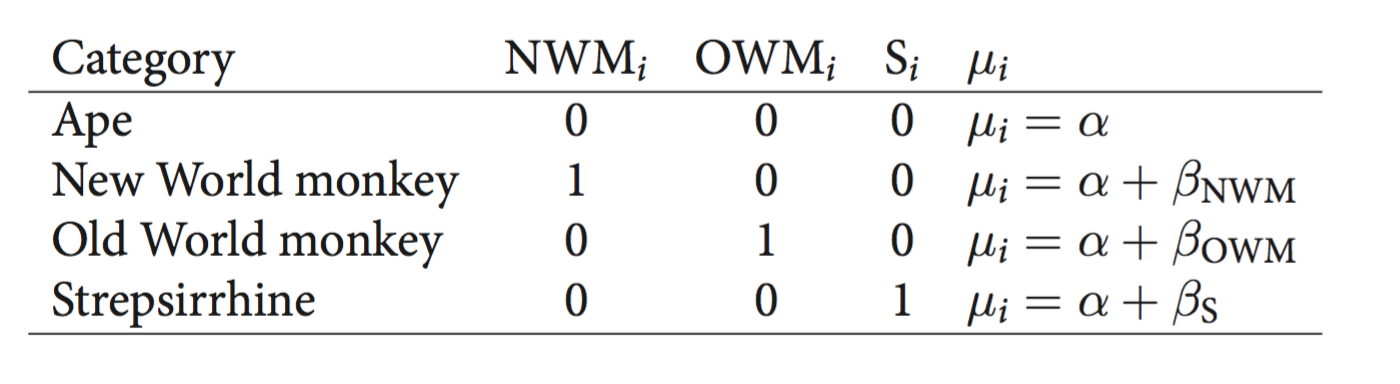
\includegraphics[width=0.66\linewidth]{figures/table} \end{center}

\ldots{}

\begin{Shaded}
\begin{Highlighting}[]
\NormalTok{priors \textless{}{-}}\StringTok{ }\KeywordTok{c}\NormalTok{(}
  \KeywordTok{prior}\NormalTok{(}\KeywordTok{normal}\NormalTok{(}\FloatTok{0.6}\NormalTok{, }\DecValTok{10}\NormalTok{), }\DataTypeTok{class =}\NormalTok{ Intercept),}
  \KeywordTok{prior}\NormalTok{(}\KeywordTok{normal}\NormalTok{(}\DecValTok{0}\NormalTok{, }\DecValTok{1}\NormalTok{), }\DataTypeTok{class =}\NormalTok{ b),}
  \KeywordTok{prior}\NormalTok{(}\KeywordTok{exponential}\NormalTok{(}\FloatTok{0.01}\NormalTok{), }\DataTypeTok{class =}\NormalTok{ sigma)}
\NormalTok{  )}

\NormalTok{mod10 \textless{}{-}}\StringTok{ }\KeywordTok{brm}\NormalTok{(}
\NormalTok{  kcal.per.g }\OperatorTok{\textasciitilde{}}\StringTok{ }\DecValTok{1} \OperatorTok{+}\StringTok{ }\NormalTok{clade.NWM }\OperatorTok{+}\StringTok{ }\NormalTok{clade.OWM }\OperatorTok{+}\StringTok{ }\NormalTok{clade.S,}
  \DataTypeTok{prior =}\NormalTok{ priors,}
  \DataTypeTok{family =}\NormalTok{ gaussian,}
  \DataTypeTok{data =}\NormalTok{ df5}
\NormalTok{  )}
\end{Highlighting}
\end{Shaded}

\begin{Shaded}
\begin{Highlighting}[]
\KeywordTok{summary}\NormalTok{(mod10)}
\end{Highlighting}
\end{Shaded}

\begin{verbatim}
##  Family: gaussian 
##   Links: mu = identity; sigma = identity 
## Formula: kcal.per.g ~ 1 + clade.NWM + clade.OWM + clade.S 
##    Data: df5 (Number of observations: 29) 
## Samples: 4 chains, each with iter = 2000; warmup = 1000; thin = 1;
##          total post-warmup samples = 4000
## 
## Population-Level Effects: 
##           Estimate Est.Error l-95% CI u-95% CI Rhat Bulk_ESS Tail_ESS
## Intercept     0.55      0.04     0.46     0.63 1.00     2982     2580
## clade.NWM     0.17      0.06     0.05     0.29 1.00     3279     2767
## clade.OWM     0.24      0.07     0.10     0.38 1.00     3791     3168
## clade.S      -0.04      0.07    -0.19     0.10 1.00     3443     2915
## 
## Family Specific Parameters: 
##       Estimate Est.Error l-95% CI u-95% CI Rhat Bulk_ESS Tail_ESS
## sigma     0.13      0.02     0.10     0.17 1.00     3237     2518
## 
## Samples were drawn using sampling(NUTS). For each parameter, Bulk_ESS
## and Tail_ESS are effective sample size measures, and Rhat is the potential
## scale reduction factor on split chains (at convergence, Rhat = 1).
\end{verbatim}

\ldots{}

\begin{Shaded}
\begin{Highlighting}[]
\CommentTok{\# retrieves posterior samples}
\NormalTok{post \textless{}{-}}\StringTok{ }\KeywordTok{posterior\_samples}\NormalTok{(mod10)}

\CommentTok{\# retrieves posterior samples for each category}
\NormalTok{mu.ape \textless{}{-}}\StringTok{ }\NormalTok{post}\OperatorTok{$}\NormalTok{b\_Intercept}
\NormalTok{mu.NWM \textless{}{-}}\StringTok{ }\NormalTok{post}\OperatorTok{$}\NormalTok{b\_Intercept }\OperatorTok{+}\StringTok{ }\NormalTok{post}\OperatorTok{$}\NormalTok{b\_clade.NWM}
\NormalTok{mu.OWM \textless{}{-}}\StringTok{ }\NormalTok{post}\OperatorTok{$}\NormalTok{b\_Intercept }\OperatorTok{+}\StringTok{ }\NormalTok{post}\OperatorTok{$}\NormalTok{b\_clade.OWM}
\NormalTok{mu.S \textless{}{-}}\StringTok{ }\NormalTok{post}\OperatorTok{$}\NormalTok{b\_Intercept }\OperatorTok{+}\StringTok{ }\NormalTok{post}\OperatorTok{$}\NormalTok{b\_clade.S}
\end{Highlighting}
\end{Shaded}

\begin{Shaded}
\begin{Highlighting}[]
\KeywordTok{precis}\NormalTok{(}\KeywordTok{data.frame}\NormalTok{(mu.ape, mu.NWM, mu.OWM, mu.S), }\DataTypeTok{prob =} \FloatTok{0.95}\NormalTok{)}
\end{Highlighting}
\end{Shaded}

\begin{verbatim}
##        Mean StdDev |0.95 0.95|
## mu.ape 0.55   0.04  0.46  0.63
## mu.NWM 0.71   0.04  0.63  0.80
## mu.OWM 0.79   0.05  0.68  0.89
## mu.S   0.51   0.06  0.39  0.62
\end{verbatim}

Si on s'intéresse à la différence entre deux groupes, on peut calculer la distribution postérieure de cette différence.

\begin{Shaded}
\begin{Highlighting}[]
\NormalTok{diff.NWM.OWM \textless{}{-}}\StringTok{ }\NormalTok{mu.NWM }\OperatorTok{{-}}\StringTok{ }\NormalTok{mu.OWM}
\KeywordTok{quantile}\NormalTok{(diff.NWM.OWM, }\DataTypeTok{probs =} \KeywordTok{c}\NormalTok{(}\FloatTok{0.025}\NormalTok{, }\FloatTok{0.5}\NormalTok{, }\FloatTok{0.975}\NormalTok{) )}
\end{Highlighting}
\end{Shaded}

\begin{verbatim}
##        2.5%         50%       97.5% 
## -0.21369114 -0.07307724  0.06310590
\end{verbatim}

\begin{Shaded}
\begin{Highlighting}[]
\KeywordTok{plotPost}\NormalTok{(diff.NWM.OWM, }\DataTypeTok{compVal =} \DecValTok{0}\NormalTok{, }\DataTypeTok{ROPE =} \KeywordTok{c}\NormalTok{(}\OperatorTok{{-}}\FloatTok{0.1}\NormalTok{, }\FloatTok{0.1}\NormalTok{) )}
\end{Highlighting}
\end{Shaded}

\begin{center}
\includegraphics[width=0.75\linewidth]{IMSB_files/figure-latex/plotpost-mod10-ch4-1} \end{center}

Une autre manière de considérer les variables catégorielles consiste à construire un vecteur d'intercepts, avec un intercept par catégorie.

\[
\begin{aligned}
\color{orangered}{k_{i}} \ &\color{orangered}{\sim \mathrm{Normal}(\mu_{i}, \sigma)} \\
\color{black}{\mu_{i}} \ &\color{black}{= \alpha_{\text{clade}[i]}} \\
\color{steelblue}{\alpha_{\text{clade}[i]}} \ &\color{steelblue}{\sim \mathrm{Normal}(0.6, 10)} \\
\color{steelblue}{\sigma} \ &\color{steelblue}{\sim \mathrm{Exponential}(0.01)}
\end{aligned}
\]

Comme on a vu avec l'exemple du genre, \texttt{brms} ``comprend'' automatiquement que c'est ce qu'on veut faire lorsqu'on fit un modèle sans intercept et avec un prédicteur catégoriel (codé en facteur).

\begin{Shaded}
\begin{Highlighting}[]
\NormalTok{priors \textless{}{-}}\StringTok{ }\KeywordTok{c}\NormalTok{(}
  \KeywordTok{prior}\NormalTok{(}\KeywordTok{normal}\NormalTok{(}\FloatTok{0.6}\NormalTok{, }\DecValTok{10}\NormalTok{), }\DataTypeTok{class =}\NormalTok{ b),}
  \KeywordTok{prior}\NormalTok{(}\KeywordTok{exponential}\NormalTok{(}\FloatTok{0.01}\NormalTok{), }\DataTypeTok{class =}\NormalTok{ sigma)}
\NormalTok{  )}

\NormalTok{mod11 \textless{}{-}}\StringTok{ }\KeywordTok{brm}\NormalTok{(}
  \CommentTok{\# modèle sans intercept avec seulement un prédicteur catégoriel (facteur)}
\NormalTok{  kcal.per.g }\OperatorTok{\textasciitilde{}}\StringTok{ }\DecValTok{0} \OperatorTok{+}\StringTok{ }\NormalTok{clade,}
  \DataTypeTok{prior =}\NormalTok{ priors,}
  \DataTypeTok{family =}\NormalTok{ gaussian,}
  \DataTypeTok{data =}\NormalTok{ df5}
\NormalTok{  )}
\end{Highlighting}
\end{Shaded}

\begin{Shaded}
\begin{Highlighting}[]
\KeywordTok{summary}\NormalTok{(mod11)}
\end{Highlighting}
\end{Shaded}

\begin{verbatim}
##  Family: gaussian 
##   Links: mu = identity; sigma = identity 
## Formula: kcal.per.g ~ 0 + clade 
##    Data: df5 (Number of observations: 29) 
## Samples: 4 chains, each with iter = 2000; warmup = 1000; thin = 1;
##          total post-warmup samples = 4000
## 
## Population-Level Effects: 
##                     Estimate Est.Error l-95% CI u-95% CI Rhat Bulk_ESS Tail_ESS
## cladeApe                0.55      0.04     0.46     0.63 1.00     4075     3066
## cladeNewWorldMonkey     0.71      0.04     0.63     0.80 1.00     5058     2527
## cladeOldWorldMonkey     0.79      0.05     0.69     0.89 1.00     5014     3140
## cladeStrepsirrhine      0.51      0.06     0.39     0.63 1.00     4081     2622
## 
## Family Specific Parameters: 
##       Estimate Est.Error l-95% CI u-95% CI Rhat Bulk_ESS Tail_ESS
## sigma     0.13      0.02     0.10     0.18 1.00     3441     2891
## 
## Samples were drawn using sampling(NUTS). For each parameter, Bulk_ESS
## and Tail_ESS are effective sample size measures, and Rhat is the potential
## scale reduction factor on split chains (at convergence, Rhat = 1).
\end{verbatim}

\hypertarget{interaction}{%
\subsection{Interaction}\label{interaction}}

Jusque là, les prédicteurs du modèle entretenaientt des relations mutuellement indépendantes. Et si nous souhaitions que ces relations soient \textbf{conditionnelles}, ou \textbf{dépendantes} les unes des autres ?

Par exempl e: on s'intéresse à la pousse des tulipes selon la quantité de lumière reçue et l'humidité du sol. Il se pourrait que la relation entre quantité de lumière reçue et pousse des tulipes soit différente selon l'humidité du sol. En d'autres termes, il se pourrait que la relation entre quantité de lumière reçue et pousse des tulipe soit \textbf{conditionnelle} à l'humidité du sol\ldots{}

\begin{Shaded}
\begin{Highlighting}[]
\KeywordTok{data}\NormalTok{(tulips)}
\NormalTok{df6 \textless{}{-}}\StringTok{ }\NormalTok{tulips}

\KeywordTok{head}\NormalTok{(df6, }\DecValTok{10}\NormalTok{)}
\end{Highlighting}
\end{Shaded}

\begin{verbatim}
##    bed water shade blooms
## 1    a     1     1   0.00
## 2    a     1     2   0.00
## 3    a     1     3 111.04
## 4    a     2     1 183.47
## 5    a     2     2  59.16
## 6    a     2     3  76.75
## 7    a     3     1 224.97
## 8    a     3     2  83.77
## 9    a     3     3 134.95
## 10   b     1     1  80.10
\end{verbatim}

Modèle sans interaction :

\[
\begin{aligned}
B_{i} &\sim \mathrm{Normal}(\mu, \sigma) \\
\mu_{i} &= \alpha + \beta_{W} W_{i} + \beta_{S} S_{i} \\
\end{aligned}
\]

Modèle avec interaction :

\[
\begin{aligned}
B_{i} &\sim \mathrm{Normal}(\mu, \sigma) \\
\mu_{i} &= \alpha + \beta_{W} W_{i} + \beta_{S} S_{i} + \beta_{WS} W_{i} S_{i}\\
\end{aligned}
\]

On centre les prédicteurs (pour faciliter l'interprétation des paramètres).

\begin{Shaded}
\begin{Highlighting}[]
\NormalTok{df6}\OperatorTok{$}\NormalTok{shade.c \textless{}{-}}\StringTok{ }\NormalTok{df6}\OperatorTok{$}\NormalTok{shade }\OperatorTok{{-}}\StringTok{ }\KeywordTok{mean}\NormalTok{(df6}\OperatorTok{$}\NormalTok{shade)}
\NormalTok{df6}\OperatorTok{$}\NormalTok{water.c \textless{}{-}}\StringTok{ }\NormalTok{df6}\OperatorTok{$}\NormalTok{water }\OperatorTok{{-}}\StringTok{ }\KeywordTok{mean}\NormalTok{(df6}\OperatorTok{$}\NormalTok{water)}
\end{Highlighting}
\end{Shaded}

\begin{Shaded}
\begin{Highlighting}[]
\NormalTok{priors \textless{}{-}}\StringTok{ }\KeywordTok{c}\NormalTok{(}
  \KeywordTok{prior}\NormalTok{(}\KeywordTok{normal}\NormalTok{(}\DecValTok{130}\NormalTok{, }\DecValTok{100}\NormalTok{), }\DataTypeTok{class =}\NormalTok{ Intercept),}
  \KeywordTok{prior}\NormalTok{(}\KeywordTok{normal}\NormalTok{(}\DecValTok{0}\NormalTok{, }\DecValTok{100}\NormalTok{), }\DataTypeTok{class =}\NormalTok{ b),}
  \KeywordTok{prior}\NormalTok{(}\KeywordTok{exponential}\NormalTok{(}\FloatTok{0.01}\NormalTok{), }\DataTypeTok{class =}\NormalTok{ sigma)}
\NormalTok{  )}

\NormalTok{mod12 \textless{}{-}}\StringTok{ }\KeywordTok{brm}\NormalTok{(}
\NormalTok{  blooms }\OperatorTok{\textasciitilde{}}\StringTok{ }\DecValTok{1} \OperatorTok{+}\StringTok{ }\NormalTok{water.c }\OperatorTok{+}\StringTok{ }\NormalTok{shade.c,}
  \DataTypeTok{prior =}\NormalTok{ priors,}
  \DataTypeTok{family =}\NormalTok{ gaussian,}
  \DataTypeTok{data =}\NormalTok{ df6}
\NormalTok{  )}
\end{Highlighting}
\end{Shaded}

\begin{Shaded}
\begin{Highlighting}[]
\NormalTok{mod13 \textless{}{-}}\StringTok{ }\KeywordTok{brm}\NormalTok{(}
\NormalTok{  blooms }\OperatorTok{\textasciitilde{}}\StringTok{ }\DecValTok{1} \OperatorTok{+}\StringTok{ }\NormalTok{water.c }\OperatorTok{*}\StringTok{ }\NormalTok{shade.c,}
  \CommentTok{\# equivalent to blooms \textasciitilde{} 1 + water.c + shade.c + water.c:shade.c}
  \DataTypeTok{prior =}\NormalTok{ priors,}
  \DataTypeTok{family =}\NormalTok{ gaussian,}
  \DataTypeTok{data =}\NormalTok{ df6}
\NormalTok{  )}
\end{Highlighting}
\end{Shaded}

\ldots{}

\begin{verbatim}
##                term     mod12     mod13
## 1       b_Intercept 128.99761 128.78220
## 2         b_water.c  73.89508  74.53079
## 3         b_shade.c -40.95156 -40.95594
## 4             sigma  63.50477  51.17996
## 5 b_water.c:shade.c        NA -51.64005
\end{verbatim}

\begin{itemize}
\item
  L'intercept \(\alpha\) représente la valeur attendue de \texttt{blooms} quand \texttt{water} et \texttt{shade} sont à 0 (i.e., la moyenne générale de la variable dépendante).
\item
  La pente \(\beta_{W}\) nous donne la valeur attendue de changement de \texttt{blooms} quand \texttt{water} augmente d'une unité et \texttt{shade} est à sa valeur moyenne. On voit qu'augmenter la quantité d'eau est très bénéfique.
\item
  La pente \(\beta_{S}\) nous donne la valeur attendue de changement de \texttt{blooms} quand \texttt{shade} augmente d'une unité et \texttt{water} est à sa valeur moyenne. On voit qu'augmenter la ``quantité d'ombre'' (diminuer l'exposition à la lumière) est plutôt délétère.
\item
  La pente \(\beta_{WS}\) nous renseigne sur l'effet attendu de \texttt{water} sur \texttt{blooms} quand \texttt{shade} augment d'une unité (et réciproquement).
\end{itemize}

Dans un modèle qui inclut un effet d'interaction, l'effet d'un prédicteur sur la mesure va dépendre de la valeur de l'autre prédicteur. La meilleure manière de représenter cette dépendance est de plotter la relation entre un prédicteur et la mesure, à différentes valeurs de l'autre prédicteur.

\begin{center}
\includegraphics[width=0.75\linewidth]{IMSB_files/figure-latex/plot-models-ch4-1} \end{center}

L'effet d'interaction nous indique que les tulipes ont besoin à la fois d'eau et de lumière pour pousser, mais aussi qu'à de faibles niveaux d'humidité, la luminosité a peu d'effet, tandis que cet effet est plus important à haut niveau d'humidité.

Cette explication vaut de manière \textbf{symétrique} pour l'effet de l'humidité sur la relation entre la luminosité et la pousse des plantes.

\hypertarget{appendix-annexes}{%
\appendix}


\hypertarget{glossaire}{%
\chapter{Glossaire}\label{glossaire}}

\textbf{Facteur de Bayes (\emph{Bayes factor})} : Support relatif fourni par un jeu de données pour deux hypothèses alternatives. Si on considère deux hypothèses \(\mathcal{H}_{1}\) et \(\mathcal{H}_{2}\) et des données \(x\), alors le facteur de Bayes est \(p(x \ | \ \mathcal{H}_{1}) / p(x \ | \ \mathcal{H}_{2})\). Ce dernier peut-être inteprêté comme un ``facteur de mise à jour'' du rapport des chances a priori (i.e., avant de prendre connaissance des données) vers le rapport des chances a posteriori (i.e., après avoir pris connaissance des données).

\textbf{Vraisemblance (\emph{Likelihood})} : Une mesure du support fourni par les données pour certaines valeurs de paramètres. Après avoir observé des donnés \(x\), la vraisemblance d'un paramètre \(\theta\) est proportionnelle à \(p(x \ | \ \theta)\).

\hypertarget{bibliographie}{%
\chapter*{Bibliographie}\label{bibliographie}}
\addcontentsline{toc}{chapter}{Bibliographie}

\markboth{Bibliographie}{Bibliographie}

\setlength{\parindent}{-0.5in}
\setlength{\parskip}{8pt}

\hypertarget{refs}{}
\begin{cslreferences}
\leavevmode\hypertarget{ref-R-rmarkdown}{}%
Allaire, J., Xie, Y., McPherson, J., Luraschi, J., Ushey, K., Atkins, A., \ldots{} Iannone, R. (2020). \emph{Rmarkdown: Dynamic documents for r}. Retrieved from \url{https://CRAN.R-project.org/package=rmarkdown}

\leavevmode\hypertarget{ref-R-papaja}{}%
Aust, F., \& Barth, M. (2020). \emph{Papaja: Prepare reproducible apa journal articles with r markdown}. Retrieved from \url{https://github.com/crsh/papaja}

\leavevmode\hypertarget{ref-R-brms}{}%
Bürkner, P.-C. (2020). \emph{Brms: Bayesian regression models using 'stan'}. Retrieved from \url{https://CRAN.R-project.org/package=brms}

\leavevmode\hypertarget{ref-carnap_logical_1950}{}%
Carnap, R. (1950). \emph{Logical Foundations of Probability}. Chicago{]}University of Chicago Press.

\leavevmode\hypertarget{ref-hanck_introduction_2018}{}%
Hanck, C., Arnold, M., Gerber, A., \& Schmelzer, M. (2018). \emph{Introduction to Econometrics with R}. Retrieved from \url{https://www.econometrics-with-r.org/}

\leavevmode\hypertarget{ref-sep-probability-interpret}{}%
Hájek, A. (2019). Interpretations of probability. In E. N. Zalta (Ed.), \emph{The stanford encyclopedia of philosophy} (Fall 2019). Metaphysics Research Lab, Stanford University. Retrieved from \url{https://plato.stanford.edu/archives/fall2019/entries/probability-interpret/}

\leavevmode\hypertarget{ref-jaynes_bayesian_1986}{}%
Jaynes, E. T. (1986). Bayesian Methods: General Background. In \emph{Maximum Entropy and Bayesian Methods in Applied Statistics: Proceedings of the Fourth Maximum Entropy Workshop University of Calgary, 1984}. \url{https://doi.org/10.1017/CBO9780511569678.003}

\leavevmode\hypertarget{ref-keynes_treatise_1921}{}%
Keynes, J. M. (1921). \emph{A Treatise On Probability}. Macmillan And Co., Retrieved from \url{http://archive.org/details/treatiseonprobab007528mbp}

\leavevmode\hypertarget{ref-kolmogorov_foundations_1933}{}%
Kolmogorov, A. N. (1933). \emph{Foundations of the theory of probability}. New York, USA: Chelsea Publishing Company.

\leavevmode\hypertarget{ref-lindley_philosophy_2001}{}%
Lindley, D. V. (2001). The Philosophy of Statistics. \emph{Journal of the Royal Statistical Society: Series D (the Statistician)}, \emph{49}(3), 293--337. \url{https://doi.org/10.1111/1467-9884.00238}

\leavevmode\hypertarget{ref-mcelreath_statistical_2016}{}%
McElreath, R. (2016). \emph{Statistical rethinking: A Bayesian course with examples in R and Stan}. Boca Raton: CRC Press/Taylor \& Francis Group.

\leavevmode\hypertarget{ref-mcelreath_statistical_2020}{}%
McElreath, R. (2020). \emph{Statistical rethinking: A Bayesian course with examples in R and Stan} (2nd ed.). Boca Raton: Taylor; Francis, CRC Press.

\leavevmode\hypertarget{ref-R-base}{}%
R Core Team. (2019). \emph{R: A language and environment for statistical computing}. Vienna, Austria: R Foundation for Statistical Computing. Retrieved from \url{https://www.R-project.org/}

\leavevmode\hypertarget{ref-talbot_critical_2015}{}%
Talbot, M. (2015). \emph{Critical Reasoning: A Romp through the Foothills of Logic for the Complete Beginner}. (C. Wood, Ed.) (1 edition). CreateSpace Independent Publishing Platform.

\leavevmode\hypertarget{ref-R-tidyverse}{}%
Wickham, H. (2019). \emph{Tidyverse: Easily install and load the 'tidyverse'}. Retrieved from \url{https://CRAN.R-project.org/package=tidyverse}

\leavevmode\hypertarget{ref-R-ggplot2}{}%
Wickham, H., Chang, W., Henry, L., Pedersen, T. L., Takahashi, K., Wilke, C., \ldots{} Yutani, H. (2019). \emph{Ggplot2: Create elegant data visualisations using the grammar of graphics}. Retrieved from \url{https://CRAN.R-project.org/package=ggplot2}

\leavevmode\hypertarget{ref-R-bookdown}{}%
Xie, Y. (2020a). \emph{Bookdown: Authoring books and technical documents with r markdown}. Retrieved from \url{https://CRAN.R-project.org/package=bookdown}

\leavevmode\hypertarget{ref-R-knitr}{}%
Xie, Y. (2020b). \emph{Knitr: A general-purpose package for dynamic report generation in r}. Retrieved from \url{https://CRAN.R-project.org/package=knitr}
\end{cslreferences}

\end{document}
